\documentclass[12pt]{memoir}

\def\nsemestre {II}
\def\nterm {Fall}
\def\nyear {2023}
\def\nprofesor {Renzo Cavalieri}
\def\nsigla {MATH676}
\def\nsiglahead {Tropical Geometry}
\def\nlang {ENG}
%\def\darktheme{}
\let\footruleskip\relax %%FADIR

\makeatletter
\ifx \nauthor\undefined
  \def\nauthor{Ignacio Rojas}
\else
\fi

\ifx \nextra \undefined
\ifx \nlang \undefined
\author{Basado en las clases impartidas por \nprofesor \\\small Notas tomadas por \nauthor}
\else
\author{Based on the lectures by \nprofesor \\\small Notes written by \nauthor}
\fi
\else
\author{\nauthor}
\fi
\date{\nterm\ \nyear}

%%%%%%%%%%%%%
%% 1. Pacotes
%%%%%%%%%%%%%

\usepackage{alltt}
\usepackage{amsfonts}
\usepackage{amsmath}
\usepackage{amssymb}
\usepackage{amsthm}
\usepackage{algorithm}
\usepackage[noend]{algpseudocode}
\usepackage{array}
\newcommand\hmmax{0} % default 3
\newcommand\bmmax{0} % default 4 %%tex.se/3676,219310
%\usepackage{bbold}
\usepackage{bm}
\usepackage{booktabs}
%\usepackage{caption}
%\usepackage{cancel}
%\usepackage{dsfont}
\usepackage{esint}
\usepackage{fancyhdr}
\usepackage{graphicx}
\usepackage[utf8]{inputenc}
\usepackage{listings}
\usepackage{mathabx}
\usepackage[cal=euler]{mathalfa}
%\usepackage[cal=euler,frak=euler]{mathalfa} % mathcal (JIRR) precisabamos correr initexmf --mkmaps en cmd JCVDG
\usepackage{mathdots}
\usepackage{mathrsfs}
%\usepackage{mathtools}
\usepackage{microtype}
\usepackage{multicol}
\usepackage{multirow}
\usepackage[theoremfont,largesc,tighter,osf]{newpxtext} %JCV Diff
\let\widering\undefined
%\usepackage[bigdelims,vvarbb]{newpxmath} %JCVDG
%por alguna razón esto afectaba las tildes en \min, \lim y demás
%\usepackage{pdflscape}
\usepackage{pgfplots}
\usepackage{physics}
\usepackage{siunitx}
\usepackage{slashed}
%\usepackage{stmaryrd}
%\SetSymbolFont{stmry}{bold}{U}{stmry}{m}{n}
%\usepackage{subfigure}
\usepackage{subcaption}
\usepackage{tabularx}
\usepackage[breakable,skins]{tcolorbox}
\usepackage{textcomp} %%JCVDG
\usepackage{tikz}
\usepackage{tkz-euclide}
\usepackage[normalem]{ulem}
\usepackage[all]{xy}
\usepackage{imakeidx}
\ifx \nlang \undefined
\usepackage[spanish]{babel}
\else\fi 
\usepackage{wrapfig}

%%%%%%%%%%%%%%%%%%%%
%% 2. Document Setup
%%%%%%%%%%%%%%%%%%%%

\ifx \nextra \undefined
    \ifx \nlang \undefined
    \makeindex[intoc, title=Índice Analítico] %Título de índice analítico
    %El índice general es aquel en el que se indican los capítulos, títulos y subtítulos del libro.
    %Índice onomástico es donde aparece el nombre de personas mencionadas en el texto, por orden alfabético con el número de las páginas donde aparecen.
    %El índice analítico se refiere a los temas y conceptos que aparecen en el libro
    \indexsetup{othercode={\fancyhead[LE]{\emph{Índice Analítico}}}}
    \else
    \makeindex[intoc, title=Index] 
    \indexsetup{othercode={\fancyhead[LE]{\emph{Index}}}}
    \fi
  \usepackage[pdftex,
    hidelinks,
    pdfauthor={\nauthor},
    pdfsubject={Notas: \nsiglahead\ \nsemestre-\nyear},
    pdftitle={Semestre \nsemestre\ - \nsigla},
  pdfkeywords={UCR Costa Rica Matem\'aticas Mate \nsemestre\ \nterm\ \nyear\ \nsiglahead}]{hyperref}
  \title{\nsigla\ --- \nsiglahead}
\else
  \usepackage[pdftex,
     hidelinks,
    pdfauthor={\nauthor},
    pdfsubject={\nextra \nsiglahead\ \nsemestre-\nyear},
    pdftitle={Semestre \nsemestre\ - \nsigla},
  pdfkeywords={UCR Costa Rica Matem\'aticas Mate \nsemestre\ \nterm\ \nyear\ \nsiglahead\ \nextra}]{hyperref}

  \title{\nsigla\ --- \nsiglahead \\ {\Large \nextra}}
  \renewcommand\printindex{}
\fi

\pgfplotsset{compat=1.12}


\pagestyle{fancy}
\setlength{\headheight}{15.72pt} %preceding warning said make it at least this


\ifx \nsiglahead \undefined
\def\nsiglahead{\nsigla}
\fi

\lhead{} %%%empty lhead
\rfoot{\thepage}

\ifx \nextra \undefined
  \chead{
    \ifnum\thepage=1
    \else
      \ifx \nlang \undefined
      \textbf{Notas \nsiglahead\ \nsemestre-\nyear}
      \else
      \textbf{Notes \nsiglahead\ \nsemestre-\nyear}
      \fi
    \fi}
  \rhead{}%\firstxmark} % Top right header
\else
%    \chead{
%    \ifnum\thepage=1
%    \else
%      \textbf{Notas \nsiglahead\ \nsemestre-\nyear \ (\nextra)}
%    \fi}
     \chead{
       \textbf{\nextra\ \nsigla\ \nsemestre-\nyear}
     }
     \rhead{
       \textbf{\nauthor}
     }
\fi
\lfoot{}%\lastxmark} % Bottom left footer
\cfoot{} % Bottom center footer

\usetikzlibrary{arrows.meta}
\usetikzlibrary{decorations.markings}
\usetikzlibrary{decorations.pathmorphing}
\usetikzlibrary{positioning}
\usetikzlibrary{fadings}
\usetikzlibrary{intersections}
\usetikzlibrary{cd}

\ifx \nhtml \undefined
\else
  \renewcommand\printindex{}
  \DisableLigatures[f]{family = *}
  \let\Contentsline\contentsline
  \renewcommand\contentsline[3]{\Contentsline{#1}{#2}{}}
  \renewcommand{\@dotsep}{10000}
  \newlength\currentparindent
  \setlength\currentparindent\parindent

  \newcommand\@minipagerestore{\setlength{\parindent}{\currentparindent}}
  \usepackage[active,tightpage,pdftex]{preview}
  \renewcommand{\PreviewBorder}{0.1cm}

  \newenvironment{stretchpage}%
  {\begin{preview}\begin{minipage}{\hsize}}%
    {\end{minipage}\end{preview}}
  \AtBeginDocument{\begin{stretchpage}}
  \AtEndDocument{\end{stretchpage}}

  \newcommand{\@@newpage}{\end{stretchpage}\begin{stretchpage}}

  \let\@real@section\section
  \renewcommand{\section}{\@@newpage\@real@section}
  \let\@real@subsection\subsection
  \renewcommand{\subsection}{\@ifstar{\@real@subsection*}{\@@newpage\@real@subsection}}
\fi
\ifx \ntrim \undefined
\usepackage[shortlabels]{enumitem} %mfw package order matters por savetrees
\else
  \usepackage{geometry}
  \geometry{
    papersize={379pt, 699pt},
    textwidth=345pt,
    textheight=596pt,
    left=17pt,
    top=54pt,
    right=17pt
  }
  \headwidth=345pt
 \usepackage[extreme]{savetrees}
\fi

\ifx \darktheme\undefined
\else
\pagecolor[rgb]{0.2,0.231,0.302}%{0.23,0.258,0.321}
\color[rgb]{1,1,1}
\fi

\ifx \nextra \undefined
\let\@real@maketitle\maketitle
\renewcommand{\maketitle}{\@real@maketitle\begin{center}\begin{minipage}[c]{0.9\textwidth}\centering\footnotesize 
  \ifx \nlang \undefined
  Estas notas no están respaldadas por los profesores y han sido modificadas (a menudo de manera significativa) después de las clases. No están lejos de ser representaciones precisas de lo que realmente se dio en clase y en particular todos los errores son casi seguramente míos.
  \else 
  Please note that these notes were not provided or endorsed by the lecturer and have been significantly altered after the class. They may not accurately reflect the content covered in class and any errors are solely my responsibility.
  \fi
\end{minipage}\end{center}}
\else
\fi

\def\moverlay{\mathpalette\mov@rlay}
\def\mov@rlay#1#2{\leavevmode\vtop{%
   \baselineskip\z@skip \lineskiplimit-\maxdimen
   \ialign{\hfil$\m@th#1##$\hfil\cr#2\crcr}}}
\newcommand{\charfusion}[3][\mathord]{
    #1{\ifx#1\mathop\vphantom{#2}\fi
        \mathpalette\mov@rlay{#2\cr#3}
      }
    \ifx#1\mathop\expandafter\displaylimits\fi}

%%%%%%%%%%%%%%%%%%%%%%%%%%%%%%
%% 2.1 Some internal machinery
%%%%%%%%%%%%%%%%%%%%%%%%%%%%%%

\makeatletter
\renewcommand{\section}{\@startsection{section}{1}{\z@}%
							 {-3.25ex \@plus -1ex \@minus -.2ex}%
							 {1.5ex \@plus.2ex}%
							 {\normalfont\large\bfseries}}
\renewcommand{\subsection}{\@startsection{subsection}{2}{\z@}%
							 {-3.25ex \@plus -1ex \@minus -.2ex}%
							 {1.5ex \@plus .2ex}%
               {\normalfont\normalsize\bfseries}}
\newcommand*{\defeq}{\!\mathrel{\rlap{%
             \raisebox{0.3ex}{$\m@th\cdot$}}%
             \raisebox{-0.3ex}{$\m@th\cdot$}}%
                    =\!}
\makeatother
\ifx\ntrim\undefined
\newcommand{\coursetitle}{\nsigla: \nsiglahead}
\ifx\nextra\undefined
\pagestyle{ruled}
\makeoddhead{ruled}{\coursetitle}{}{\rightmark}
\else\fi
\settypeblocksize{49pc}{37pc}{*}
\setlrmargins{*}{*}{1.2}
\setulmargins{*}{*}{0.8}
\setheadfoot{16pt}{30pt}
\setheaderspaces{*}{1.5pc}{1}
\setmarginnotes{1pt}{1pt}{1pt}
\checkandfixthelayout

\setlength{\unitlength}{3pt}
\setlength{\hfuzz}{1pt}

\setlength{\fboxsep}{6pt}

\setlength{\footskip}{17pt}

\linespread{1.1}
\else\fi
\renewcommand{\cftdotsep}{\cftnodots} %%% no dots in ToC
\setpnumwidth{2em}  %%% width of page-number box in ToC


\newcommand{\stophere}{\relax} %% can be changed to `\endinput'
% \newcommand{\stophere}{\endinput} %% can be changed to `\relax'


\DeclareRobustCommand{\qned}{\ifmmode
  \else \leavevmode\unskip\penalty9999 \hbox{}\nobreak\hfill \fi
  \quad\hbox{\qnedsymbol}}
\newcommand{\qnedsymbol}{$\boxminus$} %% No-proofs end with `\qned'

\DeclareRobustCommand{\qef}{\ifmmode
  \else \leavevmode\unskip\penalty9999 \hbox{}\nobreak\hfill \fi
  \quad\hbox{\qefsymbol}}
\newcommand{\qefsymbol}{$\lozenge$} %% Examples end with `\qef'
\def\enddefn{\qef\endtrivlist}      %% `\qef' automático en defns
\def\endejem{\qef\endtrivlist}      %% `\qef' automático en ejemplos

\newcommand{\hideqed}{\renewcommand{\qed}{}} %% to suppress `\qed'
\newcommand{\hideqef}{\renewcommand{\qef}{}} %% to suppress `\qef'

% \newcommand{\ldbrack}{\ensuremath{[\mskip-2.5mu[}} %% corchetes [[
% \newcommand{\rdbrack}{\ensuremath{]\mskip-2.5mu]}} %% corchetes ]]

\newcommand{\stroke}{\mathbin|}     %% (for `\bbraket' and such)

\newcommand{\rtri}{\blacktriangleright} %% (for `\marker' and such)
\newcommand{\tribar}{|\mkern-2mu|\mkern-2mu|} %% norma triple: |||


%% Formatting changes:

\renewcommand{\labelitemi}{$\diamond$} %% instead of bullets

\renewcommand{\theenumi}{\alph{enumi}}  %% use lowercase letters
\renewcommand{\labelenumi}{\textup{(\theenumi)}} %% inside parentheses

%%%%%%%%%%%%%%
%% 2.2. Colors
%%%%%%%%%%%%%%

\definecolor{MATLABgreen}{RGB}{28,172,0} % color values Red, Green, Blue
\definecolor{MATLABlila}{RGB}{170,55,241}
\definecolor{dankBlue}{RGB}{51,60,77} % color values Red, Green, Blue
\definecolor{dankBlueLite}{RGB}{82,97,125} % color values Red, Green, Blue
\definecolor{celesUCR}{RGB}{0,192,243}
\definecolor{azulUCR}{RGB}{0,93,164}
\definecolor{verdeUCR}{RGB}{109,192,103}
\definecolor{yelloUCR}{RGB}{255,224,106}

%%%%%%%%%%%%%%%%%%%%%%%%%%%
%% 3. Theorems and suchlike
%%%%%%%%%%%%%%%%%%%%%%%%%%%

\ifx\nlang\undefined

\theoremstyle{plain}
\ifx \nextra \undefined
\newtheorem{Th}{Teorema}[section]      %%% Theorem 1.1.1
\newtheorem{Tmon}[Th]{Teoremón}
\newtheorem{Prop}[Th]{Proposición}     %%% Proposition 1.1.2
\newtheorem{Lem}[Th]{Lema}             %%% Lemma 1.1.3
\newtheorem{Cor}[Th]{Corolario}        %%% Corollary 1.1.4
\else
\newtheorem{Th}{Teorema}               %%% Theorem 1.1.1
\newtheorem{Tmon}{Teoremón}
\newtheorem{Prop}{Proposición}         %%% Proposition 1.1.2
\newtheorem{Lem}{Lema}                 %%% Lemma 3
\newtheorem{Cor}{Corolario}            %%% Corollary 4
\fi
\newtheorem*{nonum-Th}{Teorema}        %%% No-numbered Theorem
\newtheorem*{nonum-Cor}{Corolario}     %%% No-numbered Corollary

\theoremstyle{definition}
\ifx \nextra \undefined
\newtheorem{Def}[Th]{Definición}       %%% Definition 1.1.5
\newtheorem{Ex}[Th]{Ejemplo}           %%% Example 1.1.6
\newtheorem{Ej}[Th]{Ejercicio}         %%% Ejercicio 1.1.7
\else
\newtheorem{Def}{Definición}           %%% Definition 5
\newtheorem{Ex}{Ejemplo}               %%% Example 6
\newtheorem{Ej}{Ejercicio}             %%% Ejercicio 7
\fi
\newtheorem{Hec}[Th]{Hecho}            %%% Hecho 1.1.8
\newtheorem*{nonum-Def}{Definición}    %%% No number Definition
\newtheorem*{nonum-Ex}{Ejemplo}        %%% No number Example
\newtheorem*{nonum-Ej}{Ejercicio}      %%% No number Ejercicio
\newtheorem*{nonum-Hec}{Hecho}         %%% No number Fact


\theoremstyle{remark}
\newtheorem{Rmk}[Th]{Observación}      %%%Remark 1.1.9
\newtheorem*{nonum-Rmk}{Observación}         %%% No number Fact
\newtheorem*{Notn}{Notaci\'on}        %% Notaciones
\newtheorem*{Warn}{Advertencia}       %% Advertencias
\newtheorem*{Qn}{Pregunta}            %% Pregunta

\else

\theoremstyle{plain}
\ifx \nextra \undefined
\newtheorem{Th}{Theorem}[section]      %%% Theorem 1.1.1
\newtheorem{Tmon}[Th]{Teoremón}
\newtheorem{Prop}[Th]{Proposition}     %%% Proposition 1.1.2
\newtheorem{Lem}[Th]{Lemma}             %%% Lemma 1.1.3
\newtheorem{Cor}[Th]{Corollary}        %%% Corollary 1.1.4
\else
\newtheorem{Th}{Theorem}               %%% Theorem 1.1.1
\newtheorem{Tmon}{Teoremón}
\newtheorem{Prop}{Proposition}         %%% Proposition 1.1.2
\newtheorem{Lem}{Lemma}                 %%% Lemma 3
\newtheorem{Cor}{Corollary}            %%% Corollary 4
\fi
\newtheorem*{nonum-Th}{Theorem}        %%% No-numbered Theorem
\newtheorem*{nonum-Cor}{Corollary}     %%% No-numbered Corollary

\theoremstyle{definition}
\ifx \nextra \undefined
\newtheorem{Def}[Th]{Definition}       %%% Definition 1.1.5
\newtheorem{Ex}[Th]{Example}           %%% Example 1.1.6
\newtheorem{Ej}[Th]{Exercise}         %%% Exercise 1.1.7
\else
\newtheorem{Def}{Definition}           %%% Definition 5
\newtheorem{Ex}{Example}               %%% Example 6
\newtheorem{Ej}{Exercise}             %%% Exercise 7
\fi
\newtheorem{Hec}[Th]{Fact}            %%% Fact 1.1.8
\newtheorem*{nonum-Def}{Definition}    %%% No number Definition
\newtheorem*{nonum-Ex}{Example}        %%% No number Example
\newtheorem*{nonum-Ej}{Exercise}      %%% No number Exercise
\newtheorem*{nonum-Hec}{Fact}         %%% No number Fact


\theoremstyle{remark}
\newtheorem{Rmk}[Th]{Remark}      %%%Remark 1.1.9
\newtheorem*{nonum-Rmk}{Remark}         %%% No number Fact
\newtheorem*{Notn}{Notation}        %% Notaciones
\newtheorem*{Warn}{Warning}       %% Warnings
\newtheorem*{Qn}{Question}            %% Question

\fi 

\numberwithin{equation}{section}

\setlength{\parindent}{3ex}

% \renewcommand{\labelitemi}{--}
% \renewcommand{\labelitemii}{$\circ$}
% \renewcommand{\labelenumi}{(\roman{*})}

%\let\stdsection\section
%\renewcommand\section{\newpage\stdsection}

\newcommand\qedsym{\hfill\ensuremath{\square}}
% Strike through
\def\st{\bgroup \ULdepth=-.55ex \ULset}

%%%%%%%%% === My T Color Box === %%%%%%%%%%%%%%

\ifx\nlang\undefined
\ifx \darktheme\undefined
\newtcolorbox{ptcb}{
colframe = black,
colback = white,
breakable,
enhanced
}
\newtcolorbox{ptcbp}{
colframe = black,
colback = white,
coltitle = black,
colbacktitle = black!40,
title = Prueba,
breakable,
enhanced
}
\newtcolorbox{ptcbr}{
colframe = blue,
colback = white,
coltitle = blue,
colbacktitle = blue!40,
title = Respuesta,
breakable,
enhanced
}
\else
\newtcolorbox{ptcb}{
colframe = white,
colback = dankBlue,
colupper = white,
breakable,
enhanced
}
\newtcolorbox{ptcbp}{
colframe = white,
colback = dankBlue,
colupper = white,
coltitle = white,
colbacktitle = dankBlueLite,
title = Prueba,
breakable,
enhanced
}
\newtcolorbox{ptcbr}{
colframe = white,
colback = white,
coltitle = blue,
colbacktitle = blue!40,
title = Respuesta,
breakable,
enhanced
}
\fi

\else
\ifx \darktheme\undefined
\newtcolorbox{ptcb}{
colframe = black,
colback = white,
breakable,
enhanced
}
\newtcolorbox{ptcbp}{
colframe = black,
colback = white,
coltitle = black,
colbacktitle = black!40,
title = Proof,
breakable,
enhanced
}
\newtcolorbox{ptcbr}{
colframe = blue,
colback = white,
coltitle = blue,
colbacktitle = blue!40,
title = Answer,
breakable,
enhanced
}
\else
\newtcolorbox{ptcb}{
colframe = white,
colback = dankBlue,
colupper = white,
breakable,
enhanced
}
\newtcolorbox{ptcbp}{
colframe = white,
colback = dankBlue,
colupper = white,
coltitle = white,
colbacktitle = dankBlueLite,
title = Proof,
breakable,
enhanced
}
\newtcolorbox{ptcbr}{
colframe = white,
colback = white,
coltitle = blue,
colbacktitle = blue!40,
title = Answer,
breakable,
enhanced
}
\fi
\fi


%%%%%%%%% === Listings === %%%%%%%%%%%%%%
\lstset{basicstyle=\ttfamily,breaklines=true}

\lstset{language=Matlab,%
    %basicstyle=\color{red},
    breaklines=true,%
    morekeywords={matlab2tikz},
    keywordstyle=\color{blue},%
    morekeywords=[2]{1}, keywordstyle=[2]{\color{black}},
    identifierstyle=\color{black},%
    stringstyle=\color{MATLABlila},
    commentstyle=\color{MATLABgreen},%
    showstringspaces=false,%without this there will be a symbol in the places where there is a space
    numbers=left,%
    numberstyle={\tiny \color{black}},% size of the numbers
    numbersep=9pt, % this defines how far the numbers are from the text
   % emph=[1]{for,end,break,function,if,elseif,else},emphstyle=[1]\color{blue}, %some words to emphasise
    %emph=[2]{word1,word2}, emphstyle=[2]{style},
}

%%%%%%%%%%%%%%%%%%%%%%%%%%
%% 4. Simple abbreviations
%%%%%%%%%%%%%%%%%%%%%%%%%%

%%% Operator names:

\DeclareMathOperator{\area}{area}
\DeclareMathOperator{\card}{card}
\DeclareMathOperator{\ccl}{ccl}
\DeclareMathOperator{\ch}{ch}
\DeclareMathOperator{\cl}{cl}
\DeclareMathOperator{\coker}{coker}
\DeclareMathOperator{\Conv}{Conv}   %%Convex hull
\DeclareMathOperator{\cosec}{cosec}
\DeclareMathOperator{\cosech}{cosech}
\DeclareMathOperator{\covol}{covol}
\DeclareDocumentCommand\curl{}{\operatorname{curl}} 
\DeclareMathOperator{\diag}{diag}
\DeclareMathOperator{\diam}{diam}
\DeclareMathOperator{\Diff}{Diff}
\DeclareDocumentCommand\div{}{\operatorname{div}} 
\DeclareMathOperator{\energy}{energy}
\DeclareMathOperator{\erfc}{erfc}
\DeclareMathOperator{\Ext}{Ext}
\DeclareMathOperator{\fst}{fst}
\DeclareMathOperator{\Fit}{Fit}
\DeclareMathOperator{\gr}{gr}
\DeclareMathOperator{\hcf}{hcf}
\DeclareMathOperator{\Hilb}{Hilb} %Hilbert scheme
\DeclareMathOperator{\id}{id}
\DeclareMathOperator{\Ind}{Ind}
\DeclareMathOperator{\Int}{Int}
\DeclareMathOperator{\Isom}{Isom}
\DeclareMathOperator{\lcm}{lcm}
\DeclareMathOperator{\length}{length}
\DeclareMathOperator{\Lie}{Lie}
\DeclareMathOperator{\like}{like}
\DeclareMathOperator{\Lk}{Lk}
\DeclareMathOperator{\Maps}{Maps}
\DeclareMathOperator{\mcd}{mcd}
\DeclareMathOperator{\mcm}{mcm}
\DeclareMathOperator{\Min}{Min}
\DeclareMathOperator{\orb}{orb}
\DeclareMathOperator{\ord}{ord}
\DeclareMathOperator{\otp}{otp}
\DeclareMathOperator{\pr}{pr}       %% proyector
\DeclareMathOperator{\poly}{poly}
\DeclareMathOperator{\rel}{rel}
\DeclareMathOperator{\Rad}{Rad}
\DeclareMathOperator*{\res}{res}
\DeclareMathOperator{\Ric}{Ric}
\DeclareMathOperator{\rk}{rk}
\DeclareMathOperator{\Rees}{Rees}
\DeclareMathOperator{\Root}{Root}
\DeclareMathOperator{\rot}{rot}         %% rotacional
\DeclareMathOperator{\spn}{span}
\DeclareMathOperator{\St}{St}
\DeclareMathOperator{\supp}{supp}
\DeclareMathOperator{\Syl}{Syl}
\DeclareMathOperator{\Sym}{Sym}
\DeclareMathOperator{\vol}{vol}

% not-math
\newcommand{\bolds}[1]{{\bfseries #1}}
\newcommand{\cat}[1]{\mathsf{#1}}
\newcommand{\ph}{\,\cdot\,}
\newcommand{\term}[1]{\un{#1}\index{#1}}
\newcommand{\phantomeq}{\hphantom{{}={}}}
\newcommand{\ttt}{\texttt}
\newcommand{\red}[1]{\textcolor{red}{#1}}
\newcommand{\prp}[1]{\textcolor{purple}{#1}}
\newcommand{\blu}[1]{\textcolor{azulUCR}{#1}}
\newcommand{\green}[1]{\textcolor{verdeUCR}{#1}}
\newcommand{\yelo}[1]{\textcolor{yelloUCR}{#1}}
\newcommand{\cele}[1]{\textcolor{celesUCR}{#1}}

%functions
\DeclareMathOperator{\sgn}{sgn}
\newcommand*{\Cdot}{{\raisebox{-0.25ex}{\scalebox{1.5}{$\cdot$}}}}      %% cdot más grande
\newcommand{\ind}{\mathbf{1}}       %%%indicator function
\newcommand{\mm}{\mathfrak{m}}      %%%metric


% Greek letters:

\newcommand{\al}{\alpha}                %% short for  \alpha
\newcommand{\bt}{\beta}                 %% short for  \beta
\newcommand{\Dl}{\Delta}                %% short for  \Delta
\newcommand{\dl}{\delta}                %% short for  \delta
\newcommand{\eps}{\varepsilon}          %% short for  \varepsilon
\newcommand{\Ga}{\Gamma}                %% short for  \Gamma
\newcommand{\ga}{\gamma}                %% short for  \gamma
\newcommand{\kp}{\kappa}                %% short for  \kappa
\newcommand{\La}{\Lambda}               %% short for  \Lambda
\newcommand{\la}{\lambda}               %% short for  \lambda
\newcommand{\Om}{\Omega}                %% short for  \Omega
\newcommand{\om}{\omega}                %% short for  \omega
\newcommand{\Sg}{\Sigma}                %% short for  \Sigma
\newcommand{\sg}{\sigma}                %% short for  \sigma
\newcommand{\Te}{\Theta}                %% short for  \Theta
\newcommand{\te}{\theta}                %% short for  \theta
\newcommand{\ups}{\upsilon}             %% short for  \upsilon
\newcommand{\vf}{\varphi}               %% short for  \varphi
\newcommand{\ze}{\zeta}                 %% short for  \zeta
\newcommand{\vsg}{\varsigma}            %% short for  \varsigma
\newcommand{\vte}{\vartheta}            %% short for  \vartheta

%Boldface letters

\newcommand{\bA}{\mathbb{A}}        %% antisimetrizador
\newcommand{\bB}{\mathbb{B}}        %% bola unitaria
\newcommand{\bC}{\mathbb{C}}    %%% números complejos
\newcommand{\bCP}{\mathbb{CP}}  %%% espacio proyectivo complejo
\newcommand{\bD}{\mathbb{D}}        %% Poincaré disk
\newcommand{\bE}{\mathbb{E}}
\newcommand{\bF}{\mathbb{F}}        %% un cuerpo
\newcommand{\bH}{\mathbb{H}}        %% cuaterniones
\newcommand{\bI}{\mathbb{I}}        %% ideal de zeros
\newcommand{\bK}{\mathbb{K}}            %% ein korper
\newcommand{\bN}{\mathbb{N}}    %%% números naturales
\newcommand{\bP}{\mathbb{P}}        %% números enteros positivos
\newcommand{\bQ}{\mathbb{Q}}    %%% números racionales
\newcommand{\bR}{\mathbb{R}}    %%% números reales
\newcommand{\bRP}{\mathbb{RP}}  %%% espacio proyectivo real
\newcommand{\bS}{\mathbb{S}}    %%% esfera
\newcommand{\bT}{\mathbb{T}}        %% círculo o toro
\newcommand{\bV}{\mathbb{V}}        %% lugar geométrico de ceros
\newcommand{\bZ}{\mathbb{Z}}    %%% números enteros

%Script letters:

\newcommand{\cA}{\mathcal{A}}           %% formas diferenciales
\newcommand{\cB}{\mathcal{B}}           %% una base vectorial
\newcommand{\cC}{\mathcal{C}}           %% otra base vectorial
\newcommand{\cD}{\mathcal{D}}           %% funciones de prueba
\newcommand{\cE}{\mathcal{E}}           %% un modulo proyectivo
\newcommand{\cF}{\mathcal{F}}           %% espacio de Fock
\newcommand{\cG}{\mathcal{G}}           %% funtor de Gelfand
\newcommand{\cH}{\mathcal{H}}           %% espacio de Hilbert
\newcommand{\cI}{\mathcal{I}}           %% un funtor de inclusion
\newcommand{\cJ}{\mathcal{J}}           %% otro funtor
\newcommand{\cK}{\mathcal{K}}           %% otro espacio de Hilbert
\newcommand{\cL}{\mathcal{L}}           %% operadores lineales
\newcommand{\cM}{\mathcal{M}}           %% multiplicadores
\newcommand{\cN}{\mathcal{N}}           %% funciones nulas
\newcommand{\cO}{\mathcal{O}}           %% funciones de crec-to lento
\newcommand{\cP}{\mathcal{P}}           %% una particion
\newcommand{\cR}{\mathcal{R}}           %% funciones representativas
\newcommand{\cQ}{\mathcal{Q}}           %% otra particion
\newcommand{\cS}{\mathcal{S}}           %% funciones de Schwartz
\newcommand{\cT}{\mathcal{T}}           %% una topologia
\newcommand{\cU}{\mathcal{U}}           %% cubrimiento abierto
\newcommand{\cV}{\mathcal{V}}           %% vecindarioas
\newcommand{\cW}{\mathcal{W}}           %% grupo de Weyl
\newcommand{\cZ}{\mathcal{Z}}           %% topología de Zariski

%%% Fraktur letters:

\newcommand{\gA}{\mathfrak{A}}      %% un atlas
\newcommand{\g}{\mathfrak{g}}       %% un álgebra de Lie
\newcommand{\gB}{\mathfrak{B}}      %% otro atlas
\newcommand{\ggl}{\mathfrak{gl}}    %% álg de Lie general lineal
\newcommand{\gsl}{\mathfrak{sl}}    %% álg de Lie especial lineal
\newcommand{\gso}{\mathfrak{so}}    %% álg de Lie especial ortogonal
\newcommand{\gsu}{\mathfrak{su}}    %% álg de Lie especial unitaria
\newcommand{\gX}{\mathfrak{X}}      %% campos vectoriales

%%% Roman letters:

\newcommand{\dR}{\mathrm{dR}}       %% cohomología de de Rham
\newcommand{\rGL}{\mathrm{GL}}      %% grupo general lineal
\newcommand{\rO}{\mathrm{O}}        %% grupo ortogonal
\newcommand{\rSL}{\mathrm{SL}}      %% grupo especial lineal
\newcommand{\rSO}{\mathrm{SO}}      %% grupo ortogonal especial
\newcommand{\rSp}{\mathrm{Sp}}      %% grupo simpléctico
\newcommand{\rSU}{\mathrm{SU}}      %% grupo unitario especial
\newcommand{\rU}{\mathrm{U}}        %% grupo unitario
\newcommand{\rUH}{\mathrm{UH}}      %% cuaterniones unitarias
\newcommand{\rT}{\mathrm{T}}        %% grupo triangular

% Sanserif letters:

\newcommand{\sA}{\mathsf{A}}            %% algebras de Lie A_n
\newcommand{\sB}{\mathsf{B}}            %% grupo como categoria
\newcommand{\sC}{\mathsf{C}}            %% una categoria
\newcommand{\sD}{\mathsf{D}}            %% otra categoria
\newcommand{\sE}{\mathsf{E}}            %% otra categoria mas
\newcommand{\sF}{\mathsf{F}}            %% algebra de Lie F_4
\newcommand{\sG}{\mathsf{G}}            %% algebra de Lie G_2
\newcommand{\sJ}{\mathsf{J}}            %% un poset
\newcommand{\sK}{\mathsf{K}}            %% un poset
\newcommand{\sL}{\mathcal{L}}           %% derivada de Lie
\newcommand{\sN}{\mathsf{N}}            %% categoría con objetos \bN
\newcommand{\sT}{\mathsf{T}}            %% transpuesta

%%% Boldface letters:

\bmdefine{\CC}{C}                       %% C negrilla
\bmdefine{\cc}{c}
%\bmdefine{\dd}{d}                       %% d negrilla
\bmdefine{\ee}{e}                       %% vector e
\bmdefine{\eeps}{\varepsilon}           %% basic form \eps
\bmdefine{\FF}{F}                       %% vector F
\bmdefine{\ff}{f}                       %% vector f
\bmdefine{\ii}{i}                       %% cuaternion i
\bmdefine{\jj}{j}                       %% cuaternion j
\bmdefine{\kk}{k}                       %% cuaternion k
\bmdefine{\lla}{\lambda}                %% sucesion \la
\bmdefine{\mmu}{\mu}                    %% sucesion \mu
\bmdefine{\pp}{p}                       %% vector p
\bmdefine{\qq}{q}                       %% vector q
\bmdefine{\rr}{r}                       %% vector r
\bmdefine{\ssg}{\sigma}                 %% vector \sg
%\bmdefine{\sss}{s}
%\bmdefine{\ttt}{t}
\bmdefine{\VV}{V}                       %% V negrilla
\bmdefine{\xx}{x}                       %% sucesion x
\bmdefine{\xxi}{\xi}                    %% vector \xi
\bmdefine{\yy}{y}                       %% sucesion y
\bmdefine{\zz}{z}                       %% sucesion z

% Matrix groups
\DeclareMathOperator{\GL}{GL}   %%% grupo general lineal
\DeclareMathOperator{\Or}{O}    %%% grupo ortogonal
\DeclareMathOperator{\PGL}{PGL} %%% grupo proyectivo lineal
\DeclareMathOperator{\PSL}{PSL} %%% grupo proyectivo lineal especial
\DeclareMathOperator{\PSO}{PSO} %%% grupo proyectivo ortogonal
\DeclareMathOperator{\PSU}{PSU} %%% grupo proyectivo unitario
\DeclareMathOperator{\SL}{SL}   %%% grupo especial lineal
\DeclareMathOperator{\SO}{SO}   %%% grupo especial ortogonal
\DeclareMathOperator{\SU}{SU}   %%% grupo especial unitario

% Numericc
\newcommand{\argmin}{\text{argm\'in}}
\DeclareMathOperator{\dof}{dof}

%% Brackets
\newcommand{\conj}[1]{\left\lbrace#1\right\rbrace}
\newcommand{\bonj}[1]{\left\lbrack#1\right\rbrack}
\newcommand{\obonj}[1]{\left\rbrack#1\right\lbrack}
\newcommand{\rbonj}[1]{\left\rbrack#1\right\rbrack}
\newcommand{\lbonj}[1]{\left\lbrack#1\right\lbrack}
\newcommand{\snm}[1]{\|#1\|}           %small norma
\newcommand{\nm}[1]{\left\|#1\right\|} %norma pegadita
\newcommand{\pnm}[1]{\biggl|\biggl|#1\biggr|\biggr|}
\let\oldvec=\vec
\renewcommand{\vec}[1]{\mathbf{#1}}
\newcommand\quot[2]{
        \mathchoice
            {% \displaystyle
                \text{\raise1ex\hbox{$#1$}\Big/\lower1ex\hbox{$#2$}}%
            }
            {% \textstyle
                {^{ #1}/_{ #2}}
            }
            {% \scriptstyle
                {^{ #1}/_{ #2}}
            }
            {% \scriptscriptstyle
                {^{ #1}/_{ #2}}
            }
    }
%\newcommand*\quot[2]{{^{\textstyle #1}\big/_{\textstyle #2}}}
\newcommand*\squot[2]{{^{ #1}/_{ #2}}}%%%small quotient
\newcommand{\multinom}[2]{\ensuremath{\left(\kern-.3em\left(\genfrac{}{}{0pt}{}{#1}{#2}\right)\kern-.3em\right)}}

% Probability
\DeclareMathOperator{\Bernoulli}{Bernoulli}
\DeclareMathOperator{\betaD}{beta}
\DeclareMathOperator{\bias}{bias}
\DeclareMathOperator{\binomial}{binomial}
\DeclareMathOperator{\corr}{corr}
\DeclareMathOperator{\cov}{cov}
\DeclareMathOperator{\gammaD}{gamma}
\DeclareMathOperator{\mse}{mse}
\DeclareMathOperator{\multinomial}{multinomial}
\DeclareMathOperator{\Poisson}{Poisson}
\DeclareMathOperator{\Var}{Var}     %%%variance
\DeclareMathOperator{\Cov}{Cov}     %%%Covariance
\renewcommand{\mid}{\;\ifnum\currentgrouptype=16 \middle\fi|\;}

% Combinatorics
\DeclareMathOperator{\ins}{ins}   % insertion tableaux
\DeclareMathOperator{\asc}{asc}   % ascents
\DeclareMathOperator{\rw}{rw}     % reading word
\DeclareMathOperator{\rev}{rev}     % reading word
\DeclareMathOperator{\rect}{rect} % rectification of young tableau
\DeclareMathOperator{\sh}{sh}     % shape of young tableau
\DeclareMathOperator{\std}{std}   % standarization
\DeclareMathOperator{\Fl}{\mathcal{F}\ell}       %% conjunto de Flags
\DeclareMathOperator{\Frob}{Frob} % Frobenius map

% Algebra
\DeclareMathOperator{\Ad}{Ad}       %% acción adjunta
\DeclareMathOperator{\adj}{adj}
\DeclareMathOperator{\Ann}{Ann}     %% aniquilador o anulador de módulos
\DeclareMathOperator{\Ass}{Ass}     %% ideales asociados
\DeclareMathOperator{\Aut}{Aut}
\DeclareMathOperator{\Bl}{\mathcal{B}\!\ell}       %% blowup de un espacio
\DeclareMathOperator{\Char}{char}
\DeclareMathOperator{\codim}{codim}
\DeclareMathOperator{\disc}{disc}
\DeclareMathOperator{\dom}{dom}
\DeclareMathOperator{\End}{End}     %%%space of endomorphisms
\DeclareMathOperator{\Fix}{Fix}
\DeclareMathOperator{\Frac}{Frac}
\DeclareMathOperator{\Gal}{Gal}
\DeclareMathOperator{\gen}{gen}     %%%set generated by...
\DeclareMathOperator{\Gr}{Gr}       %%%Grassmannian
\DeclareMathOperator{\Hom}{Hom}
\DeclareMathOperator{\Hurw}{Hurw}
\DeclareMathOperator{\image}{image}
\DeclareMathOperator{\Mor}{Mor}
\DeclareMathOperator{\Nil}{Nil}
\DeclareMathOperator{\Orb}{Orb}
\DeclareMathOperator{\Pic}{Pic}     %%% grupo de Picard 
\DeclareMathOperator{\Quot}{Quot}
\DeclareMathOperator{\Spec}{Spec}
\DeclareMathOperator{\Stab}{Stab}
\DeclareMathOperator{\Taut}{Taut}

% Analysis
\DeclareMathOperator*{\esssup}{ess\hspace{0.5mm}sup}
\DeclareMathOperator*{\essinf}{ess\hspace{0.5mm}inf}
%\DeclareMathOperator{\Int}{Int}     %%%interior vacilon funcional

\newcommand{\loc}{\text{loc}}
\newcommand{\LB}{\cL_\cB}           %%%bounded linear operator

% Logic
\newcommand{\cleq}{\preccurlyeq}
\newcommand{\cgeq}{\succcurlyeq}

% Others
\renewcommand{\ev}{\operatorname{ev}}     %%%evalutation previously expectation value physics package
\newcommand{\bigcupdot}{\charfusion[\mathop]{\bigcup}{\Cdot}} %%JCVDG
%\renewcommand{\bigcupdot}{\charfusion[\mathop]{\bigcup}{\Cdot}}
\newcommand{\cupdot}{\charfusion[\mathbin]{\cup}{\Cdot}}
\newcommand{\exterior}{\mathchoice{{\textstyle\bigwedge}}{{\bigwedge}}{{\textstyle\wedge}}{{\scriptstyle\wedge}}}
\newcommand{\hol}{\mathfrak{hol}}
\newcommand{\Id}{\mathrm{Id}}
\newcommand{\lie}[1]{\mathfrak{#1}}
\newcommand{\qeq}{\mathrel{``{=}"}}
\newcommand{\wsto}{\stackrel{\mathrm{w}^*}{\to}}
\newcommand{\wt}{\mathrm{wt}}

%\let\Im\relax
%\let\Re\relax

%%% Shorter symbol names:

\newcommand{\bull}{{\scriptstyle\bullet}}  %% vertice en figuras
\newcommand{\del}{\partial}             %% short for  \partial
\newcommand{\downto}{\downarrow}        %% limite a la derecha
\newcommand{\dsp}{\displaystyle}        %% despliegue en texto
\renewcommand{\geq}{\geqslant}          %% mayor o igual (variante)
\newcommand{\hookto}{\hookrightarrow}     %% inclusion arrow
\newcommand{\isom}{\simeq}              %% isomorfismo
\renewcommand{\l}{\ell}                   %% ele cursiva
\renewcommand{\leq}{\leqslant}          %% menor o igual (variante)
\newcommand{\less}{\setminus}           %% set difference
\newcommand{\otto}{\leftrightarrow}     %% bijection
\newcommand{\ox}{\otimes}               %% producto tensorial
\newcommand{\rt}{\triangleleft}         %% un orden parcial
\newcommand{\rteq}{\trianglelefteq}     %% normal subgroup
\newcommand{\up}{{\mathord{\uparrow}}}  %% espinor `up'
\newcommand{\upto}{\uparrow}            %% left hand limit
\newcommand{\w}{\wedge}                 %% producto exterior
\newcommand{\wto}{\rightharpoonup}      %% convergencia debil
\newcommand{\x}{\times}                 %% producto vectorial
\renewcommand{\.}{\Cdot}                %% producto escalar
\renewcommand{\:}{\mathbin{:}}          %% colon in  f: A -> B
\newcommand{\into}{\rightarrowtail}     %% injection arrow
\newcommand{\lr}{\dashv}                %% adjunction
\newcommand{\lt}{\triangleright}        %% a left action
\newcommand{\lteq}{\trianglerighteq}    %% normal supergroup
\newcommand{\nb}{\nabla}                %% homomorfismo de suma
\newcommand{\nisom}{\not\simeq}         %% negacion de isomorfismo
%\newcommand{\oast}{\circledast}         %% variante de * (ya existe en stmaryrd)
\newcommand{\onto}{\twoheadrightarrow}  %% surjection arrow
\newcommand{\opp}{\circ}                %% objeto opuesto
\newcommand{\ottto}{\longleftrightarrow} %% bijection in display
\newcommand{\pullb}{\lrcorner}          %% simbolo de pullback
\newcommand{\pushf}{\ulcorner}          %% simbolo de pushout
\newcommand{\rx}{\rtimes}               %% producto semidirecto
\newcommand{\To}{\Rightarrow}           %% entre funtores
\newcommand{\tofro}{\rightleftarrows}   %% pair of opposed maps
\newcommand{\toto}{\rightrightarrows}   %% pair of parallel maps

\renewcommand{\2}{\flat}                  %% marcador de sucesiones
\newcommand{\3}{\sharp}                 %% marcador de sucesiones
\newcommand{\4}{\natural}               %% marcador de morfismos
% \newcommand{\5}{\diamond}               %% for roots of trees
% \newcommand{\7}{\dagger}                %% adjunto de operador
\newcommand{\8}{\bullet}                %% anonymous degree

%%% Useful abbreviations:

\newcommand{\Coo}{\cC^\infty}         %% funciones suaves
\newcommand{\ctr}{\mathbin{\lrcorner\,}} %% contraction symbol
\newcommand{\nbf}{{\vec\nabla}}     %% short for  \vec\nabla

\newcommand{\as}{\quad\text{cuando}\enspace} %% `cuando' en límites
\newcommand{\bCoo}{{\bC_\infty}}    %% esfera de Riemann
% \newcommand{\bRoo}{{\bR_\infty}}    %% círculo real extendido

%%% Repeated relations:

\newcommand{\cupycup}{\cup\cdots\cup} %% unión repetida
\newcommand{\capycap}{\cap\cdots\cap} %% intersección repetida
\newcommand{\sys}{\subset\cdots\subset}%% subconjunto propio repetido
\newcommand{\subysub}{\subseteq\cdots\subseteq} %%subconjunto repetido
\newcommand{\oxyox}{\otimes\cdots\otimes} %% prod tensorial repetido
\newcommand{\wyw}{\wedge\cdots\wedge} %% producto exterior repetido
\newcommand{\opyop}{\oplus\cdots\oplus} %% suma directa repetida
\newcommand{\xyx}{\times\cdots\times} %% producto directo repetido

%%% Arrows with riders:

\newcommand{\longto}{\mathop{\longrightarrow}\limits}

%%% Small fractions in displays:

\newcommand{\half}{{\mathchoice{\nhalf}{\thalf}{\shalf}{\shalf}}} %%display text script script^2
\newcommand{\happi}{{\tfrac{\pi}{2}}} %% small fraction  \pi/2
\newcommand{\quarter}{\tfrac{1}{4}} %% small fraction  1/4
\newcommand{\nhalf}{\frac{1}{2}}
\newcommand{\shalf}{{\scriptstyle\frac{1}{2}}} %% tiny fraction 1/2
\newcommand{\thalf}{{\tfrac{1}{2}}} %% small fraction  1/2
\renewcommand{\third}{\tfrac{1}{3}}   %% small fraction  1/3 %Hay que renew porque mathabx toma second y third como x'' y x''' por ejemplo

\newcommand{\ihalf}{{\tfrac{i}{2}}} %% small fraction  i/2

%%%%%%%%%%%%%%%%%%%%%%%%%%%%%
%% 5. Commands with arguments
%%%%%%%%%%%%%%%%%%%%%%%%%%%%%

%%% Accent-like commands, abbreviated:

\newcommand{\ov}{\overline}        %% short for  \overline
\newcommand{\un}{\underline}       %% short for  \underline
\newcommand{\wh}{\widehat}          %% short for  \widehat

%%% Separate words in displays:

\newcommand{\word}[1]{\quad\text{#1}\quad} %% texto intercalado

%%% Webpage locator:

\newcommand{\zelda}[1]{$\langle${\footnotesize\texttt{#1}}$\rangle$}

%% Symbol placement:

\newcommand{\pre}[1]{{}^{#1\!}} %% upper left exponent

%%% Proof-part labels:

\newcommand{\Adiff}[2]{\ensuremath{\Ad\,(\mathrm{#1})\Longleftrightarrow
    (\mathrm{#2})}:\enspace}
\newcommand{\Adimp}[2]{\ensuremath{\Ad\,(\mathrm{#1})\Longrightarrow
    (\mathrm{#2})}:\enspace}
\newcommand{\Adit}[1]{\ensuremath{\Ad\,(\mathrm{#1})}:\enspace}

%%% Enclose one argument with delimiters:

\newcommand{\bool}[1]{\llbracket#1\rrbracket} %% condición booleana
\newcommand{\combo}[1]{\operatorname{co}(#1)} %% convex combo
\newcommand{\lin}[1]{\operatorname{lin}\langle#1\rangle} %% `span'
\newcommand{\set}[1]{\{\,#1\,\}}    %% set notation

\newcommand{\floor}[1]{\lfloor#1\rfloor} %% mayor entero <= x
\newcommand{\Set}[1]{\biggl\{\,#1\,\biggr\}} %% set notation (large)
\newcommand{\roof}[1]{\lceil#1\rceil} %% menor entero >= x
\newcommand{\genr}[1]{\left\langle #1\right\rangle}     %% grupo generado por #1

%%% Asides:

\newcommand{\aside}[1]{$\llbracket$\,#1\,$\rrbracket$} % nota lateral
\ifx \nlang \undefined
\newcommand{\hint}[1]{$\llbracket$\,In\-di\-ca\-ci\'on: #1\,$\rrbracket$}
\else
\newcommand{\hint}[1]{$\llbracket$\,Hint: #1\,$\rrbracket$}
\fi 


%%% Matrices:

\newcommand{\onebytwo}[2]{\begin{pmatrix} %% 1 x 2 matrix
  #1 & #2 \end{pmatrix}}
\newcommand{\onebythree}[3]{\begin{pmatrix} %% 1 x 3 matrix
  #1 & #2 & #3 \end{pmatrix}}
\newcommand{\onebyfour}[4]{\begin{pmatrix} %% 1 x 4 matrix
  #1 & #2 & #3 & #4 \end{pmatrix}}
\newcommand{\twobyone}[2]{\begin{pmatrix} %% 2 x 1 matrix
   #1 \\ #2 \end{pmatrix}}
\newcommand{\twobytwo}[4]{\begin{pmatrix} %% 2 x 2 matrix
   #1 & #2 \\ #3 & #4 \end{pmatrix}}
\newcommand{\twobythree}[6]{\begin{pmatrix} %% 2 x 3 matrix
    #1 & #2 & #3\\ #4 & #5 & #6 \end{pmatrix}}
\newcommand{\threebyone}[3]{\begin{pmatrix} %% 3 x 1 matrix
   #1 \\ #2 \\ #3 \end{pmatrix}}
\newcommand{\threebythree}[9]{\begin{pmatrix} %% 3 x 3 matrix
   #1 & #2 & #3 \\ #4 & #5 & #6 \\ #7 & #8 & #9 \end{pmatrix}}
\newcommand{\fourbyone}[4]{\begin{pmatrix} %% 2 x 1 matrix
   #1 \\ #2 \\ #3 \\ #4 \end{pmatrix}}
%\newcommand{\fourbyfour}[16]{\begin{pmatrix} %% 4 x 4 matrix
%  #1 & #2 & #3 & #4\\ #5 & #6 & #7 & #8 \\ #9 & #10 & #11 & #12 \\ #13 & #14 & #15 & #16 \end{pmatrix}}
\newcommand{\nbyn}[9]{\begin{pmatrix} %% 4 x 4 matrix with prefilled entries
  #1 & #2 & \cdots & #3\\ #4 & #5 & \cdots & #6 \\ \vdots & \vdots & \ddots & \vdots \\ #7 & #8 & \cdots & #9 \end{pmatrix}}

%%%%%%%%%%%%%%%%%%%%%%%%%%%%
%% 6. Hyphenation exceptions
%%%%%%%%%%%%%%%%%%%%%%%%%%%%

\hyphenation{auto-va-lor auto-va-lo-res auto-vec-tor auto-vec-to-res
car-di-na-li-dad ce-rra-da ce-rra-do ce-rra-das ce-rra-dos cons-tan-te
cons-tan-tes cons-truc-ci cons-truir con-ti-nua con-ti-nua-mente
con-ti-nuas con-ti-nui-dad con-ti-nuo con-ti-nuos co-rres-pon-den-cia
co-rres-pon-de co-rres-pon-den co-rres-pon-dien-te
co-rres-pon-dien-tes co-va-rian-te cual-quier cual-quiera
cu-bri-mien-to desa-rro-lla-do desa-rro-llar des-pu dia-go-nal
dia-go-na-les di-fe-ren-cia-ble di-fe-ren-cia-bles di-fe-ren-cial
di-fe-ren-cia-les di-fe-ren-te di-fe-ren-tes dis-cre-ta dis-cre-tas
dis-cre-to dis-cre-tos di-vi-si-bi-li-dad di-vi-si-ble ele-men-tal
ele-men-ta-les ele-men-to ele-men-tos equi-va-len-cia equi-va-lente
equi-va-lentes equi-va-rian-te equi-va-rian-tes eu-cli-dia-na
eu-cli-dia-nas eu-cli-dia-no eu-cli-dia-nos Fi-gu-ra Gal-ois
gal-oi-sia-na ge-ne-rada ge-ne-rado ge-ne-ra-dor ge-ne-ra-do-res
ge-ne-ral ge-ne-ra-les ge-ne-ra-li-dad ge-ne-ra-li-za ge-ne-ra-li-zan
ge-ne-ran ge-ne-rar geo-me-tr geo-me-try Ha-da-mard ho-meo-mor-fis-mo
ho-meo-mor-fo idea-les in-de-pen-dien-te in-de-pen-dien-tes
in-va-rian-cia in-va-rian-te in-va-rian-tes li-ne-a-les
li-ne-al-men-te ma-ne-ra me-dian-te mo-der-no nin-gu-no nues-tra
nues-tro nu-me-ra-ble ope-ra-ci ope-ra-cio-nes ope-ra-dor
ope-ra-do-res or-to-go-nal par-ti-cu-lar pro-ce-di-mien-to pro-duc-to
pro-duc-tos pro-pie-dad pro-pie-da-des pro-po-si-ci re-fe-ren-cia
re-fle-xi-va re-fle-xi-vas re-fle-xi-vo re-fle-xi-vos re-so-lu-ble
res-pec-ti-va-men-te res-pec-ti-vo res-pec-ti-vos res-pec-to
sa-tis-fa-ce sepa-ra-ble sepa-ra-bles si-guien-te si-guien-tes
subes-pa-cio subes-pa-cios te-dra-edro te-tra-edros tri-vial
tri-via-les uti-lidad va-lo-res va-ria-ble va-ria-bles va-rie-dad
va-rie-da-des ve-cin-da-rio ve-cin-da-rios vec-to-rial vec-to-ria-les
vice-versa}


%%% TikZ arrows and such

\pgfarrowsdeclarecombine{twolatex'}{twolatex'}{latex'}{latex'}{latex'}{latex'}
\tikzset{->/.style = {decoration={markings,
                                  mark=at position 1 with {\arrow[scale=2]{latex'}}},
                      postaction={decorate}}}
\tikzset{<-/.style = {decoration={markings,
                                  mark=at position 0 with {\arrowreversed[scale=2]{latex'}}},
                      postaction={decorate}}}
\tikzset{<->/.style = {decoration={markings,
                                   mark=at position 0 with {\arrowreversed[scale=2]{latex'}},
                                   mark=at position 1 with {\arrow[scale=2]{latex'}}},
                       postaction={decorate}}}
\tikzset{->-/.style = {decoration={markings,
                                   mark=at position #1 with {\arrow[scale=2]{latex'}}},
                       postaction={decorate}}}
\tikzset{-<-/.style = {decoration={markings,
                                   mark=at position #1 with {\arrowreversed[scale=2]{latex'}}},
                       postaction={decorate}}}
\tikzset{->>/.style = {decoration={markings,
                                  mark=at position 1 with {\arrow[scale=2]{latex'}}},
                      postaction={decorate}}}
\tikzset{<<-/.style = {decoration={markings,
                                  mark=at position 0 with {\arrowreversed[scale=2]{twolatex'}}},
                      postaction={decorate}}}
\tikzset{<<->>/.style = {decoration={markings,
                                   mark=at position 0 with {\arrowreversed[scale=2]{twolatex'}},
                                   mark=at position 1 with {\arrow[scale=2]{twolatex'}}},
                       postaction={decorate}}}
\tikzset{->>-/.style = {decoration={markings,
                                   mark=at position #1 with {\arrow[scale=2]{twolatex'}}},
                       postaction={decorate}}}
\tikzset{-<<-/.style = {decoration={markings,
                                   mark=at position #1 with {\arrowreversed[scale=2]{twolatex'}}},
                       postaction={decorate}}}

\tikzset{circ/.style = {fill, circle, inner sep = 0, minimum size = 3}}
\tikzset{scirc/.style = {fill, circle, inner sep = 0, minimum size = 1.5}}
\tikzset{mstate/.style={circle, draw, blue, text=black, minimum width=0.7cm}}

\tikzset{eqpic/.style={baseline={([yshift=-.5ex]current bounding box.center)}}}
\tikzset{commutative diagrams/.cd,cdmap/.style={/tikz/column 1/.append style={anchor=base east},/tikz/column 2/.append style={anchor=base west},row sep=tiny}}

\definecolor{mblue}{rgb}{0.2, 0.3, 0.8}
\definecolor{morange}{rgb}{1, 0.5, 0}
\definecolor{mgreen}{rgb}{0.1, 0.4, 0.2}
\definecolor{mred}{rgb}{0.5, 0, 0}

\def\drawcirculararc(#1,#2)(#3,#4)(#5,#6){%
    \pgfmathsetmacro\cA{(#1*#1+#2*#2-#3*#3-#4*#4)/2}%
    \pgfmathsetmacro\cB{(#1*#1+#2*#2-#5*#5-#6*#6)/2}%
    \pgfmathsetmacro\cy{(\cB*(#1-#3)-\cA*(#1-#5))/%
                        ((#2-#6)*(#1-#3)-(#2-#4)*(#1-#5))}%
    \pgfmathsetmacro\cx{(\cA-\cy*(#2-#4))/(#1-#3)}%
    \pgfmathsetmacro\cr{sqrt((#1-\cx)*(#1-\cx)+(#2-\cy)*(#2-\cy))}%
    \pgfmathsetmacro\cA{atan2(#2-\cy,#1-\cx)}%
    \pgfmathsetmacro\cB{atan2(#6-\cy,#5-\cx)}%
    \pgfmathparse{\cB<\cA}%
    \ifnum\pgfmathresult=1
        \pgfmathsetmacro\cB{\cB+360}%
    \fi
    \draw (#1,#2) arc (\cA:\cB:\cr);%
}
\newcommand\getCoord[3]{\newdimen{#1}\newdimen{#2}\pgfextractx{#1}{\pgfpointanchor{#3}{center}}\pgfextracty{#2}{\pgfpointanchor{#3}{center}}}

\newcommand\qedshift{\vspace{-17pt}}
\newcommand\fakeqed{\pushQED{\qed}\qedhere}

\def\Xint#1{\mathchoice
   {\XXint\displaystyle\textstyle{#1}}%
   {\XXint\textstyle\scriptstyle{#1}}%
   {\XXint\scriptstyle\scriptscriptstyle{#1}}%
   {\XXint\scriptscriptstyle\scriptscriptstyle{#1}}%
   \!\int}
\def\XXint#1#2#3{{\setbox0=\hbox{$#1{#2#3}{\int}$}
     \vcenter{\hbox{$#2#3$}}\kern-.5\wd0}}
\def\ddashint{\Xint=}
\def\dashint{\Xint-}

\newcommand\separator{{\centering\rule{2cm}{0.2pt}\vspace{2pt}\par}}

\newenvironment{own}{\color{gray!70!black}}{}

\newcommand\makecenter[1]{\raisebox{-0.5\height}{#1}}

\mathchardef\mdash="2D

\newenvironment{significant}{\begin{center}\begin{minipage}{0.9\textwidth}\centering\em}{\end{minipage}\end{center}}
\DeclareRobustCommand{\rvdots}{%
  \vbox{
    \baselineskip4\p@\lineskiplimit\z@
    \kern-\p@
    \hbox{.}\hbox{.}\hbox{.}
  }}
\DeclareRobustCommand\tph[3]{{\texorpdfstring{#1}{#2}}}
\def\BState{\State\hskip-\ALG@thistlm}

\makeatother 
\usepackage[enableskew]{youngtab}

\DeclareMathOperator{\val}{val}
\DeclareMathOperator{\Trop}{Trop}
\newcommand{\diamondplus}{\mathbin{\rotatebox[origin=c]{45}{$\boxtimes$}}} %https://tex.stackexchange.com/questions/73275/rotated-ltimes-symbol

\begin{document}
%\clearpage
\maketitle
%\thispagestyle{empty}
{\small 
\setlength{\parindent}{0em}
\setlength{\parskip}{1em}

This is a topics course on this stuff

\subsubsection*{Requirements}
Knowledge on stuff\par 

\textbf{TO DO:}
\begin{itemize}
    \item Write info on course description and requirements.
    \item Polish info from day 1
    \item Polish last part of day 2
    \item Write Interim about valued fields specifically Puiseux series and notation and on grobner complexes
\end{itemize}
}
\newpage
\tableofcontents
%\begin{multicols}{2}
\chapter{Combinatorial Shadow of Algebraic Geometry}

\section{Day 1|20230821}

Think of an algorithm where the input is an algebraic variety and the output is a combinatorial object, a piecewise linear object.

\begin{Ex}
    Consider as an input a line in the plane. Say $V(x+y-1)$, then an output would be a tropical line. If we remain in the plane and consider a higher degree polynomial, say an elliptic curve, as an output we obtain a tropical cubic.\par 
    Leaving the plane behind and thinking of abstract nodal curves, we can think of a sphere attached to a torus which is attached to a genus 2 torus, then the corresponding object is what we call the \term{dual graph}.
\end{Ex}

Right now we do not know the specific algorithm, but we can observe that the outputs are \emph{more simple} than the inputs. So the important question is:
\begin{significant}
What algebraic information does the simplified object remember? How do we extract the information the object remembers? And once we know how to work with this objects, can we return to algebraic geometry from any kind of these objects?
\end{significant}

Observe that the number of ends which go to infinity corresponds with the degree. 

\section{Day 2|20230823}
%%Based on 676-Intro
\subsection{Algebraic Geometry on $\bT$}
Let us talk about ways to get into tropical geometry. We will first define the tropical semifield which the base set over which we will do algebraic geometry.

\begin{Def}
    The \term{tropical semifield} is the set $(\bR\cup\set{-\infty})$ equipped with tropical addition and multiplication:
    $$
    \begin{cases}
        x\oplus y=\max(x,y)\\
        x\odot y=x+y
    \end{cases}
    $$
\end{Def}

With this set we can make multivariable polynomials 
$$p(x_1,\dots,x_n)\:\left(\bR\cup\set{-\infty}\right)^n\to\bR\cup\set{-\infty}$$
which gives rise to their \emph{tropicalization}, a piecewise linear function $\Trop(p)\:\bR^n\to\bR$.

\begin{Ex}
    Consider the polynomial 
    $$p(x,y)=x\oplus y\oplus 0\in (\bR\cup\set{-\infty})[x,y].$$
    When tropicalizing we get the piecewise linear function $\Trop(p)(x,y)=\max(x,y,0)$ which goes from $\bR^2$ to $\bR$.
    \begin{figure}[h!]
        \centering
        \subcaptionbox{$x\oplus y\oplus 0$\label{fig:2.1-LinearTropicalPolynomial}}{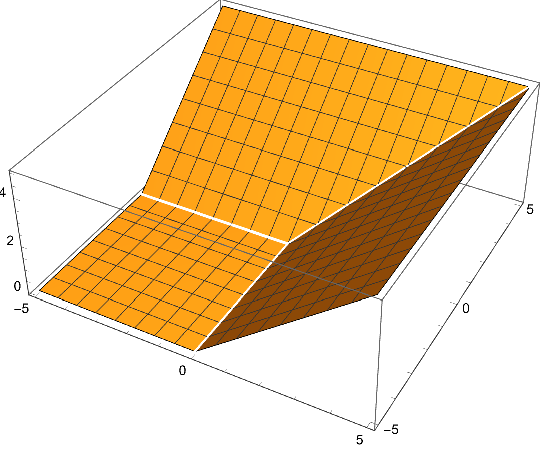
\includegraphics[width=0.3\textwidth]{figs/fig2-1-LinearTropicalPolynomial.pdf}}\quad
        \subcaptionbox{Projection onto $xy$-plane\label{fig:2.2-ProjectionLinearTropicalPolynomial}}{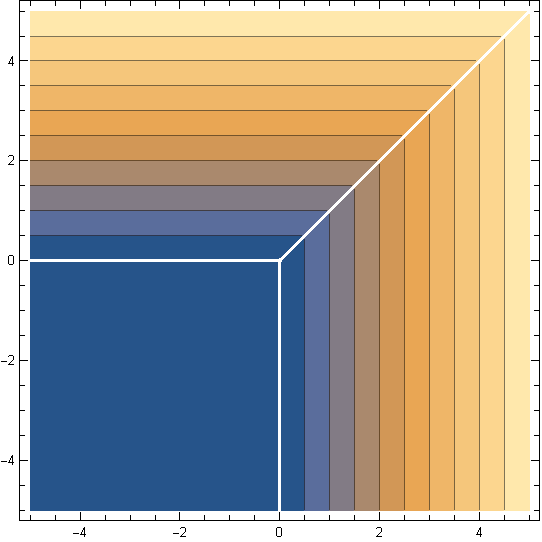
\includegraphics[width=0.25\textwidth]{figs/fig2-2-LinearTropicalPolynomialProjected.pdf}}\quad
        \subcaptionbox{Corner locus\label{fig:2.3-CornerLocus}}{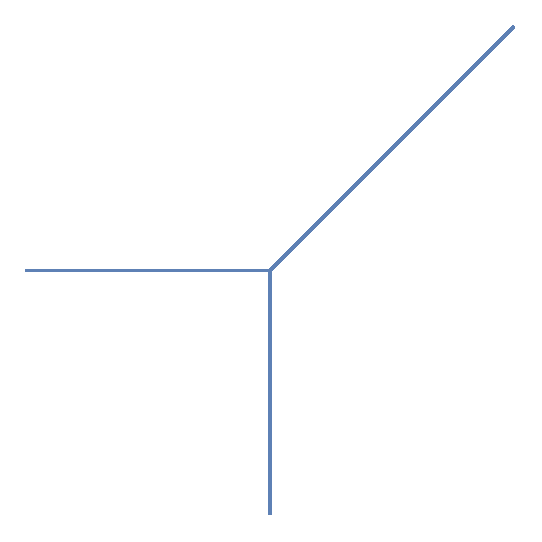
\includegraphics[width=0.25\textwidth]{figs/fig2-3-CornerLocus.pdf}}
        %\caption{This is the caption.}
        \label{fig:2.1-and-2.2-and-2.3}
    \end{figure}
    %https://mathematica.stackexchange.com/questions/169777/listplot3d-with-contours-projected-onto-the-xy-plane
    Observe that the surface is not smooth where the planes meet, this is what we will call the \emph{corner locus} or \emph{tropical hypersurface}.
    %In two variables we have a PICTURE. The polynomial $x\oplus y\oplus 0$ is actually $\max(x,y,0)$. This picture is actually the projection of the corner locus. In 3D we can visualize this better.
\end{Ex}

\begin{Def}
    The \term{tropical hypersurface} $V(\Trop(p))$ is the codimension 1 locus in $\bR^n$ where the function is non-linear (corner locus).
\end{Def}

\begin{Ex}
If we consider higher degree tropical polynomials, they will become linear in the usual sense. Consider 
$$p(x)=3x^2=3\odot x\odot x=3+x+x=3+2x$$
which is indeed linear with respect to usual sum and product.
\end{Ex}

\subsection{Valued fields}

\begin{Def}
The field of \term{Puiseux series} or rational functions over $\bC$ is $\bC(t)$ where the elements are of the form 
$$f(t)=\sum_{i=k_0}^\infty a_it^{i/n}.$$
The lower bound $k_0$ could be negative and the exponents, are rational with bounded denominators. 
\end{Def}

If we have not seen Puiseux series before it would be useful to consider a quick example:

\begin{Ex}
    Entirely by definition, consider the Puiseux series 
    $$f(t)=\sum_{i=-12}^\infty \frac{-i}{12}t^{i/6}.$$
    Expanding out the first few terms we get 
    $$\frac{12}{12}t^{-12/6}+\frac{11}{12}t^{-11/6}+\frac{10}{12}t^{-10/6}+\frac{9}{12}t^{-9/6}+\dots=t^{-2}+\frac{11}{12}t^{-11/6}+\frac{5}{6}t^{-5/3}+\frac{3}{4}t^{-3/2}+\dots$$
\end{Ex}
This field can be equipped with a valuation
$$\val_0\:\bC(t)\to\bR\cup\set{\infty},\begin{cases}
    0\mapsto \infty\\
    f\mapsto\text{order of vanishing at }0.
\end{cases}$$
This order of vanishing is the value $\al$ such that $f/t^\al$ approaches a finite non-zero value. Formally we can express this as 
$$\val_0(f)=\min\Set{\al\leq\infty\:\ \lim_{t\to0}\frac{f}{t^\al}\in\obonj{0,\infty}}.$$
The corresponding coefficient in the series expansion of $f$ for this value is called the valuation coefficient.

\begin{Ex}
    In our original example, we can see that if we divide $f$ by $t^{-2}$ (or similarly multiply by $t^2$) we get 
$$t^2f(t) = 1 + \frac{11}{12}t^{1/6} + \frac{5}{6}t^{1/3} + \frac{3}{4}t^{1/2} + \dots \xrightarrow[t\to0]{} 1 + 0 + 0 + \dots$$
If we were to divide by a lower power of $t$, say $t^{-3}$, we would get 
$$t^3f(t) = t + \frac{11}{12}t^{7/6} + \frac{5}{6}t^{4/3} + \frac{3}{4}t^{3/2} + \dots \xrightarrow[t\to0]{} 0 + 0 + \dots$$
and even if zero is a finite value, we have stated that the order of vanishing makes $f/t^\alpha$ approach a finite \textbf{non-zero} value.\par 
While on the other hand if we divide by a higher value than $-2$, say $-1$, then we get 
$$tf(t) = t^{-1} + \frac{11}{12}t^{-5/6} + \frac{5}{6}t^{-2/3} + \frac{3}{4}t^{-1/2} + \dots \xrightarrow[t\to0]{} \infty.$$
So in this case, we get a \textbf{non-finite} value. At least with this example, it gives us the intuition that the order of vanishing is a unique value.

\end{Ex}

We now ask, how does the order of vanishing behave when operating functions algebraically? What happens to the order of vanishing when you add two functions? Or when we multiply them?

\begin{Ex}
    Consider two small functions $f(t)=t^2$ and $g(t)=t^3$, then $f+g=t^2+t^3$ which has order of vanishing $2$. Observe that $2=\min(2,3)$.
\end{Ex}

In general what happens is that
$$\val_0(f+g)\geq\min(\val_0 f,\val_0 g),\word{and}\val_0(fg)=\val_0(f)+\val_0(g).$$

We can do algebraic geometry over this field! Let $\bK$ be the field of Puiseux series, if $p(x_1,\dots,x_n)\in \bK\bonj{x_1,\dots,x_n}$ then we consider the algebraic variety
$$X=V(p)=\set{\vec{x}\in\bK^n\:p(\vec{x})=0}\subseteq \bK^n.$$
Each entry of $\vec x$ is a Puiseux series we can take the valuation of. So the image through the $n$-fold valuation of $X$ will be a set in $\left(\bR\cup\set{\infty}\right)^n$. We will call the tropicalization of $X$ the image through this map. This is the tropical hypersurface for $p$.
\begin{figure}[h!]
    
\centering
\tikzset{every picture/.style={line width=0.75pt}} %set default line width to 0.75pt        

\begin{tikzpicture}[x=0.75pt,y=0.75pt,yscale=-1,xscale=1]
%uncomment if require: \path (0,300); %set diagram left start at 0, and has height of 300

%Straight Lines [id:da2454102694181276] 
\draw    (235,63) -- (299,63) ;
\draw [shift={(301,63)}, rotate = 180] [color={rgb, 255:red, 0; green, 0; blue, 0 }  ][line width=0.75]    (10.93,-3.29) .. controls (6.95,-1.4) and (3.31,-0.3) .. (0,0) .. controls (3.31,0.3) and (6.95,1.4) .. (10.93,3.29)   ;
%Straight Lines [id:da5779705315012776] 
\draw    (241,113) -- (298,113) ;
\draw [shift={(300,113)}, rotate = 180] [color={rgb, 255:red, 0; green, 0; blue, 0 }  ][line width=0.75]    (10.93,-3.29) .. controls (6.95,-1.4) and (3.31,-0.3) .. (0,0) .. controls (3.31,0.3) and (6.95,1.4) .. (10.93,3.29)   ;
\draw [shift={(241,113)}, rotate = 180] [color={rgb, 255:red, 0; green, 0; blue, 0 }  ][line width=0.75]    (0,5.59) -- (0,-5.59)   ;

% Text Node
\draw (208,53.4) node [anchor=north west][inner sep=0.75pt]    {$\bK^{n}$};
% Text Node
\draw (303,53.4) node [anchor=north west][inner sep=0.75pt]    {$(\bR\cup\set{\infty})^{n}$};
% Text Node
\draw (202,103.4) node [anchor=north west][inner sep=0.75pt]    {$V( p)$};
% Text Node
\draw (304,99.4) node [anchor=north west][inner sep=0.75pt]    {$\overline{\operatorname{val}_0( V( p))}$};
% Text Node
\draw (172,153.4) node [anchor=north west][inner sep=0.75pt]    {$\{\vec{x} :p(\vec{x}) =0\}$};
% Text Node
\draw (302,153.4) node [anchor=north west][inner sep=0.75pt]    {$\operatorname{Trop}( V( p))$};
% Text Node
\draw (210.4,98) node [anchor=north west][inner sep=0.75pt]  [rotate=-270]  {$\subseteq $};
% Text Node
\draw (328.4,98) node [anchor=north west][inner sep=0.75pt]  [rotate=-270]  {$\subseteq $};
% Text Node
\draw (229.6,127) node [anchor=north west][inner sep=0.75pt]  [rotate=-90]  {$=$};
% Text Node
\draw (346.6,127) node [anchor=north west][inner sep=0.75pt]  [rotate=-90]  {$=$};
% Text Node
\draw (172,53.4) node [anchor=north west][inner sep=0.75pt]    {$\operatorname{val}_0\:$};


\end{tikzpicture}
\caption{Diagram on the tropical hypersurface}
\label{fig:2a-diagram-trop-hypersurf}
\end{figure}

\begin{Ex}
    Consider the polynomial in $\bK\bonj{x,y}$ 
    $$p(x,y)=tx+y+t^2,$$
    then the variety is $X=\set{(x,y)\: tx+y+t^2=0}$. We can solve the equation to $y=-tx-t^2$.\par 
    If we choose $x=0$ then $y$ becomes $-t^2$. Now we take the valuation of $(0,-t^2)$ and so $(\infty,2)$ is a point in $\Trop(X)$.
\end{Ex}

\subsection{Amoebas}

Let us return to the usual stage and consider $p\in\bC[x_1,\dots,x_n]$ which defines an algebraic variety $X=V(p)\subseteq\bC^n$. Now consider the map which sends every coordinate's modulus to its logarithm in base $t$: 
$$\bC^n\to\left(\bR\cup\set{-\infty}\right)^n,\quad (z_1,\dots,z_n)\to(\log_t|z_1|,\dots,\log_t|z_n|).$$


The image of $X$ under this map, $\log_t(X)$, is the $t$-amoeba of $X$. If we take the limit as $t\to\infty$ then we get the \emph{spine} of the amoeba. 

\begin{Ex}
    When $p(x,y)=x+y-1$ then we can describe $V(p)$ via the parametrization $(x,1-x)$. So the corresponding $t$-amoeba in the real case is 
    $$\set{(\log_t|x|,\log_t|1-x|)\: x\in\bR}$$
    and we ordinarily take the limit $\lim_{t\to\infty}\frac{\log|x|}{\log t}$, we see that the functions converge to zero point-by-point. But the set is actually approaching the spine!
    \begin{figure}[h!]
        \centering
        \subcaptionbox{$X=V(x+y-1)$\label{fig:2.4-Variety}}{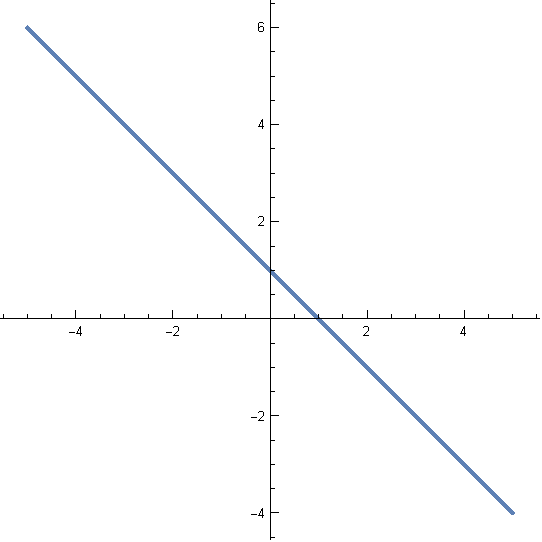
\includegraphics[width=0.25\textwidth]{figs/fig2-4-V(x+y-1).pdf}}\quad
        \subcaptionbox{$2$-amoeba of $X$\label{fig:2.5-2Amoeba}}{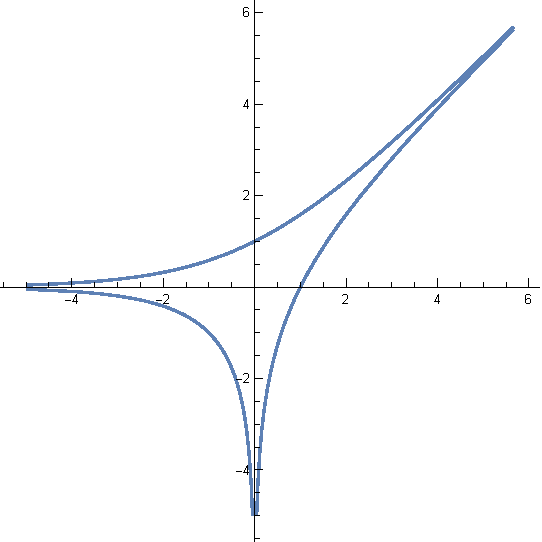
\includegraphics[width=0.25\textwidth]{figs/fig2-5-2amoeba.pdf}}\quad
        \subcaptionbox{Sequence of amoebas as $t\to\infty$\label{fig:2.6-ApproxAmoebas}}{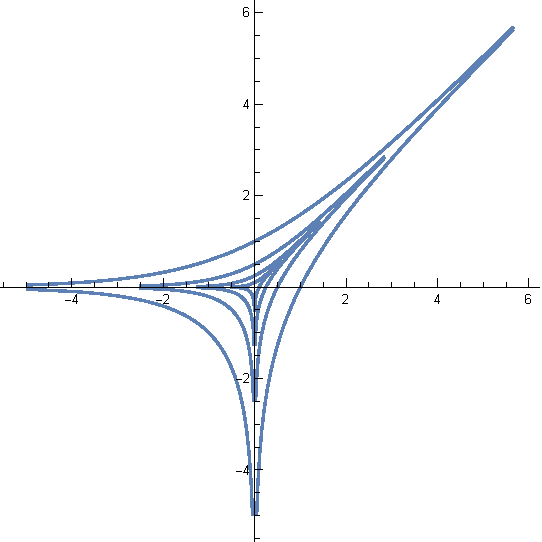
\includegraphics[width=0.25\textwidth]{figs/fig2-6-ApproximatingAmoebas.pdf}}
        %\caption{This is the caption.}
        \label{fig:2.4-thru-2.6}
    \end{figure}
\end{Ex}

Observe that the spine approaches the tropical hypersurface associated to $p$. In other words we have that the tropical hypersurface is $\lim_{t\to\infty}\log_t(V(p))$.

\subsection{Degenerations}
We may parametrize any algebraic variety with a time variable, then converting the information to a graph, edges code the information about how fast the node forms related to the length.\par
Consider a family of \red{of what, what is this family of?! Stuff? Curve in P1xP1 which eventually becomes P2?}
\begin{figure}[h!]
    \centering
    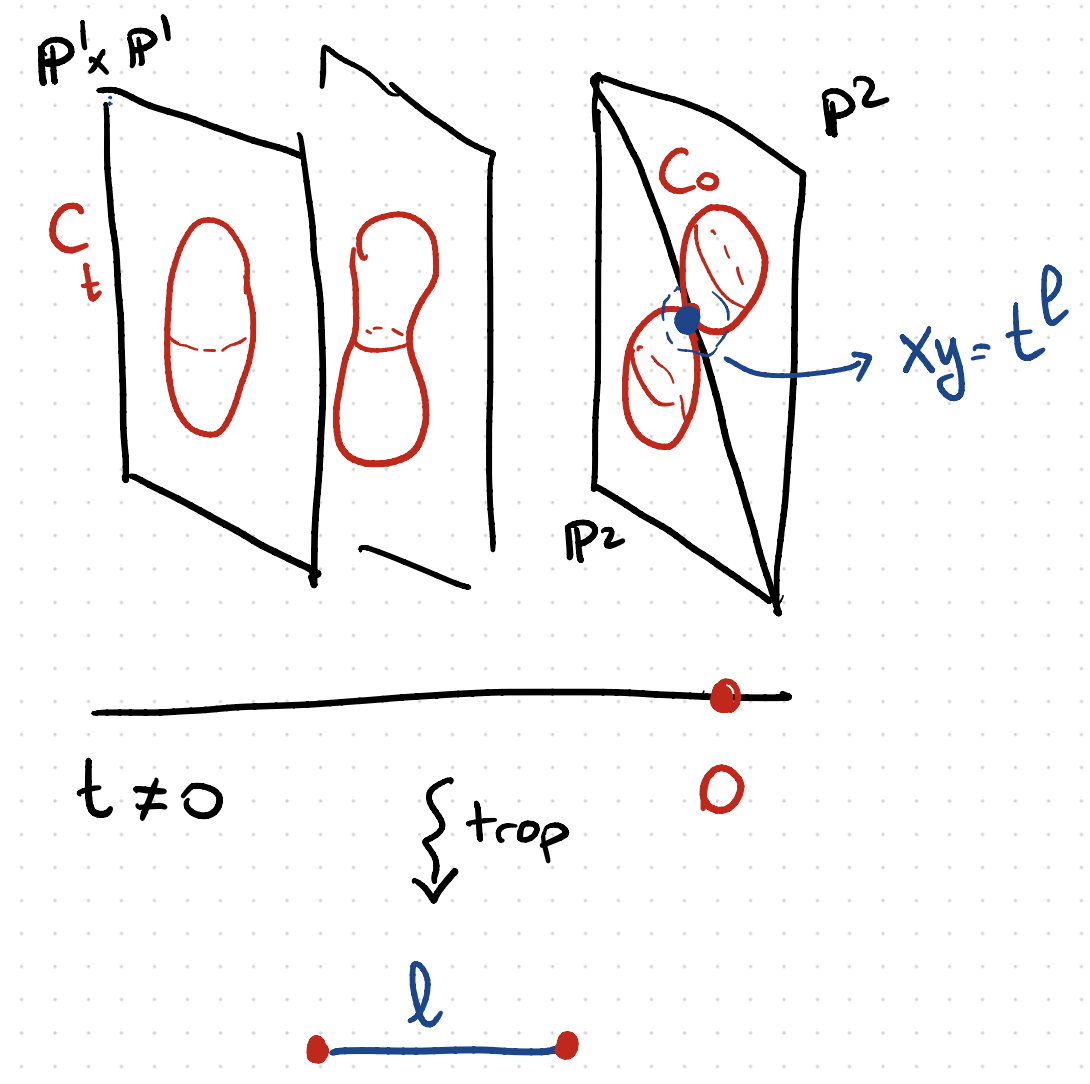
\includegraphics[width=0.5\textwidth]{figs/fig1-1.png}
\end{figure}

It is too early to understand this point of view. We will set everything up to get to it.\par 
In general, the big idea will be to explore and understand these perspectives in the case of plane curves. We want to show how they are equivalent and then recover classical algebraic geometry results in terms of tropical geometry.

\section{Day 3|20230825}

Recall that the last time we discussed the classical (25 to 30 years old) ways to get to tropical geoemtry. We now would like to answer the question
\begin{significant}
    Where do tropical numbers come from?
\end{significant}
So let us begin with an applications problem and see how the tropical numbers arise from the context of the problem.

\subsection{Tropical Arithmetics}%%%Based on TropicalNumbers.pdf

\subsubsection{Minimizing Tolls}

Consider a set of cities connected by a network of toll-ways:
\begin{figure}[h!]
    \centering
    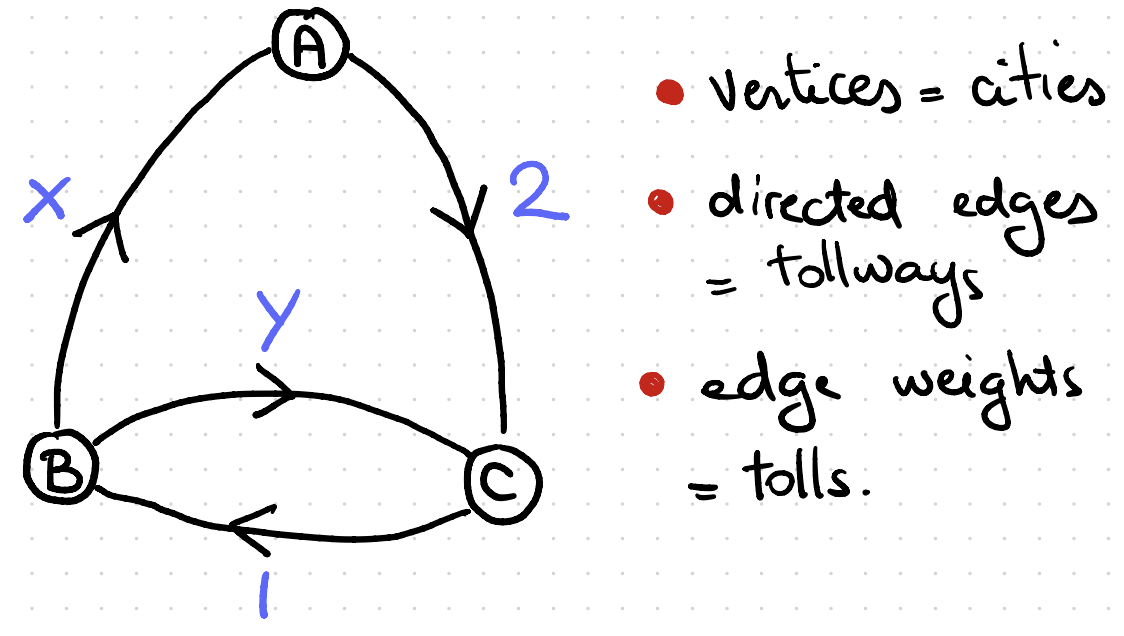
\includegraphics[width=0.5\textwidth]{figs/fig1-2.png}
\end{figure}
If we only care about minimizing toll expenses when traveling, what would be the cheapest way to go from one given city to another? Let us record the information as an incidence matrix:
$$M_{ij}=\text{price of going from city }i\text{ to city }j\text{ in at most one trip}\To M=\threebythree{0}{\infty}{2}{x}{0}{y}{\infty}{1}{0}$$
In this matrix, the rows determine the outbound city, while the columns are the destination. Each entry records the cost of a toll and tolls are considered to be infinite when the road does not exist. We can also think of $M$ as recording the cheapest toll to go from one city to another with at most one move.\par 
How would we compute the best strategy of going from city $i$ to $j$ in \emph{at most two trips}? If for example we want to find trips from $A$ to $B$ in two steps then we have three choices:
$$AAB,\quad ABB,\quad ACB.$$
The costs of each one are 
$$(0,\infty),\quad (\infty,0),\quad (2,1)$$
so we sum them and take the minimum. That will be the optimal route from $A$ to $B$ in two steps. In fact, if we relate this to the entries of the matrix $M$, we could use $M^2$. However we must redefine our basic operations as follows: 
$$+=\min,\quad\.=+$$
So we have the identification 
$$(1,2)\text{ entry of }M^2=\sum_{j=1}^{3}M_{1k}M_{k2}=\min(M_{11}+M_{12},M_{12}+M_{22},M_{13}+M_{32}).$$
In general:
\begin{align*}
    \threebythree{0}{\infty}{2}{x}{0}{y}{\infty}{1}{0}^2&=\threebythree{\min\threebyone{0+0}{\infty+x}{2+\infty}}{\min\threebyone{0+\infty}{\infty+0}{2+1}}{\min\threebyone{0+2}{\infty+y}{2+0}}{\min\threebyone{x+0}{0+x}{y+\infty}}{\min\threebyone{x+\infty}{0+0}{y+1}}{\min\threebyone{x+2}{0+y}{y+0}}{\min\threebyone{\infty+0}{1+x}{0+\infty}}{\min\threebyone{\infty+\infty}{1+0}{0+1}}{\min\threebyone{\infty+2}{1+y}{0+0}}\\
    &=\threebythree{0}{3}{2}{x}{\min(0,y+1)}{\min(x+2,y)}{1+x}{1}{\min(0,1+y)}.
\end{align*}
Observe that $1+y$ can be the minimum in the diagonal when we allow \emph{negative tolls}.
\begin{Rmk}
If we disallow negative tolls, the products $M^n$ eventually stabilize to a matrix whose entries record the cheapest way to get from one city to another in $n$ steps.
\end{Rmk}
This gives us an intuition that minimization problems correspond to linear algebra problems over $(\bT,+,\.)$ which is precisely $(\bR\cup\set{\infty},\min,+)$.

\subsubsection{Forgetting phases}

Consider the map $T_t\:\bC\to\set{-\infty}\cup\bR,\quad z\mapsto\log_t(|z|)$.
\begin{figure}[h!]
    \centering
    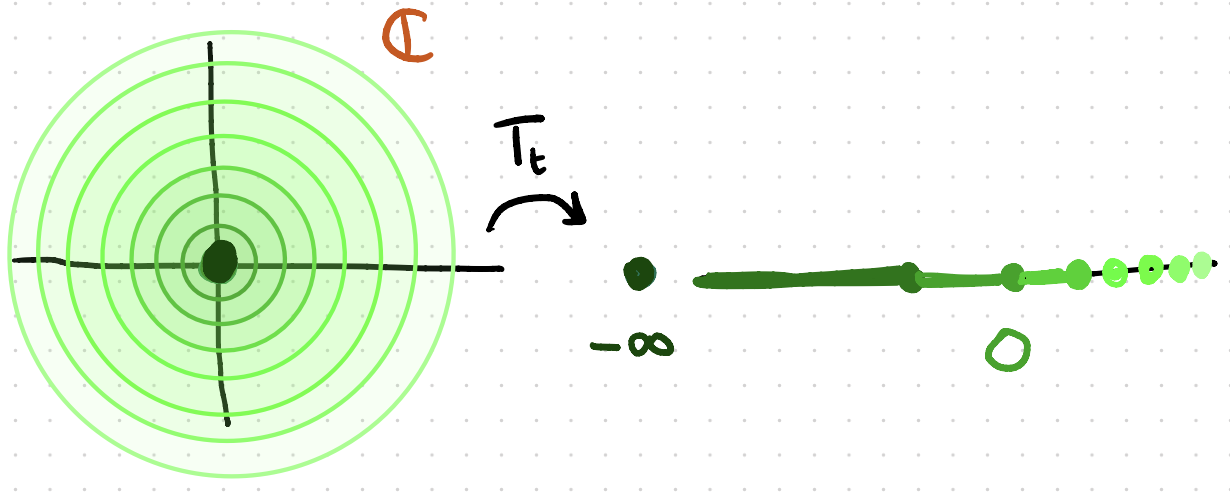
\includegraphics[width=0.5\textwidth]{figs/fig1-3.png}
\end{figure}
This map is surjective, and this we can see by checking it. Any $x\in\bR$ is 
$$T_t(t^xe^{i\te})=\log_t|t^xe^{i\te}|=\log_tt^x=x,\quad\te\in\bR.$$
This means that the inverse image of a point contains a plethora of points, in fact:
$$
\left\lbrace
\begin{aligned}
    &T_t^{-1}(x)=\set{t^xe^{i\te}}\subseteq\bC,\word{for}x\in\bR,\\
    &T_t^{-1}(-\infty)=0.
\end{aligned}
\right.
$$
With this in hand, we wish to define an exotic addition and multiplication on $\set{-\infty}\cup\bR$ using $T_t$. We will dequantize!\par 
We begin with \textbf{hyper-addition}, the output will be a subset of $\set{-\infty}\cup\bR$ so it's not a binary operation by itself. 
$$x\diamondplus_t y\:= T_t(T_t^{-1}(x)+T_t^{-1}(y))=\bonj{\log_t(|t^x-t^y|),\log_t(t^x+t^y)}.\label{problem1-hyperAddition}$$
This is an interval in $\set{-\infty}\cup\bR$, in order to make $\diamondplus_t$ into an operation we take a limit:
\begin{figure}[h!] 
    \centering
\begin{tikzpicture}[x=0.75pt,y=0.75pt,yscale=-1,xscale=1]
%uncomment if require: \path (0,300); %set diagram left start at 0, and has height of 300

%Straight Lines [id:da5156276968518897] 
\draw    (85,62.6) -- (142,62.99) ;
\draw [shift={(144,63)}, rotate = 180.39] [color={rgb, 255:red, 0; green, 0; blue, 0 }  ][line width=0.75]    (10.93,-3.29) .. controls (6.95,-1.4) and (3.31,-0.3) .. (0,0) .. controls (3.31,0.3) and (6.95,1.4) .. (10.93,3.29)   ;

%Straight Lines [id:da8224691621679702] 
\draw    (96,133) -- (144,133.38) ;
\draw [shift={(146,133.4)}, rotate = 180.46] [color={rgb, 255:red, 0; green, 0; blue, 0 }  ][line width=0.75]    (10.93,-3.29) .. controls (6.95,-1.4) and (3.31,-0.3) .. (0,0) .. controls (3.31,0.3) and (6.95,1.4) .. (10.93,3.29)   ;
%Straight Lines [id:da27001319663870027] 
\draw    (57,77) -- (57,118) ;
\draw [shift={(57,120)}, rotate = 270] [color={rgb, 255:red, 0; green, 0; blue, 0 }  ][line width=0.75]    (10.93,-3.29) .. controls (6.95,-1.4) and (3.31,-0.3) .. (0,0) .. controls (3.31,0.3) and (6.95,1.4) .. (10.93,3.29)   ;
%Straight Lines [id:da8909494911629017] 
\draw    (195,83) -- (195,120) ;
\draw [shift={(195,122)}, rotate = 270] [color={rgb, 255:red, 0; green, 0; blue, 0 }  ][line width=0.75]    (10.93,-3.29) .. controls (6.95,-1.4) and (3.31,-0.3) .. (0,0) .. controls (3.31,0.3) and (6.95,1.4) .. (10.93,3.29)   ;

% Text Node
\draw (34,53.4) node [anchor=north west][inner sep=0.75pt]    {$x\diamondplus_t y$};
% Text Node
\draw (34,123.4) node [anchor=north west][inner sep=0.75pt]    {$x\ +_{t} \ y$};
% Text Node
\draw (152,53.4) node [anchor=north west][inner sep=0.75pt]    {$x\diamondplus y=\lim _{t\rightarrow \infty } x\diamondplus_t y$};
% Text Node
\draw (152,123.4) node [anchor=north west][inner sep=0.75pt]    {$x+y=\max( x,y)$};
% Text Node
\draw (60,98.5) node [anchor=west] [inner sep=0.75pt]  [font=\scriptsize]  {$\max$};
% Text Node
\draw (114.5,59.4) node [anchor=south] [inner sep=0.75pt]  [font=\scriptsize]  {$\displaystyle\lim _{t\rightarrow \infty }$};
% Text Node
\draw (121,129.8) node [anchor=south] [inner sep=0.75pt]  [font=\scriptsize]  {$\displaystyle\lim _{t\rightarrow \infty }$};
% Text Node
\draw (197,102.5) node [anchor=west] [inner sep=0.75pt]  [font=\scriptsize]  {$\max$};


\end{tikzpicture}

\end{figure}

\begin{Rmk}
Note that $\diamondplus$ is still a hyperoperation. Its output is not a singleton \emph{only} when adding a number to itself:
$$x\diamondplus y=\begin{cases}
    \max(x,y),\quad x\neq y\\
    \bonj{-\infty,x},\quad x=y
\end{cases}$$
\end{Rmk}

Formally this process, taking a limit of a family of operations, is known as \emph{dequantization}.\par

In the case of multiplication, the process goes a lot smoother when defining it:

$$x\.y =T_t\bonj{T^{-1}(x)\.T^{-1}(y)}=\log_t\bonj{|(t^xe^{i\te})(t^ye^{i\vf})|}=\log_tt^{x+y}=x+y$$

\begin{Ex}
    Let us consider a small example like summing $2$ and $4$. Observe that 
    $$4\diamondplus_t 2=T_t(T_t^{-1}(4)+T_t^{-1}(2))=T_t\left|t^4e^{i\te}+t^2e^{i\vf}\right|$$
    and the term on the inside can be simplified to $t^{4}(e^{i\te}+t^{-2}e^{i\vf})$. $T_t$ takes that expression to
    $$4+\log_t|e^{i\te}+t^{-2}e^{i\vf}|=4+\frac{\log|e^{i\te}+t^{-2}e^{i\vf}|}{\log t}.$$
    What happens if we take the limit as $t\to\infty$? We get an independent from $t$ result! 
    The term on the right vanishes and we are left with $4=\max(4,2)$. So it got a tad bit better, but it's still a hyperoperation!
\end{Ex}

\begin{Ej}
Check how the definition of $+$ and $\.$ extend to the \emph{number} $-\infty$.
\end{Ej}

\begin{ptcb}
The point of this exercise is to operate $-\infty$ with finite numbers and itself.\par
For a finite $x$ we will find $x+(-\infty)$. This is the limit of the previous hyperoperation:
$$x\diamondplus_t(-\infty)=T_t(T_t^{-1}(x)+T_t^{-1}(-\infty))=T_t(T_t^{-1}(x)+0)=T_t(T_t^{-1}(x))=x.$$
If we let $t$ grow, the result doesn't change and so this goes according to $\max(x,-\infty)=x$.\par 
On the other hand when taking the product:
$$x\.(-\infty)=T_t\bonj{T^{-1}(x)\.T^{-1}(-\infty)}=T_t\bonj{T^{-1}(x)\.0}=T_t(0)=\log_t(0)\to-\infty$$
which is also similar to the notion of $x+(-\infty)=-\infty$.\par 
We can now proceed to operate $-\infty$ with itself:
$$(-\infty)\diamondplus_t(-\infty)=T_t(0)=\log_t(0)=-\infty=\max(-\infty,-\infty),$$
and when taking the product:
$$(-\infty)\.(-\infty)=T_t(0)\log_t(0)=-\infty=(-\infty)+(-\infty)$$
where the last sum is a sum in the usual sense.
\end{ptcb}

So, summarizing this process:
\begin{itemize}
    \item We forgot about the phase of the complex numbers and only looked at them radially. 
    \item The modulus of these numbers was scaled logarithmically.
    \item Finally we took the limit of these operations and obtained the desired (somewhat) result.
\end{itemize}
This is known as Maslov\footnote{Viktor Pavlovich Maslov (1930615-20230803)} dequantization and with this we can see $(\bT,+,\.)$ as $(\set{-\infty}\cup\bR,\max,+)$. Also, we will abbreviate $\lim_{t\to\infty}T_t$ with $T_{t\to\infty}$

\section{Interim 1|Valuations}
%%valued fields and puiseux seires

\subsection{Valuations}

In essence a valuation provides a measure of the \emph{size} (or multiplicity) of elements in a field. 

\begin{Def}
    If $K$ is a field, a \term{valuation} on $K$ is a mapping
    $$\val\:\ K\to\bR\cup\set{\infty}$$
    with the properties:
    \begin{enumerate}[i)]
        \itemsep=-0.4em 
        \item $\val(x)=\infty\iff x=0$,
        \item $\val(xy)=\val(x)+\val(y)$,
        \item $\val(x+y)\geq\min(\val(x),\val(y))$, with equality if $\val(x)\neq\val(y)$.
    \end{enumerate}
    In this case, we say that $K$ is a valued field.
\end{Def}

Previous discussion has shown us that the order of vanishing, $\val_0$ is a valuation of the field of Puiseux series $\bK$. The properties can be shown to be true by writing out two Puiseux series and showing that indeed they obey the properties.

\begin{Ej}
Verify that the field of Puiseux series, is indeed a valued field with valuation $\val_0$.
\end{Ej}

There's also a another common example coming from number theory which is the $p$-adic valuation. 

\begin{Ex}
    We first define the valuation on $\bZ$ as 
    $$v_p(a)=\max\set{k\in\bZ\:\ p^k\mid a},$$
    where $p$ is a prime number. For the rational numbers the valuation is defined as $v_p(m/n)=v_p(m)-v_p(n)$.
\end{Ex}

This valuation can be used to study the field of $p$-adic numbers which is the completion of $\bQ$ with respect to the $p$-adic absolute value $|r|_p=p^{-v_p(r)}$.

\begin{Ej}
In a similar fashion, verify that $v_p$ is a valuation over $\bQ$.
\end{Ej}

\chapter{The Tropical Numbers}

\section{Day 4|20230828}

We have seen where our ideas come from. Certain kinds of minimization problems give rise to our tropical numbers. Also by expressing complex numbers in a logarithmic scale without phase then when inducing a sum we actually get a hypersum. The way we converted into an operation is by taking a limit. Then the algebraic structure we obtained was once again the tropical numbers. Let us talk about the perspective of valued fields.
\subsection{Puiseux series}
Recall from our times in Calculus 1 that when resolving indeterminate limits, the relevant information is contained in the order of vanishing of the function.

\begin{Ex}
    Consider the limit $\lim_{t\to 0}\frac{\sin(x)}{x}=1$. Near $t=0$ we have 
    $$\sin(t)=t+o(t)\sim t^1\word{and}\frac{1}{t}=t^{-1}\word{so}t^1t^{-1}=t^0=1.$$
\end{Ex}

From this, we care to study the orders of zeroes and poles of Laurent series. In order to extend the class of functions to an algebraically closed field, we consider Puiseux series, or rational functions. We can identify Puiseux series as 
$$\bC\set{\set{t}}=\bigcup_{n\in\bN}\bC(t^{1/n}).$$
Concretely, elements here are Laurent series with rational exponents and the exponents of terms with non-zero coefficients have a common denominator. 
\begin{Ex}
    The series $\sum_{k=-37}^{\infty}t^{k/42}$ is a Puiseux series while $\sum_{k=1}^\infty t^{1/k}$ is not because the exponents keep getting smaller and smaller.
\end{Ex}
This is the most natural algebraically closed field with a \emph{canonical} valuation. This is the function:
$$\val: \bC\set{\set{t}}\to\bR\cup\set{\infty},\begin{cases}
    0\mapsto\infty\\
    t^{p/q}+\text{higher order}\mapsto p/q
\end{cases}$$

In other words the valuation sends $\sum_{k=k_0}^\infty a_kt^{q_k}$ to $q_{k_0}$.
\begin{Prop}\label{prop:PropertiesOfValuation}
For $\al,\bt\in\bC\set{\set{t}}$, the valuation enjoys the following properties:
\begin{enumerate}[i.]
    \item $\val(\al\.\bt)=\val(\al)+\val(\bt)$.
    \item $\val(\al+\bt)\geq\min(\val(\al),\val(\bt))$.
\end{enumerate}
Equality holds when $\val(\al)\neq\val(\bt)$.
\end{Prop}
So if we decide to define operations on $\bR\cup\set{\infty}$ by inducing them from the operations on $\bC\set{\set{t}}$, then we obtain
\begin{align*}
    &x\diamondplus y=\val\left(\val^{-1}(x)+\val^{-1}(y)\right),
    &x\. y=\val\left(\val^{-1}(x)\.\val^{-1}(y)\right).
\end{align*}
Now $\.$ coincides with usual addition and $+$ is the hyperoperation
$$x\diamondplus y=\begin{cases}
    \min(x,y)\word{when}x\neq y,\\
    [\min(x,y),\infty]\word{when}x=y.
\end{cases}$$
\begin{Ex}
    If we try to sum $0$ with itself, we get 
    $$0\diamondplus 0=\val\left((a_0+a_1t^{q_1}+\dots)+(-a_0+b_1t^{r_1}+\dots)\right)$$
    and this could be either $q_1$ or $r_1$ because the constant terms cancel! 
\end{Ex}
The only natural way to turn this into an operation is to define $x+y=\min(x,y)$. In conclusion, the field of Puiseux series with the order of vanishing and poles is congruent to $(\bT,+,\.)$ which in this case is $\left(\bR\cup\set{\infty},\min,+\right)$.

\subsection{The Tropical Semifield}

\begin{Def}
    The \term{tropical semifield} is $(\bT,\oplus,\odot)$ where we can choose:
    \begin{itemize}
        \item $\bT=\bR\cup\infty$, $\oplus$ to be $\min$ and $\odot$ is $+$, the min convention.
        \item $\bT=\set{-\infty}\cup\bR$, $\oplus=\max$ and $\odot=+$, the max convention.
    \end{itemize}
\end{Def}

There is a natural isomorphism between the two choices given by $x\mapsto -x$. As we have mentioned, different contexts may be more natural than the other when using certain conventions. We will typically use the $\max$ convention. 

\begin{Prop}
The following algebraic properties hold for $(\bT,+,\.)$:
\begin{enumerate}[i)]
    \itemsep=-0.4em
    \item $0_\bT=-\infty$.
    \item $1_{\bT}=0$.
    \item $x\oplus y=0_\bT$ only has the solution $x=y=0_\bT$. This means that only $-\infty$ has an additive inverse.
    \item Addition is idempotent: $x\oplus x=x$.
    \item Every non-zero element has a multiplicative inverse: $1/x=-x$.
\end{enumerate}
\end{Prop}

\begin{ptcbp}
    \begin{enumerate}[i)]
        \itemsep=-0.4em
    \item Observe that $x\oplus0_\bT=\max(x,-\infty)=x$.
    \item $x\odot 1_\bT=x+0=x$.
    \item $x\oplus y=0_\bT\iff \max(x,y)=-\infty\To x=y=-\infty$.
    \item $x\oplus x=\max(x,x)=x$.
    \item $x\.(1/x)=x+(-x)=0=1_\bT$.
\end{enumerate}
\end{ptcbp}
Observe that it is not possible to adjoin formal additive inverses. Suppose that for $x\in\bT$ there exists a $y$ such that $x+y=0_\bT$, then 
$$(x\oplus x)\oplus y=x\oplus y=0_\bT\word{and}x\oplus (x\oplus y)=x\oplus 0_\bT=x\word{but}x\neq 0_\bT.$$
This means that any invertible element necessarily has to be $-\infty$.

\begin{Ej}[2-]
Which other algebraic properties do these operations enjoy? We have claimed for example that $\oplus$ is associative. Prove this.\par 
Are the operations commutative? Do they distribute with respect to each other?
\end{Ej}

\begin{ptcb}
Let us assume without losing generality that 
$$x<y<z$$
and then 
\begin{align*}
    &x\oplus (y\oplus z)=\max(x,\max(y,z))=\max(x,z)=z\\
    &(x\oplus y)\oplus z=\max(\max(x,y),z)=\max(y,z)=z
\end{align*}
which shows us that $\oplus$ is associative. We can see that it's commutative by realizing that $\max$ is also commutative.\par 
Finally we ask if distribution occurs, but let us observe first that 
$$y<z\To x+y<x+z,$$
now we can see that 
\begin{align*}
&x\odot(y\oplus z)=x\odot y\oplus x\odot z\\
\iff &x+\max(y,z)=\max(x+y,x+z)\\
\iff &x+z=x+z
\end{align*}
which proves distributivity. Also it is not necessary to check distribution on the other side as our operations are commutative.
\end{ptcb}

\begin{Prop}[Weird Fun Facts]
Recall that the usual Pascal Triangle is built by adding the previous two elements to get the next one. In the tropical case we have 
$$
%https://tex.stackexchange.com/questions/17522/pascals-triangle-in-tikz
\begin{tikzpicture}
    \foreach \n in {0,...,2} {
      \foreach \k in {0,...,\n} {
        \node at (\k-\n/2,-\n) {$1_\bT$};
      }
    }
    \end{tikzpicture}
    \word{\raisebox{2.5em}{=}}%tex.se/47016
    \begin{tikzpicture}
        \foreach \n in {0,...,2} {
          \foreach \k in {0,...,\n} {
            \node at (\k-\n/2,-\n) {$0$};
          }
        }
        \end{tikzpicture}
    $$
    and this extends downwards with the same pattern.\par 
    In the case of the tropical binomial theorem, we have a ``freshman's dream'' type of identity:
    $$(x\oplus y)^n=x^n\oplus y^n.$$

Observe that in other words, what the binomial theorem is telling us is a restatement of the identity $n\max(x,y)=\max(nx,ny)$.
\end{Prop}

\begin{Ej}[2]
Recall that the coefficients in the expansion for the binomial theorem are the corresponding elements in the rows of the Pascal Triangle. Verify if the coefficients agree in the tropical case for the binomial theorem.
\end{Ej}

\begin{ptcb}
We must verify that the coefficient of every monomial in the expansion of $(x\oplus y)^n$ does match the $n^{\text{th}}$ row of Pascal's triangle. To that effect note that 
\begin{align*}
    (x\oplus y)^n&=(x\oplus y)\odot(x\oplus y)\odot\dots\odot(x\oplus y)\\
    &=x^n\oplus x^{n-1}y\oplus\dots\oplus xy^{n-1}+y^n\\
    &=x^n\oplus y^n
\end{align*}
and in the second line, remember we would usually have $\binom{n}{k}$ terms of the form $x^ky^{n-k}$. However, as addition is idempotent here, all those terms become just one term.\par 
Also, observe that the coefficient (tropically) multiplying each term is $1_\bT$. This is because multiplication by one is just adding by zero. So it is indeed the case that all coefficients in the binomial expansion are $1_\bT$.\par 
Finally observe that for any $k$, $kx+(n-k)y\leq\max(nx,ny)$ which means that the only terms that survive are the power $n$ monomials in the expansion. 
\end{ptcb}


\subsubsection{The Optimal Assignment Problem}

Suppose we have $n$ jobs for $n$ workers. Each worker can only work one job and once the job is taken, no one else can do it. We wish to assign a job to each worker in order to maximize our company's profit.

\begin{Ex}
    As a little example consider Alice and Bob's hydroponics farm. When working with the weeds Alice produces $5$ credits while working with the water she produces $6$. On the other hand Bob produces $3$ and $5$ respectively.\par 
    It is easy to see that Alice should be assigned to to the weed and Bob to the water in order to maximize. But let us apply what we know with tropical arithmetics.\par 
    Call 
    $$M_{ij}=\text{amount of credits work }i\text{ produces when doing job }j.$$
    Then we can summarize the previous information in a matrix 
    $$M=\twobytwo{5}{6}{3}{5}$$
    and if we take the tropical determinant (which is really a permanent since we lack subtraction) we get
    $$\Trop\det M=5\.5+6\.3=\max(5+5,6+3)=10$$
    which is the maximal profit we can make by assigning our workers.
\end{Ex}

\begin{Ej}
    Do the following:
    \begin{enumerate}[i)]
        \itemsep=-0.4em
        \item[(1-)] Construct a $3\x3$ matrix with non-permuted entries such that there's more than one possible assignment for the optimal jobs.
        \item[(1)] Use the combinatorial definition of permanent to show that the tropical determinant of $M$ is indeed the maximal profit. \hint{The definition of permanent is the same as the determinant but without the $(-1)^{\sgn\sg}$.}
        \item[(1)] Assuming you know the tropical determinant of a matrix, devise a way to identify one job combination which reaches the optimum value. \aside{Actually! It is not necessary to know the value of the determinant.}
    \end{enumerate}
\end{Ej}

\begin{ptcb}
    \begin{enumerate}[i)]
        \itemsep=-0.4em
        \item Consider a matrix $A\in \bR^{3\x3}$. For a given $n\in\bN$, the profit, we may build an infinite family of matrices which satisfy the required conditions.\par 
        The conditions our matrix must satisfy are sums of permuted entries.\par 
        In this case the solution is given by $5$ parameters including the profit:
        $$(n-f-h,n-g-g,n-f-g-h+i,f+g-i,f+h-i,f,g,h,i)$$
        so a valid matrix could be 
        $$\threebythree{1}{3}{1}{3}{5}{3}{2}{4}{2}.$$
        \item The permanent by definition is 
        $$\bigoplus_{\sg\in S_n}\bigodot_{i=1}^n M_{i\sg_i}=\max_{\sg\in S_n}\left(\sum_{i=1}^n M_{i\sg_i}\right).$$
        What the last expression says is, out all the possible permutations, which is the highest sum over all possible job assignments. So the permanent will indeed find the maximal profit.
        \item We can proceed with a greedy algorithm. Row by row, choose the largest element. Then eliminate the column the found element was in and repeat the process.\par 
        For example, pick $A_{1k}=\max(\text{row }1)$, then throw out column $k$ and repeat the process with the $(1,k)$ minor of $A$.\aside{This doesn't actually prove that the greedy algorithm works.} 
    \end{enumerate}
\end{ptcb}

\begin{Rmk}
Observe that the first problem can be solved in any dimension $d$, because in total we have $2d$ equations while having $d^2$ indeterminates. As $2d<d^2$ for $d\geq 2$, we have that the problem will always be under-determined. So there's always more than one possible optimal assignment. 
\end{Rmk}

We now have another question, 
\begin{significant}
    Is there an instance where the greedy algorithm fails to find an optimal assignment for the jobs?
\end{significant}

\begin{Ej}[5]
Prove or disprove, the greedy algorithm will find an optimal assignment for the jobs given the conditions above. You may assume to know the value of the permanent of the matrix.
\end{Ej}
\section{Day 5|20230830}

The last time we talked about the algebraic structure of the value group of the Puiseux series. We now have plenty of motivation of why would we define the tropical numbers. 

\subsection{Tropical Polynomials and Roots}

An univariate,tropical, (Laurent) monomial is equivalent to an affine linear function with integer coefficients. Such a monomial is an expression of the form 
$$a\odot x^{\odot m},\quad a\in\bT,\quad m\in\bZ.$$

\begin{Ex}
    We have for example:
    $$5x^2\otto 5+2x,\quad 2x^{-3}\otto 2-3x.$$
    The second one is a Laurent monomial because of the negative power. Also consider $\sqrt 5\odot x^{\odot 3}$ which corresponds to $y=\sqrt{5}+3x$. Notice how the slope is always an integer, meanwhile the translation can be any number.
\end{Ex}

An univariate tropical (Laurent) polynomial is a finite sum of monomials which give rise to a \emph{convex}, continuous, piecewise, affine linear function with integer slopes. 

\begin{Ex}
    Consider the function $-5\odot x^{\odot2}\oplus(-2)\odot x^{\odot-3}\oplus 0$ which corresponds to 
    $$\max(-5+2x,-2-3x,0).$$
    If we graph this functions we obtain
    \begin{figure}[h!]
        \centering
        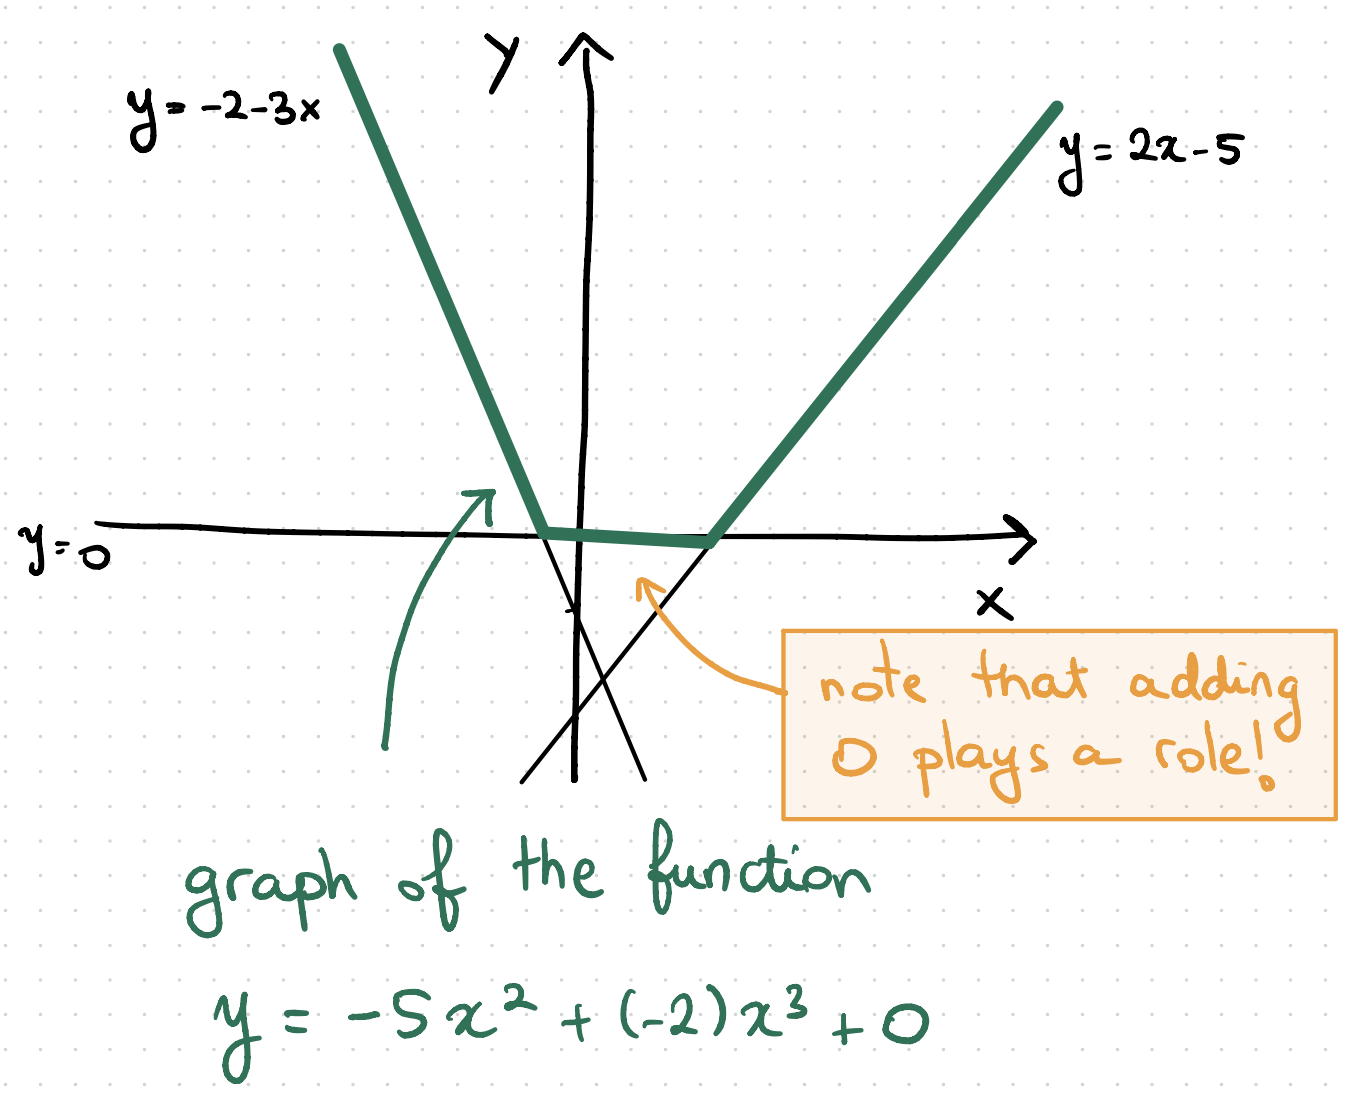
\includegraphics[width=0.5\textwidth]{figs/fig3-1RenzoNotes3.png}
        %\caption{This is the caption.}
        \label{fig:3.1-ConvPLFunc}
    \end{figure}
    Observe that this function is indeed convex, and fulfills all of the previous properties from before. 
\end{Ex}

In fact the map from $\bT[x]$ to convex, affine piecewise linear functions with \emph{finitely} many distinct regions of linearity is surjective. If we don't want to take the finiteness condition into consideration, we have to amplify the domain to tropical Laurent series.\par 
A small measure of care should be taken because there are multiple tropical polynomials which map to the same function.

\begin{Ex}
    Consider the functions 
    $$p_1=x+\frac{1}{x}+0,\quad p_2=x+\frac1x-2.$$
    When converting we get 
    $$\max(x,-x,0),\quad\max(x,-x,-2)$$
    which produce $|x|$ in both cases.
    \begin{figure}[h!]
        \centering
        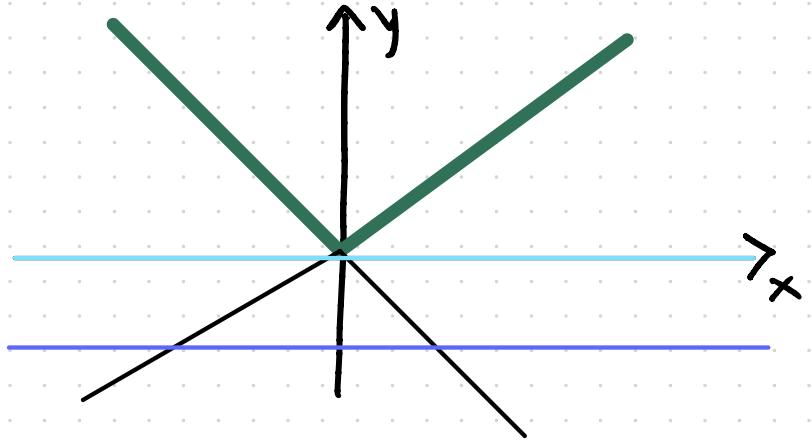
\includegraphics[width=0.5\textwidth]{figs/fig3-2RenzoNotes3.png}
        \caption{Failure of injectivity as both functions map to $|x|$ with $y=0$ and $y=-2$ shown.}
        \label{fig:3.2-InjectivityFailure}
    \end{figure}
    Adding something which is smaller than the minimum value of the function doesn't change it in general. It also doesn't have to be a constant in general. In the previous example, the the monomial $(-4)\odot x^{\odot 1}$ is smaller than any of the linear functions, so adding it changes nothing.
\end{Ex}

To talk about the roots, we will start with a purely combinatorial definition. 

\begin{Def}
    Given a polynomial $p\in\bT[x]$ of degree $d$ we say the following:
    \begin{itemize}
        \item $-\infty$ is a root of $p$ if the slope of the piecewise linear function is non-zero for $x\ll 0$.
        \item $x_0\in\bR$ is a root of $p$ if $p'(x_0)$ is undefined. Observe that the derivative is undefined only when there's a change in slope.
    \end{itemize}
    We say that the \term{multiplicity} of $x_0$ is the difference between slopes across $x_0$. If $-\infty$ is a root, then its multiplicity is equal to the slope of the associated function for $x\ll 0$.
\end{Def}

\begin{Ex}
    Consider the polynomial $x^{\odot2}\oplus1\odot x^1\oplus 0=\max(2x,x,0)$.
    \begin{figure}[h!]
        \centering
        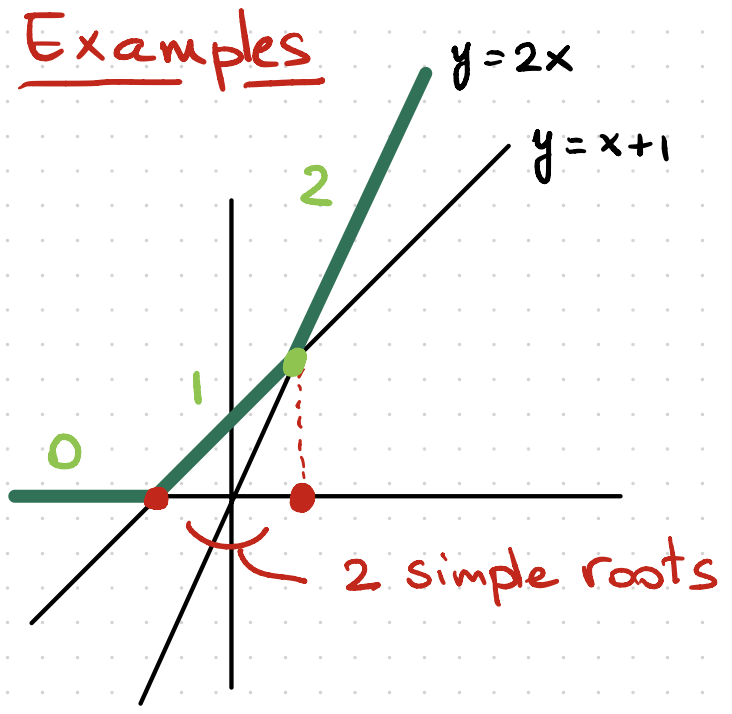
\includegraphics[width=0.5\textwidth]{figs/fig3-3SimpleFiniteRootsTropicalPolynomial.png}
        %\caption{}
        \label{fig:3.3-SimpleFiniteRoots}
    \end{figure}
    We can see that there are changes in slope at $x_1=-1$ and $x_2=1$. The number of roots coincides with the degree of the polynomial as in the usual sense.
\end{Ex}

\begin{Ex}
    Let's remove the zero, recall zero isn't the additive identity, so the polynomial we have is $x^{\odot2}\oplus1\odot x^1=\max(2x,x)$.
    \begin{figure}[h!]
        \centering
        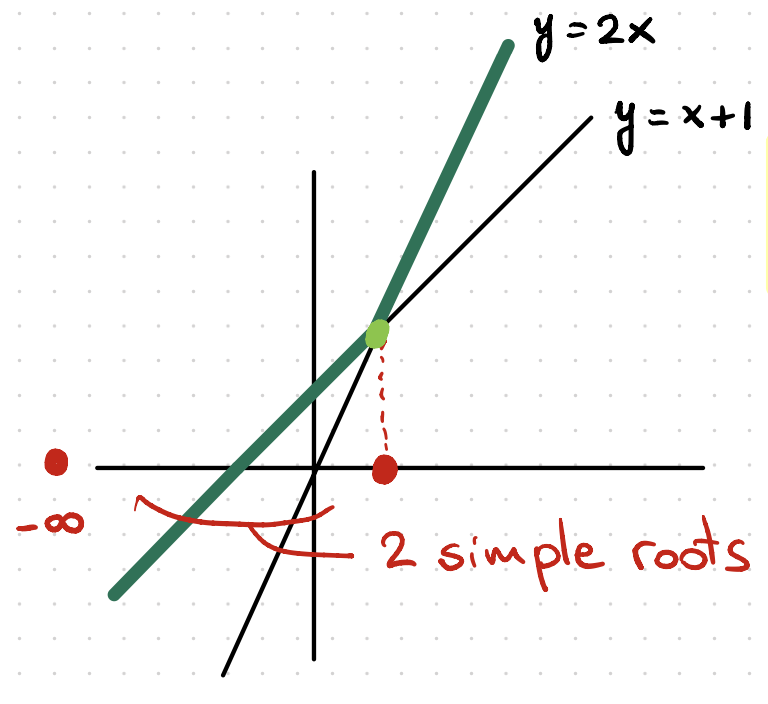
\includegraphics[width=0.5\textwidth]{figs/fig3-4SimpleRootsTropicalPolynomial.png}
        %\caption{}
        \label{fig:3.4-OneFiniteRootOneInfiniteRoot}
    \end{figure}
    Now one of the roots is still $x=1$, but remember that if the slope is non-zero when $x\ll 0$, then $-\infty$ is a root of $p$. This is the case here because the slope is $1$ as $x\to-\infty$. Once again there's two roots $x_1=-\infty$ and $x_2=1$.
\end{Ex}

\begin{Ex}
    Let us change a sign in a coefficient, take $x^2-1\.x^1+0$. But what is tropical subtraction? It's not that, let's convert this slowly into what it's supposed to be:
    $$x^2-1\.x^1+0=(x\.x)+(-1)\.x+0=(2x)+(x+(-1))+0=\max(2x.x-1,0).$$
    \begin{figure}[h!]
        \centering
        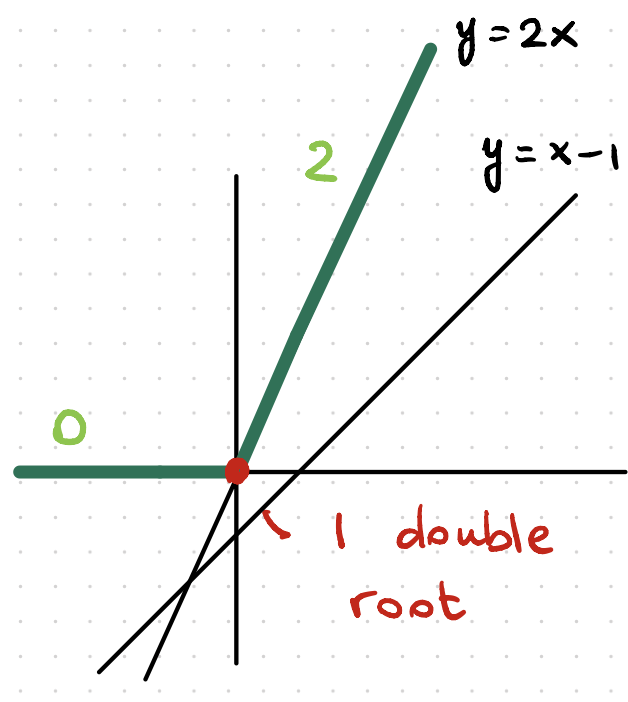
\includegraphics[width=0.5\textwidth]{figs/fig3-5DoubleRootTropicalPolynomial1.png}
        %\caption{}
        \label{fig:3.5-DoubleRoot1}
    \end{figure}
    Observe that because the line $y=x-1$ is below our graphs, it doesn't interfere with the calculation of zeroes. So the only place where there occurs a change in sign is $x=0$. The slope on the right is $2$ and on the left is $0$ so the multiplicity is $2-0=2$.
\end{Ex}

\begin{Ex}
    In a similar fashion, $x^2+0$ also has a double root at $x=0$.
    \begin{figure}[h!]
        \centering
        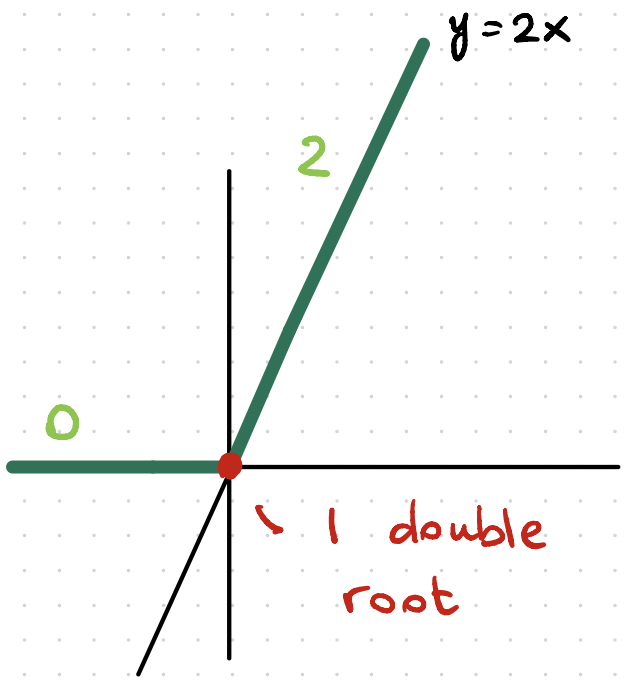
\includegraphics[width=0.5\textwidth]{figs/fig3-6DoubleRootTropicalPolynomial2.png}
        %\caption{}
        \label{fig:3.6-DoubleRoot6}
    \end{figure}
    There is only one change in slope once again at $x=0$ and the difference in slopes is $2$.
\end{Ex}

\begin{Lem}
For a tropical polynomial $p$, a finite $x_0$ is a root of $f$ if and only if when we write the function as a $\max$ of linear functions, at $x_0$ the maximum value is obtained at least twice.\par 
The multiplicity of the root is equal to the difference in the two extremal positions where the $\max$ is attained.
\end{Lem}

This should be more or less obvious. Being a root means that we are an intersection of two lines which are above all the others. It's pretty useful to have this notions around.

Questions arise:
\begin{significant}
    Which functions have only one simple zero at $-\infty$? What would a function with an order 2 zero at $-\infty$ look like?
\end{significant}

\begin{Ej}
    Do the following:
    \begin{itemize}
        \item[(5)] Is it possible for a function to have only a simple zero at $-\infty$? Provide an example of function with one simple zero at $-\infty$ or prove that such function cannot exist. 
        \item[(5)] Do functions with zeroes at $-\infty$ have infinite order at such zero or is it arbitrarily high? If a function has a finite order zero at $-\infty$ provide an example of one with a double zero at $-\infty$. Else, prove that such functions have infinite order at that zero.
    \end{itemize}
\end{Ej}

\section{Day 6|20230901}

How do we know that the notions of roots are natural or useful?

\subsection{Factorization of Tropical Polynomials}

Suppose a polynomial $p\in\bT[x]$ has roots $a_k$ with multiplicity $m_k$. Then we may factor $p$ as a product of linear polynomials 
$$p(x)=c_0\bigodot(x\oplus a_k)^{m_k}.$$
This $p$ is the affine piecewise-linear function, not the formal object. And so, in a sense, $\bT$ is algebraically closed. But instead of proving this, we will sketch the proof to get an idea of how things \emph{work} with a couple of examples.\par 
The idea of the proof is that we check that product does define a P.L. function with the right slopes and then $c_0$ gives the translation factor.
\begin{Ex}
First lets deal with the case where $-\infty$ is not a root. Consider the polynomial 
$$p(x)=(-1)\oplus(-1)\odot x\oplus(-4)\odot x^4=\max(-1,x-1,4x-4).$$
Remember, as in the case of real polynomials, the square and cube terms are still there. The coefficient that foes along them is just $-\infty$. We can graph the polynomial in order to see the roots:
\begin{figure}[h!]
    \centering
    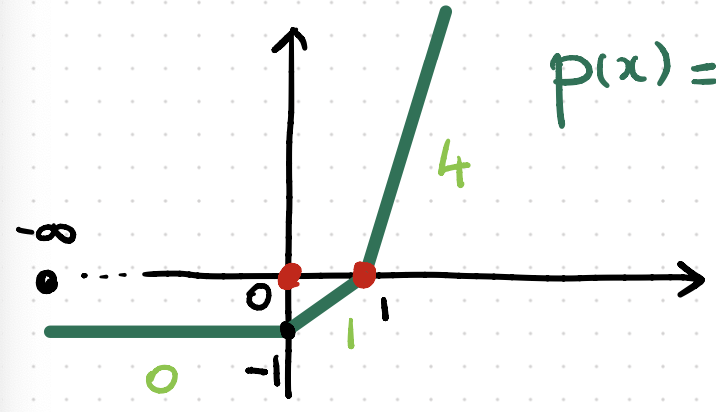
\includegraphics[width=0.5\textwidth]{figs/fig4-1-InfinityNotRoot.png}
    \caption{Graph of $p(x)$ with roots shown}
    \label{fig:4.1-InfinityNotRoot}
\end{figure}
The points where there is a change in slope are $a_1=0$ and $a_2=1$. Then their multiplicities are $1-0=1$ and $4-1=3$ respectively. We may write $p$ as 
$$p(x)=c_0\odot(x\oplus 0)\odot(x\oplus 1)^{3}=c_0+\max(x,0)+\max(3x,3).$$
Whatever function we have, we can write as the sum of three terms. So let us subdivide the tropical line in order to see which terms goes where.
\begin{table*}[h!]
    \centering
    %\arraystretch{1.3}
    \begin{tabular}{rrrr}\toprule
        $x\leq 0$ & $0\leq x\leq 1$ & $1\leq x$\\ \midrule
        $c_0$& $c_0$&$c_0$\\
        $0$&$x$ & $x$\\
        $3$& $3$ & $3x$\\ \midrule
        $c_0+3$&$c_0+3+x$&$c_0+4x$\\
   \bottomrule
    \end{tabular}
    \legend{Behavior of $p(x)$ across $\bT$}
    \end{table*}
    The constant can be determined by plugging in $x=-\infty$. We can see that 
    \begin{align*}
        p(-\infty)&=(-1)\oplus(-1)\odot (-\infty)\oplus(-4)\odot (-\infty)^4=-1\\
        &=c_0\odot(-\infty\oplus 0)\odot(-\infty\oplus 1)^3=c_0\odot0\odot 1^{\odot 3}.
    \end{align*}
    This gives us the equation $c_0+0+3=-1$ which leads us to $c_0=-4$. With this we verify that 
    $$p(x)=\begin{cases}
        -1&x\leq 0\\
        x-1&0\leq x\leq 1\\
        4x-4&1\leq x
    \end{cases}$$
    So in this case $c_0=p(-\infty)-\sum m_ka_k\in\bR$.
\end{Ex}

\begin{Ex}
    We now explore the case where $-\infty$ is a root or a pole. The argument will essentially be the same with a small modification.\par 
    Consider the function $\frac{1}{x}\oplus x$.
    \begin{figure}[h!]
        \centering
        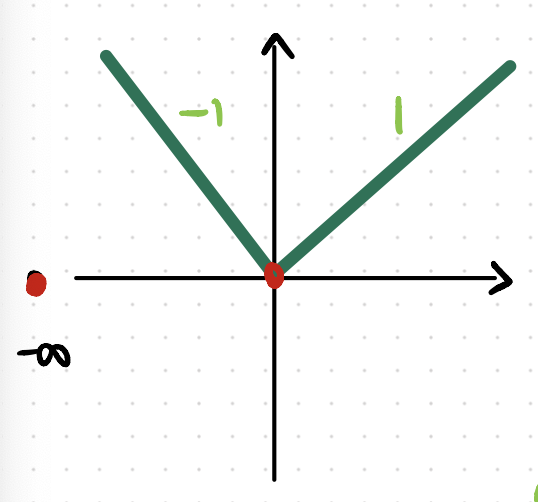
\includegraphics[width=0.5\textwidth]{figs/fig4-2RootAndPoleProof.png}
        %\caption{}
        \label{fig:4.2-RootAndPoleProof}
    \end{figure}
    We have $-\infty$ as a pole of order $1$ and $0$ is a root of order $1-(-1)=2$. So this can be factored as 
    $$p(x)=c_0\odot(x^{-1})\odot(x+\oplus 1)^2$$
    and even if $-\infty$ doesn't give us a particular value for the function, we can still find $c_0=0$ from the equation $p(0)=0$.\par 
    If on the other hand we have a negative slope then we have a zero at $-\infty$. Consider the function $p(x)=x+x^2$:
    \begin{figure}[h!]
        \centering
        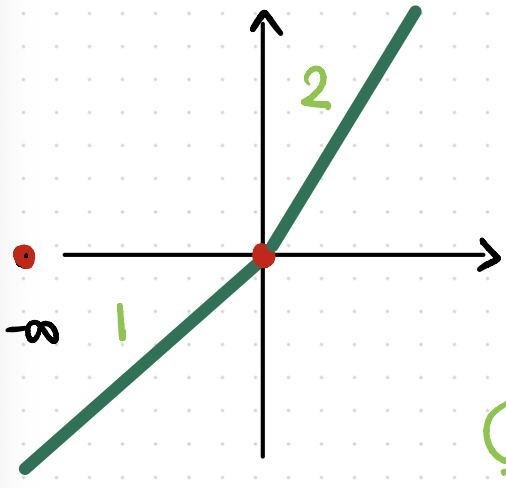
\includegraphics[width=0.5\textwidth]{figs/fig4-3RootsForProof.png}
        %\caption{}
        \label{fig:4.3-RootsForProof}
    \end{figure}
    This function has two simple roots at $-\infty$ and $0$. We may factor it as 
    $$p(x)=c_0\odot(x\oplus-\infty)\odot(x\oplus 0)$$
    and even if $p(-\infty)=-\infty$ we can plug in $0$ to get $0$ back in order to get $c_0=1$.
\end{Ex}

\subsection{Correspondence Theorems}
Recall the maps
$$
\left\lbrace 
\begin{aligned}
    &T_t\: \bC\to\bT\quad(\text{with }\max),\\
    &\val\: \bC\set{\set{t}}\to\bT\quad(\text{with }\min).
\end{aligned}
\right.
$$
If we consider a polynomial 
$$p(X)\in\bC[X]\word{or}p(x)\in\bC\set{\set{t}}[X]$$
then we can produce a tropical polynomial as follows:

\begin{enumerate}[i.]
    \item Apply $T_t$ or $\val$ to the coefficients, and
    \item Perform tropical operations.
\end{enumerate}

We expect that if $r\in\bC$ or $r\in\bC\set{\set{t}}$ is a root of $p$, then $\lim_{t\to\infty}T_t(r)$ will be a root of the new polynomial.\par
Or the other way around, given $p\in\bT[x]$, we can lift the coefficients to $\bC$ or the Puiseux series via the above maps. We can find the roots of the corresponding polynomials in $\bC[x]$ or $\bC\set{\set{t}}[x]$ and then the image of those roots via $T_t$ or $\val$ are the tropical roots of $p(x)$.

\begin{Ex}
    Consider the polynomial $p(x)=2\odot x\oplus3\in\bT[x]$. We wish to construct a polynomial in $\bC[x]$ which tropicalizes to $p$. Take the polynomial 
    $$q(x)=t^2X+t^3\in\bC[x],\quad t>0$$ 
    We could certainly add phase as $e^{i\te}$ to the $t^k$'s, but that won't change anything. Taking the logarithm of the coefficients we get 
    $$t^2\mapsto 2\word{and}t^3\mapsto 3.$$ 
    Then switching the operations to tropical operations we have
    $$t^2X+t^3\xrightarrow[]{\Trop}2\odot X\oplus 3$$ 
    which was our original polynomial $p$.\par 
    Additionally if we solve the equation $q=0$ we obtain the root $X=-t^3/t^2=-t$. Now $\log_t|-t|=1$. Lo and behold, this is the same root of $p(x)$. 
    \begin{figure}[h!]
        \centering
        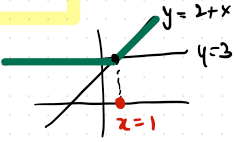
\includegraphics[width=0.5\textwidth]{figs/fig4-4CorrespondenceRoots1Example.png}
        \caption{Root of $p(x)$ in correspondence with $-t$ of $q(x)$}
        \label{fig:4.4-CorrespondenceRoots1Example}
    \end{figure}
\end{Ex}

We should be skeptical because this was only an example of a linear polynomial. Lets increase the degree and see what happens. Eventually this correspondence must be shown to hold in its entirety.

\begin{Ex}
    Consider the polynomial
    $$q(X)=X^2+t^2X+1\in\bC[X]\xrightarrow[]{\Trop}p(x)=x^2\oplus 2\odot x\oplus 0.$$
    We can identity the roots of $p$ as $-2$ and $2$. However, we may find it difficult to interpret the roots of $q$ as roots of $p$. Observe that using the quadratic formula we may derive those to be:
    $$X_{1,2}=\frac{-t^2}{2}\pm\frac{\sqrt{t^4-4}}{2}=\frac{-t^2}{2}\left(1\pm\sqrt{1-\frac{4}{t^4}}\right).$$
    Even if taking the logarithm seems hard, we are not interested in the logarithm itself, just the limit! Observe that 
    $$\lim_{t\to\infty}\log_t\left|\frac{-t^2}{2}\left(1+\sqrt{1-\frac{4}{t^4}}\right)\right|=2+\lim_{t\to\infty}\frac{1}{\log(t)}\log\left|\frac{1}{2}\left(1+\sqrt{1-\frac{4}{t^4}}\right)\right|$$
    and the quantity on the right tends to $1/\infty$ which collapses to zero and then the logarithm only has $1$ as its argument. So overall we find one our original roots: $2$! The next limit has a different sign so it is not as direct. We may calculate that limit as follows:
    $$\lim_{t\to\infty}\log_t\left|\frac{1}{2}\left(1-\sqrt{1-\frac{4}{t^4}}\right)\right|\approx\lim_{t\to\infty}\log_t\left|\frac{1}{2}\left(1-\left(1-\frac{4}{2t^4}\right)\right)\right|=\lim_{t\to\infty}\log_t\frac{1}{t^4}=-4.$$
    So for the negative root we would actually obtain $2-4=-2$ which is the other root of our polynomial.
    \begin{figure}[h!]
        \centering
        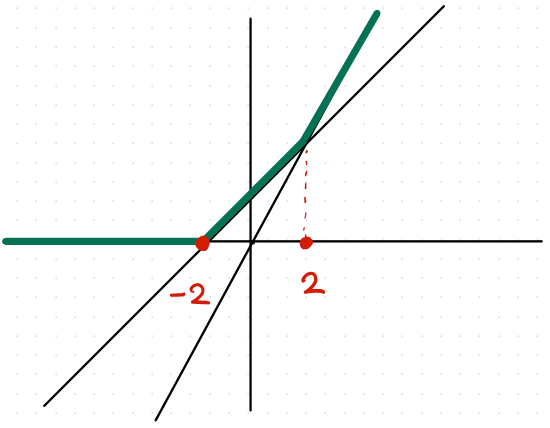
\includegraphics[width=0.5\textwidth]{figs/fig4-5CorrespondenceRoots2Example.png}
        \caption{Indeed the roots of $q$ correspond with $p$'s}
        \label{fig:4.5-CorrespondenceRoots2Example}
    \end{figure}
\end{Ex}

\section{Interim 2}

\begin{Def}
    If $q(x)=\sum a_kx^k\in\bC[X]$ or $\bC\set{\set{t}}[x]$, then the \term{tropicalization} of $q$ is 
    $$\Trop(q)=\sum T_{t\to\infty}(a_k)x^k$$
    or respectively with the valuation. In this case we omit the notation for tropical operations but the sum and product are tropical.
\end{Def}

\begin{Th}
For a polynomial $q$, $r_k$ is a root of $q(x)$ with multiplicity $m_k$ if and only if $T_{t\to\infty}(r_k)$ is a root of $\Trop(q)$ of multiplicity $m_k$.
\end{Th}

In the univariate case, we may prove the theorem using the following lemmas.

\begin{Lem}
$\Trop$ is a multiplicative function on polynomials. That is
$$\Trop(pq)=\Trop(p)\Trop(q)\word{for}p,q\in\bC[x].$$
\end{Lem}

\begin{Lem}
The roots of $\Trop(p)\Trop(q)$ are the union of the roots of the factors. If a root is repeated then the multiplicities are added.
\end{Lem}

\begin{Ej}[2]
Prove the preceding lemmas and then conclude the theorem as a result.
\end{Ej}

Otherwise, we may prove the correspondence theorem in a different way. This is more conducive to a higher number of variables. This is helpful, as in higher dimensions we don't have a fundamental theorem of algebra. But, in this case, the most convenient perspective is the valued field perspective. So let us swtich to that point of view and interpret 
$$x\oplus y=\min(x,y).$$

\begin{Th}
Let $q\in\bC\set{\set{t}}[x]$, then $r\in\bC\set{\set{t}}$ is a root of $q$ if and only if $\val(r)\in\bT\cap\bQ$ is a root of $\Trop(q)$.
\end{Th}

\begin{ptcbp}
Let us begin by considering a root $r$ of $q$, then $q(r)=0$ which means that 
$$a_0+a_1r+\dots+a_dr=0.$$
This is formal sum of monomials which in order to vanish, at least two of the monomials must reach a minimum order of vanishing to cancel. This is equivalent to $\val(r)$ being a root of $\Trop(q)$. \par %%REVIEW
The other directior is substantially more difficult. This will be an instance of a realizability question. We have two cases, $r$ is a finite root or $r=\infty$. We will assume that $r$ is finite and do a proof by example. 
\end{ptcbp}

\begin{Ex}
    Consider the polynomial 
    $$q(x)=tx^3+x^2+x+t\To\Trop q(x)=1\.x^3+x^2+x+1$$
    \begin{figure}[h!]
        \centering
        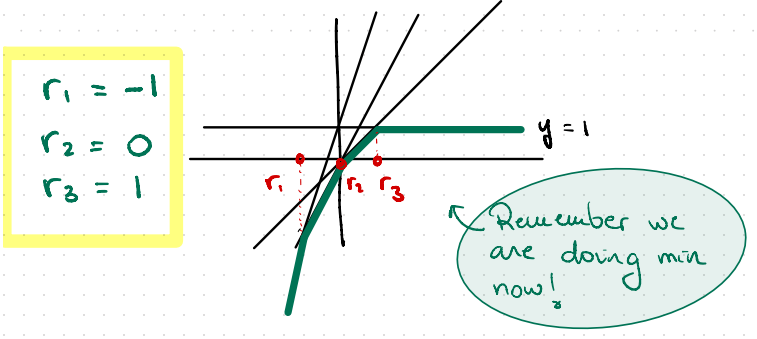
\includegraphics[width=0.85\textwidth]{figs/fig5-1RealizabilityExampleProof.png}
        \caption{Tropicalization of $q$ in $\min$ convention}
        \label{fig:5.1-RealizabilityExampleProof}
    \end{figure}
    The roots of this polynomial are $-1,0$, and $1$. We will now find a root $r_1\in\bC\set{\set{t}}$ of $q$ with $\val(r_1)=r_1$. For this to happen we requiere 
    $$r_1=yt^{-1}+z\word{where}y\in\bC\word{and}z\in\bC\set{\set{t}},\ \val z>r_1.$$
    We now plug in $r_1$ into $q$ and we obtain
    \begin{align*}
        q(r_1)&=t(yt^{-1}+z)^3+(yt^{-1}+z)^2+(yt^{-1}+z)+t\\
        &=\un{y^3t^{-2}}+3y^2zt^{-1}+3yz^2+z^3t+\un{y^2t^{-2}}+2yzt^{-1}+z^2+yt^{-1}+z+t
    \end{align*}
    Extracting the coefficients we get $y^3+y^2=0$ which means that $y=-1$. Plugging this back into our expression as $y$ we get 
    $$3zt^{-1}-3z^2+z^3t-2zt^{-1}+z^2-t^{-1}+z+t=tz^3-2z^2+(t^{-1}+1)z+(-t^{-1}+t).$$
    Tropicalizing (\red{is it actually or is it the reverse operation?}) we get 
    $$1\.z^3+z^2+(-1)z+(-1)$$
    which has as a root $1>-1$ So 
    $$z=y+z_1\word{with}y\in\bC,\quad z_1\in\bC\set{\set{t}}.$$  
    \begin{figure}[h!]
        \centering
        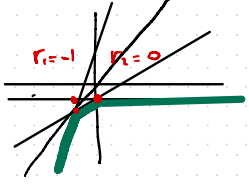
\includegraphics[width=0.5\textwidth]{figs/fig5-2EndOfProofFiniteCase.png}
        \caption{I don't know what this is}
        \label{fig:5.2-EndOfProofFiniteCase}
    \end{figure}
    \red{ASK MAPLE CODE}
\end{Ex} 

The question now is: how do we turn this idea into a formal proof?
\begin{enumerate}[i.]
    \item We do one root at a time, starting with the rightmost one.
    \item Observe that if $r$ is a tropical root and $\al=yt^r$ with $y$ chosen so cancellation happens, then denoting $\tilde{q}$, $q$ without the $x^0$ term:
    $$\Trop(q(x+\al))>\Trop(\tilde{q})\oplus\Trop(q(\al)).$$
    \item Finally we iterate and check that the sequence of $r_i$'s goes to $\infty$.
\end{enumerate}

\subsection{Combinatorialization of Root Finding}

We will be using the $\max$ convention now. So let us consider $p(x)=\sum_{k=0}^da_kx^k$. Can we a systematic and simple way to say how many roots, with what multiplicity, and what equations to solve?\par 
The left-most root can be found via
$$\min\left(\frac{a_0-a_k}{k}\right)=\text{achieved by }k\text{ such that }\frac{a_0-a_k}{k}\text{ is maximized}.$$
In other words we are looking for the largest slope:
\begin{figure}[h!]
    \centering
    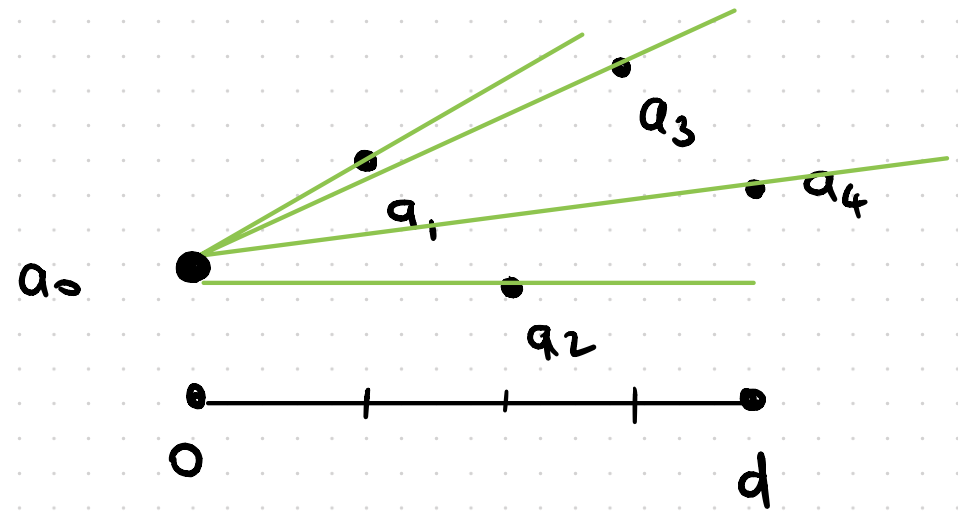
\includegraphics[width=0.5\textwidth]{figs/fig6-1BiggestSlope.png}
    \caption{Difference of coefficients as slopes}
    \label{fig:6.1-BiggestSlope}
\end{figure}
We may repeat this argument for the following roots to get the following algorithm:
\begin{enumerate}[i.]
    \item Let $p_k=(k,a_k)\in\bonj{0,d}\x\set{-\infty}\cup\bR$.
    \item Now $\Sg$ is the convex hull of the points $\set{p_k\:\ k\in[d]}$. We may divide the region into $\Sg^+$ and $\Sg^-$.
    \item Call $q_i=\pi(p_i)$ for $p_i$'s that for the vertices of $\Sg^+$.
\end{enumerate}
The roots will be in bijection with the connected components of $\bonj{0,d}\less\set{q_i}_{i\in I}$ and the multiplicity is the length of the segment.

\begin{Ex}
    Take for example the polynomial 
    $$p(x)=0+1\.x+1\.x^2+x^3+2\.x^4+1\.x^5.$$
    We now place the points in our diagram and project:
    \begin{figure}[h!]
        \centering
        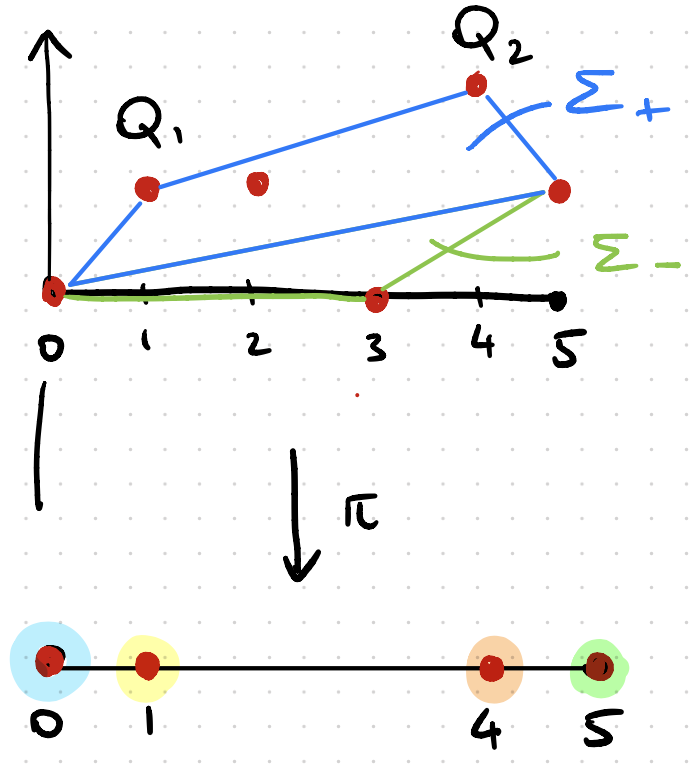
\includegraphics[width=0.5\textwidth]{figs/fig6-2CombinatorializationExample.png}
        \caption{Root finding for $p(x)$}
        \label{fig:6.2-CombinatorializationExample}
    \end{figure}
    From this we deduce that there are $2$ simple roots and $1$ triple root. This come from the equations
    $$
    \left\lbrace
    \begin{aligned}
        &0=x+1&\To x=-1\\
        &x+1=2+4x&\To x=-1/3\\
        &2+4x=1+5x&\To x=1
    \end{aligned}
    \right.
    $$
\end{Ex}

\subsection{Gr\"obner Complexes}

If $K$ is a field with a valuation, then call
$$
\left\lbrace
\begin{aligned}
    &R_K\subseteq K=\text{ elements with non-negative valuation}\\
    &\lie{m}\subseteq R_K=\text{ elements with positive valuation}
\end{aligned}
\right.
$$
so $\quot{R_K}{\lie{m}}$ is a residue field. In the case of tropical polynomials, they form a Gr\"obner complex\footnote{What are Gr\"obner comlpexes? To see in interim.}.
$$\lie{m}=\bigcup_nt^{1/n}\bC\bonj{\bonj{t^{1/n}}}\subseteq R_K=\bigcup_n\bC\bonj{\bonj{t^{1/n}}}\subseteq\bC\set{\set{t}},\word{and}\quot{R_K}{\lie{m}}=\bC.$$

\begin{Def}
    Given $q\in K[x]$ and $w\in\bT$, the \term{initial form} of $q(x)$ with respect to $w$ is a polynomial in $k[x]$that records the part of $q$ that has lowest order when $\val(x)=w$.
\end{Def}

\begin{Ex}
    Let us consider the polynomial 
    $$q(x)=t^{-4}+\sqrt{2}x+3t^2x^2,$$
    Here\footnote{What does this mean?}
    $$t^{-4}\to -4,\quad \sqrt{2}x\to-3,\quad 3t^2x^2\to -4,\word{so}w=-3\footnote{I srsly don't understand}.$$
    We may construct the initial form as $I_wq=1+3x^2$ but formally this is $\bonj{t^4(q(t^{-3}x))}_{t=0}$ and in general if $W=\Trop q(w)$ then 
    $$I_wq=\bonj{t^{-W}(q(t^{w}x))}_{t=0}.$$
\end{Ex}

\subsubsection{Gr\"obner Complex of $q(x)$}

Polyhedral decomposition of $\bR$ (in the case of a valuation space if we want, we can also add in $\infty$ but it usually is left out.) induced by the equivalence relation
$$w_1\sim w_2\iff In_{w_1}q=In_{w_2}q\footnote{Does this refer to initial form?}$$

\begin{Ex}
    Consider the polynomial 
    $$t^2+\sqrt2x+3t^2x^2$$
    and each monomial maps\footnote{Through what? The valuation?} to $2,w$ and $2+2w$ respectively.
    \begin{figure}[h!]
        \centering
        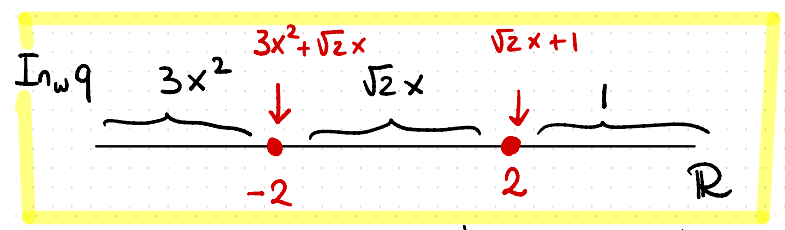
\includegraphics[width=0.5\textwidth]{figs/fig6-3-InitialFormExample.png}
        \caption{Initial form determination and roots}
        \label{fig:6.3-InitialFormExample}
    \end{figure}
    So the tropical roots are the locus where the initial form is not a monomial.
\end{Ex}
\section{Day 7|20230906}

\subsection{Our First Correspondence Theorem}

\begin{Def}
    Given a family of polynomials 
    $$q_t=\sum A_k(t)x^k\in\bC[x]\word{with}t>1$$
    then the \term{tropicalization} of $q_t$ is 
    $$\Trop(q_t)(x)=\sum a_k\odot x^{\odot k},\word{where}a_k=\lim_{t\to\infty}T_t(A_k).$$
    We may also use the $\min$ convention by exchanging the field to Puiseux series and $T_t$ by the valuation.
\end{Def}

\begin{Th}[Correspondence]
For a polynomial $q_t$, $R_t$ is a root of $q_t$ if and only if $\Trop(R_t)=\lim_{t\to\infty}T_t(R_t)$ is a root of $\Trop(q_t)$.
\end{Th}

This is saying that we have an object in algebraic geometry, a polynomial. Tropical geometry will somehow knowing about its roots by degenerating it. Then its easy to find the tropical roots and then there must be certain algebraic roots which should map to them. It may not be easy to understand this last map but at least we have some qualitative information.\par 
We will use the fundamental theorem of algebra to reduce to the linear case. So the first step is to prove the theorem for the case of linear polynomials. We have a couple of lemmas to finish the proof and expand it to the general case:

\begin{Lem}
    $\Trop$ is a multiplicative function on polynomials. That is
    $$\Trop(pq)=\Trop(p)\odot\Trop(q)\word{for}p,q\in\bC[x].$$
    \end{Lem}
    
This first lemma doesn't add anything weird because the tropical product is just the usual addition.

    \begin{Lem}
    The roots of $\Trop(p)\odot\Trop(q)$ are the union of the roots of the factors. If a root is repeated then the multiplicities are added.
    \end{Lem}

    Essentially what this is saying is that if we have two piecewise linear functions which change slope at the same place, then the sum will also change slope at the same place. As the functions are convex, a root can never be cancelled. Except possibly $-\infty$.

    \subsection{Higher Dimension}

    We will go back to the Puiseux series convention now:
    $$P(X)\in\bC\set{\set{t}}\bonj{X},\ P(R)=0\iff \Trop(P)(\val(R))=0.$$
    The easy direction is to begin with a root of our Puiseux polynomial. Let 
    $$P(X)=\sum A_i(t)X^i,\word{and}\Trop(P)(X)\sum a_i\odot x^i$$
    where $a_i=\val(A_i)$. Let $R=R(t)$ be a root of $P(X)$.\par 
    We know $\val(P(R))=\infty$ because $P(R)=0$. Formally $\val(P(R))$ should greater or equal than the minimum of the valuation of each of the monomials evaluated at $R$. In other words 
    $$\min(\val(A_i(t)R^i))=\min_i(a_i+i\val(R))=Trop(P)(R).$$
    Since we know that strict inequality holds, the terms in the formal evaluation with lowest order must cancel, in other words, the minimum is attained at least twice by two different monomials.\par 
    Last week we mentioned attaining the minimum twice is the same as being a root.

    \begin{Ex}
        Consider the polynomial $(t^2+7t^3)X+(t^5+t^{27})=Q(X)$. The root here is $R=-\frac{t^5+t^{27}}{t^2+7t^3}$ and its valuation is $5-2=3$. If we plug in something of this form instead of $X$ we get 
        $$Q(-t^3+O(t^4))=(t^2+7t^3)(-t^3+O(t^4))+(t^5+t^{27})=(-t^5)+t^5+O(t^6)$$
        In particular the first thing that will cancel is the lowest order term: $t^5$. So \emph{two} monomials must have lower order term.
    \end{Ex}

\section{Day 10|20230913}

The next question is if this process makes sense if we instead begin with a Puiseux series polynomial. If the process ends up being the same, does this mean that tropical geometry over a trivial valued field is uninteresting? That's not the case, it's only because we are in dimension zero. 

\subsection{Gr\"obner Complexes}

These types of complexes arise in commutative algebra. The setup begins with a valuated field, in our case Puiseux series $\bC\set{\set{t}}$. We can find the ring of integers, the positive valuated elements, in our field. These types of functions are regular at $t=0$. Inside this ring we have the maximal ideal of functions which vanish at zero. If we wish we can take a quotient to find the residue field which is a copy of $\bC$.\par 
Everytime we are given the data of polynomial $q$ in $\bC\set{\set{t}}\bonj{x}$ plus a choice of a valuation, we can recover the initial form of $q$ which is a polynomial with coefficients in the residue field.\par 
The way to find it is to look at the valuation of each monomial assuming $\val(x)=w$ and then save only the monomials with the smallest valuation and only keep the coefficient in front of the smallest term.

\begin{Ex}
    Consider the polynomial 
    $$q(x)=t^{-4}+t^{2}+\sqrt{2}x+3t^2x^2$$
    and take $w=-3$. This means that $\val(x)=-3$. Let us now consider the valuation monomial by monomial:\par 
    The term $(t^{-4}+t^{2})$ has valuation $-4$ because there's no $x$, next for $\sqrt{2}x$ we have
    $$\val(\sqrt{2}x)=\val(\sqrt{2})+\val(x)=0+(-3)=-3$$
    so it has valuation $-3$ and $3t^2x^2$ has valuation $2-6=-4$. We now consider only the first and last terms as they have the smallest valuation and extract the coefficients of the smallest terms. In the case of $t^{-4}+t^{2}$ its the $1$ accompanying the $t^{-4}$ and a $3$ accompanying the last term. So the initial form is 
    $$\operatorname{In}_{-3}(q)=1+3x^2.$$
\end{Ex}

\red{FORMULA for initial form}\par 
We now define an equivalence relation over $(\bR,w)$: 
$$w_1\sim w_2\iff In_{w_1}q=In_{w_2}q$$ 
which separates $\bR$ into two types of equivalence classes:
\begin{itemize}
    \item Single points in which the initial form is not a monomial.
    \item Open intervals where the initial is a monomial.
\end{itemize}

\begin{Ex}
    Consider the polynomial 
    $$t^2+\sqrt2x+3t^2x^2$$
    and each monomial maps\footnote{Through what? The valuation?} to $2,w$ and $2+2w$ respectively.
    \begin{figure}[h!]
        \centering
        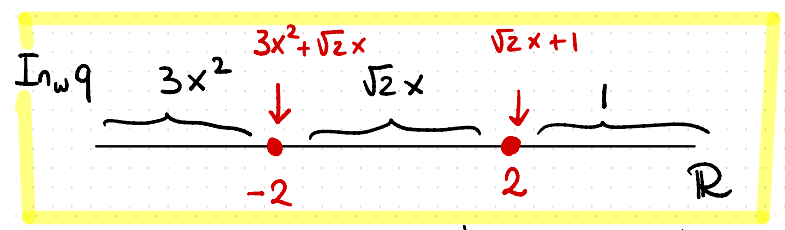
\includegraphics[width=0.5\textwidth]{figs/fig6-3-InitialFormExample.png}
        \caption{Initial form determination and roots}
        \label{fig:6.3-InitialFormExample}
    \end{figure}
    So the tropical roots are the locus where the initial form is not a monomial.
\end{Ex}

\begin{Def}
    The complement of the locus where the initial form is a monomial is called the \term{Gr\"obner complex} of $q(x)$.
\end{Def}

The Gr\"obner complex of $q(x)$ is equal to the roots of $\Trop(q)(x)$. This is indeed in correspondence with Gr\"obner basis, which is very interesting in higher dimension. 

\subsection{1-dimensional Tropical Geometry}

If we have $p(x,y)$ a tropical polynomial in two variables, then we can define its tropical variety to be $V(p)$:
\begin{itemize}
    \item The locus in the domain where the piecewise linear function where $p$ is not linear.
    \item The locus of points $(x,y)$ where the $\max$ associated to each monomial is obtained more than once.
\end{itemize}

We will have a correspondence theorem which says that if $q(x,y)$ is a polynomial with coefficients over a valued field and the tropicalization of $q$ is $p$, then 
$$V(p)=\ov{\set{(\val(x),\val(y))\: (x,y)\in V(q)}}.$$
\begin{Ej}
Show that pairs of rational numbers are dense here. \aside{It has to do with the valuation only taking rational numbers.}
\end{Ej}
In two dimensions we have way more features, the study of tropical curves will enclose the correspondence statement with subdivisions of Newton Polygon and balancing edge weights. Our objective now is to see the tropical versions of tropical curve theorems. For example, the tropical Bézout and tropical degree/genus formula.

\section{Day 11|20230915}

\subsection{Tropical Lines}

\subsubsection{The $\max$ convention}

If we have a tropical polynomial of degree 1, 
$$p(x,y)=a\odot x\oplus b\odot y\oplus c$$
and assume for the sake of drawing pictures, that $-\infty\neq a,b,c$. This corresponds to the piecewise linear function 
$$\max(a+x,b+y,c)$$
and if we set any of these two equations equal to each other, we can see that there are three lines that play a role:
\begin{align*}
    &a+x=b+y\To y=x+(a-b)\\
    &a+x=c\To x=c-a\\
    &b+y=c\To y=c-b
\end{align*}
So this is the locus where two functions are equal to each other. In each of the regions the maximum is attained by a particular linear function, the boundary between them is the locus of non-linearity. The point in the middle is $(c-a,c-b)$. 

\begin{figure}[h!]
    \centering
    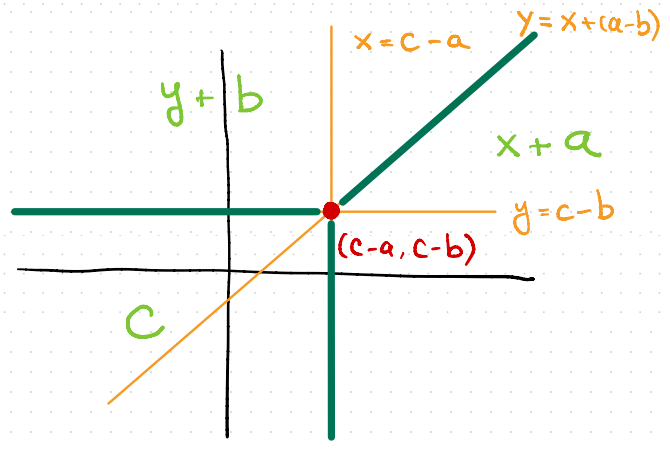
\includegraphics[width=0.5\textwidth]{figs/fig7-1-TropicalLineExample.png}
    \caption{Graph of $p(x,y)=0$ in $\bR^2$}
    \label{fig:7.1-TropicalLineExample}
\end{figure}

So in general, tropical lines look like this ``tripod'' and changing the $a,b,c$ shifts the graph. 

\begin{Ej}[2]
Figure out what happens when a coefficient is $-\infty$.
\end{Ej}

This is analogous to what we have done with tropical univariate polynomials. The tropical line $V(p)$ is the locus of non-linearity of our function:
$$V(p)=\set{(x,y)\in\bR^2\:\ df_p\!\mid\!_{(x,y)}\text{ isn't defined}}.$$
\subsubsection{The Case of Puiseux Series}

In this case, lines will we the zero loci of polynomials of the form 
$$p(X,Y)=A(t)X+B(t)Y+C(t)$$
with 
$$a=\val(A),\quad b=\val(B)\word{and}c=\val(C).$$
We let $L=\set{(X,Y)\in\bK^2\:\ p(X,Y)=0}$ be the zero locus and then define
$$\Trop(L)=\ov{\set{(\val(X),\val(Y))\:\ (X,Y)\in L}}\subseteq\bT^2.$$
We may parametrize $p$ in the following way, we let $X=\ga(t)$ with an arbitrary valuation and then we solve for $Y$:
$$Y=\underbrace{\frac{-A(t)}{B(t)}\ga(t)}_{a-b+\val\ga}-\underbrace{\frac{C(t)}{B(t)}}_{c-b}$$ 
\red{ASK RENZO} Depending on the value of $\val\ga(t)$, then we may get different values for $\val Y(\ga(t))$. 
\begin{itemize}
    \itemsep=-0.4em 
    \item If $\val\ga(t)>c-a$, then $\val Y(\ga(t))=c-b$.
    \item If $\val\ga(t)<c-a$, then $\val Y(\ga(t))=x+a-b$.
    \item And if $\val\ga(t)=c-a$ then $\val Y(\ga(t))$ can be anything above $c-b$. We thus set 
    $$\ga(t)=\left(-\frac{C(t)}{A(t)}\right)(1+t^{\odot m}),\word{where}m>0$$
\end{itemize}
The first two items represent a graph of $(a-b)x+(c-a)$\footnote{ask Renzo because I don't understand, page 4 of TG7.}
\begin{Rmk}
If we send $a,b,c,X$ and $Y$ to their negatives then $\Trop(L)$ agrees with the previous perspective. Alternatively, we can check that $\Trop(L)$ agrees with the previous perspective but using the $\min$ convention.
\end{Rmk}
\begin{Ex}
    Let us explicitly choose $A,B$ and $C$:
    $$q(X,Y)=t^aX+t^bY+t^c.$$
    Note that $q$'s tropicalization is $p(X,Y)$.
    Points in $V(q)$ can be parametrized as 
    $$X=\al,\quad Y=\frac{-t^a}{t^b}\al-\frac{t^c}{t^b}=-t^{a-b}\al-t^{c-b},\word{where}\al\in\bK^\ast.$$
    Taking valuations of $X$ and $Y$ we get $\Trop(L)$ (but without closing it). Specifically we are looking at the set 
    $$\Trop(L)=\set{\left(\val(\al),\val(-t^{a-b}\al-t^{c-b})\right)\in\bT^2\:\ \al\in\bK^\ast}$$
    We can let $\al$ have any valuation we want and depending on that, we determine the valuation of the binomial $Y$. The possible valuations are 
    $$\val Y=a-b+\val(\al)\word{or}\val Y =c-b$$
    which are equal when $\val(\al)=c-a$. \red{ASK RENZO ABOUT THIS HOW TO DETERMINE THE CRITERION ABOUT VAL AND STUFF}
    \begin{itemize}
        \item What happens if $\val(\al)<c-a$ then $-t^{a-b}$
        \item Something I fell asleep 
    \end{itemize}
    \textbf{Claim: We can obtain any value for $y$ but is to be greater than $c-b$.}
    Let $r\geq 0$ and $\al=-t^{c-a}(1+t^r)$
\end{Ex}

\begin{figure}[h!]
    \centering
    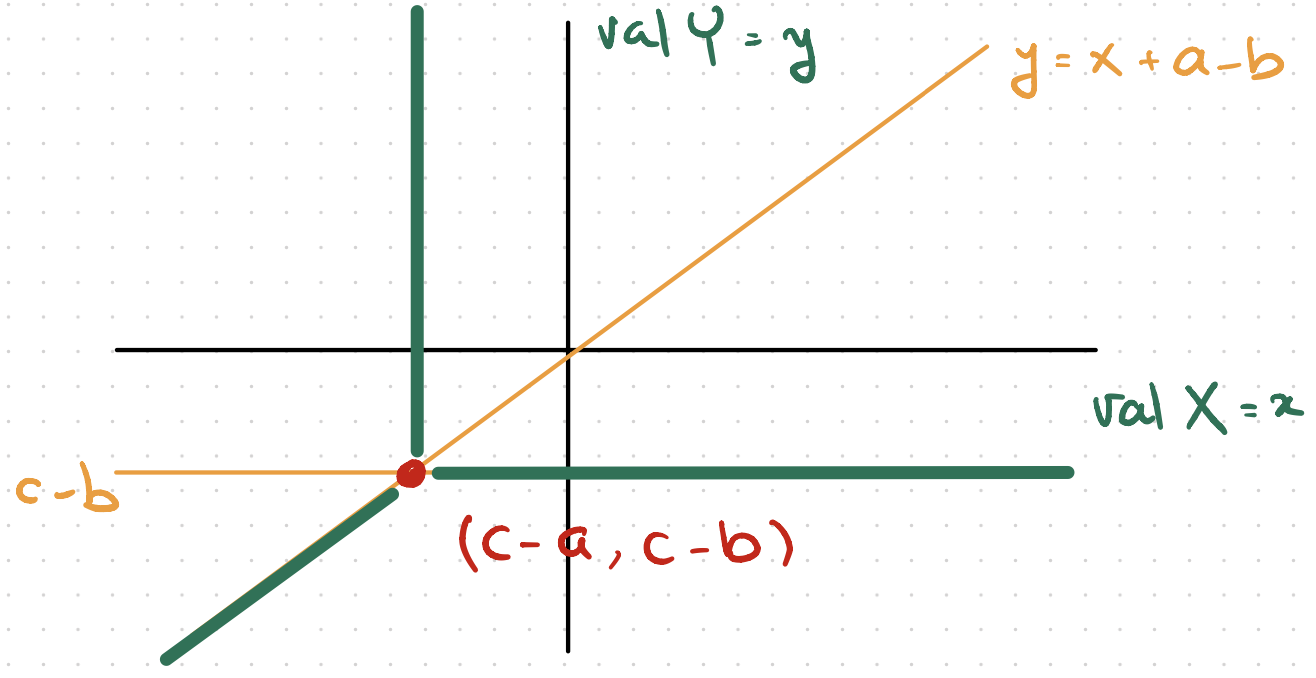
\includegraphics[width=0.5\textwidth]{figs/fig7-2-TropicalLinePuiseuxExample.png}
    \caption{The tropical line from the Puiseux perspective}
    \label{fig:7.2-TropicalLinePuiseuxExample}
\end{figure}

\subsubsection{Glimpse into Amoebas}

Recall that what matters the most is the logarithm base $t$ of our function. So let us continue with 
$$q(x,y)=t^ax+t^by+t^c$$
and play the same as before. Look for solutions to the equation $q_t=0$ in $\bC^2$ which is a line intersecting the $x$ axis at $-t^{c-a}$ and the $y$ at $-t^{c-b}$. Every pair of points $(x,y)$, gives us a pair $(\log_t|x|,\log_t|y|)$. The real trace of this, when $x,y\in\bR$ can be parametrized with $x=t^\al$ and $y=-t^{a-b+\al}$. We analyze the trace in three intervals, 

\section{Day 12|20230918}

\subsection{The Amoeba Perspective}%%VAMOS POR AQUI TG7

Our goal is to understand the image of the line 
$$L_t=\set{t^ax+t^by-t^c=0}\subseteq\bC^2$$
via the map $(x,y)\mapsto (\log_t|x|,\log_t|y|)$. The line $L_t$ has three sections, where both $x,y$ are positive and one section corresponding to each $x$ and $y$ being negative. For ease of calculation we may solve the equation as $y=-t^{a-b}x+t^{c-b}$\par 
Let us consider the case where $x,y$ are both positive. We can see that $0<x<t^{c-a}$, this traces an $x$ in the parameter space such that $-\infty<x<c-a$. Via the solution for $y$ we may write 
$$\log_t|y|=\log_t(t^{c-b}-t^{a-b+x})$$
where we have solved the equation for $x$ which is why we have an $x$ exponent and $y$ is positive as we have assumed. We can simplify this as 
$$\log_t\bonj{t^{c-b}\left(1-t^{a-c+x}\right)}=(c-b)+\log_t(1-t^{a-c+x}).$$
This can be traced as a function of $t$ and in particular
$$\lim_{x\to-\infty}(c-b)+\log_t(1-t^{a-c+x})=c-b\word{and}\lim_{x\to(c-a)^{-}}(c-b)+\log_t(1-t^{a-c+x})=-\infty.$$
With this information we see two asymptotes for our function, $y=c-b$ and $x=c-a$.

\subsection{Arbitrary Degree $d$}

Recall that for a polynomial $q\in\bK[x,y]$, we may describe its algebraic variety in $\bK^2$. We may think of that field as Puiseux series. Along it, we may tropicalize it to $p$ and we get its tropical hypersurface, the set of non-linearity.\par
Kapranov's theorem allows us to see a correspondence as follows:
$$\ov{\Trop(V(q))}=V(\Trop(q)).$$
Left-to-right is still the same idea as the correspondence theorem. If $(x_0,y_0)\in\Trop(V(q))$ then, there exists $(X_0,Y_0)\in\bK^2$ such that $\val(X_0)=x_0,\ \val(Y_0)=y_0$ and $q(X_0,Y_0)=0$. Let 
$$q=\sum a_{ij}X^iY^j$$
If we call $m_{ij}$ each monomial, then $\set{m_{ij}(X_0,Y_0)}_{i,j}$ is a set of elements of $\bK^\ast$ with the property that their sum is zero. Now call 
$$\mu=\min\set{m_{ij}(X_0,Y_0)}_{i,j}$$
we claim that there are at least two monomials whose valuation is $\mu$. If there was only one monomial with valuation $\mu$, then that power of $\mu$ \emph{cannot} be cancelled. This means that $(x_0,y_0) $ is in $V(p)$. Now we use minimality of closure and we are done.\par 
Now the harder direction will use the fact that we have proven this in dimension zero and proceed by induction. First we want to show that $V(\Trop(q))\cap\bQ^2$ is dense in $V(\Trop(q))$. This is true because all monomials $m_{ij}$ correspond to all linear functions with integer slopes of rational coefficients.
$$a_{ij}X^iY^j=\Trop(m_{ij})=\val(a_{ij}\odot x^{i}\odot y^j)=\val(a_{ij})+ix+jy$$
It suffices to check that \red{ERASED TOO QUICK}\par 
Now we wish to proceed by induction. For example a polynomial $q(X,Y)$ can be seen as 
$$q(X,Y)=r_0(X)+r_1(X)Y+\dots+r_d(X)Y^d\word{with}r_i(X)\in\bK[X].$$
We do not lose generality when assuming that all $r_i$'s are monomials\footnote{to see next time}. So we have $(x_0,y_0)\in\in V(\Trop(q))$ and we want to find $(X_0,Y_0)\in(\bK^\ast)^2$ such that 
$$q(X_0,Y_0)=0\word{and}(\val(X_0),\val(Y_0))=(x_0,y_0).$$
Choose $X_0$, however we want as long as we have the valuation condition. Given our assumption, this implies that $r_i(X_0)$ is non-zero for all $i$. Now consider the polynomial 
$$q(X_0,Y)=\sum r_i(X_0)Y^i\in\bK[Y]$$
and its tropicalization
$\tilde{p}(y)=\Trop(q(X_0,Y))=\sum\val(r_i(X_0))y^i=\min(\val R_i(X_0)+iy)=\min$
They are hidden in terms of unknown,

\section{Day 13|20230920}

\begin{Th}
$V(\Trop(q))=\ov{\Trop(V(q))}$
\end{Th}

If we start with a polynomial in valued field, we can tropicalize or look at ... and then take the image of coordinates of points and back in $\bR^2$ then take closure, we end in the same place. The fact that every point of the algebraic curve  lies somewhere is an argument of cancellation of Lowest Order Terms. In particular when plugging the value for the Puiseux solution two terms must cancel. 
\begin{ptcbp}
We have shown that right-to-left is easy, cancellation of L.O.T.\par 
The other direction is trickier, it's a lifting problem. Given $(x_0,y_0)\in V(\Trop(q))\subseteq\bR^2$, then we must find 
$$(X_0,Y_0)\in V(q)\subseteq \bK^{\ast2},\quad\val(X_0)=x_0\quad\val(Y_0)=y_0$$
If we write $q$ then we will assume that we can write 
$$q(X,Y)=\sum r_i(X)Y^i,\quad r_i(X)\ \text{monomials}$$
If we first plug in $X=X_0$ (which is any Puiseux series we want with valuation $x_0$ [We have picked such $X_0$]), 
$$q(X_0,Y)=\sum r_i(X_0)Y^i$$
is a polynomial in $Y$ with Puiseux series coefficients, now tropicalize this $q$ we get 
$$\tilde{p}(y)=\sum\val r_i(X_0)y^i\quad\text{(tropical sum and product now)}.$$
We claim that $y_0$ is a root of $\tilde{p}(y)$. HEre's where we are using the monomial assumption.\par 
What is the linear function associated to $\tilde{p}(y)$:
$$\tilde{p}(y)=\min(\val r_i(X_0)+iy)$$
and as $r_i$ is monomial, call it $r_i(X_0)=A_{ij}X^j$ where $A_{ij}$ is a Puiseux series. So this $\tilde{p}$ becomes:
$$\tilde{p}(y)=\min(\val(A_{ij})+jx_0+iy)$$
which is exactly the tropicalization of $q(x,y)$ and plug in $x_0$. This is a univariate polynomial, which allows to apply the univariate case. So there exists a $Y_0$, Puiseux series, such that $Y_0$ is a root of $q(X_0,Y)$ with $\val(Y_0)=y_0$.\par 
It remains to see that our monomial condition is not a restriction. 
\end{ptcbp}

This allows us not only to lift, but to pick one coordinate freely and then the other one is determined!

\begin{Ex}
    Consider the polynomial 
    $$q(X,Y)=XY+X^2Y=(X+X^2)Y,\word{and}\tilde{q}(X,Y)=q(XY,Y)=XY^2+X^2Y^3$$
    and $\tilde{q}$ does satisfy the previous assumption. If $(\tilde{X}_0,\tilde Y_0)$ is a solution to our problem for $\tilde{q}=0$, then $\left(\frac{\tilde{X}_0}{\tilde Y_0},\tilde Y_0\right)$ is a solution for $q=0$.\par 
    The key point is that $\tilde q$ is obtained $q$ by an invertible transformation in the torus $(\bK^\ast)^2$.
\end{Ex}

\begin{ptcb}
Given $q(X,Y)$ of degree $d$, then picking 
$$\tilde{q}(X,Y)=q(XY,Y^{d+1})$$
satisfies the monomials assumption. This is because \emph{we are giving enough space}.
$$q(X,Y)=\sum r_{ij}X^iY^j\To \tilde{q}(X,Y)=\sum r_{ij}X^iY^{(d+1)j+i}$$
where if we wished to find \dots then 
$$(d+1)j_1+i_1=(d+1)j_2+i_2\To (d+1)(j_1-j_2)=i_2-i_1$$
$j_1-j_2\geq d+1$ when $j_1=j_2$ and $i_2-i_1\leq d$.
\end{ptcb}

\begin{Ex}
    Compute $V(p)$ for the following polynomials
    \begin{itemize}
        \item $p_1=0+x+y+xy$
        \item $p_2=0+x+y-xy$
        \item $p_3=0-x-y+xy$
    \end{itemize}
    For each of this polynomials there are $\binom{4}{2}=6$ line possibilities so we check each one.
\end{Ex}

\section{Day 14|20230922}

Consider the polynomial 
$$q(X,Y)=XY+X+Y+c,\quad c\in\bC$$
as a polynomial in $\bK[X,Y]$ such that $\Trop q=p$. We can factor $q$ as 
$$(X+1)(Y+1)+(c-1)=0\To(X+1)(Y+1)=\tilde{c}$$
which looks hyperbolic. The real locus is PICTURE and we would like to compactify. However in $\bP^2$ we get an anomalous curve. PICTURE So we would like to compactify instead in $\bP^1\x\bP^1$.  We bi-homogenize $q$ to obtain 
$$\tilde{q}=X_1Y_1+X_1Y_0+Y_1X_0+X_0Y_0c=0$$ 
In this case PICTURE we won't intersect the special points. Instead just general points. The point we want to emphazise is the fact that the shape of the tropical curve tells us that this could be the tropicalization of  a curve but that the plane curve wants to be compactified in $\bP^1\x\bP^1$ instead of $\bP^2$.

\subsection{Bummer Theorem}

\begin{Th} 
    Let $q\in\bC[X,Y]$ considered as a subset of Puiseux series polynomials where no coefficient is zero. We can write $q(X,Y)=\sum_{i+j\leq d}a_{ij}X^iY^j$ with $a_{ij}\neq 0$.\par 
    Then $\ov{\Trop(V(q))}$ looks like a tropical line with a vertex at zero.
\end{Th}

This is a bummer because any polynomial of this form will look like a tripod. But what happens with \emph{lines off to infinity matches the degree}? We may able to endow lines with information about the degree, but nonetheless, we lose every other piece of information. So choosing coefficients in a trivially valued field reduces all information.\par 
To prove this theorem we will unravel the definitions.

\begin{ptcbp}
We have that the tropicalization of $q$ is 
$$\Trop q=\bigoplus(x^i\odot y^j)=\min_{i+j\leq d}(ix+jy)$$
and so we can see that the minimum is attained by PICTURES
\end{ptcbp}

Working with Puiseux series is not only because its fancy, its because we wish to have non-trivial objects.

\subsection{Structure Theorem for Tropical Curves}

Let $p(x,y)=\bigoplus a_{ij}\odot x^i\odot y^j$ be a tropical polynomial. The Newton polygon of $p$ is the convex hull of $(i,j)$ such that $a_{ij}\neq 0$.\par 
Let $\Sg$ be the convex hull of the points $(i,j,a_{ij})\subseteq V(NP)\x\bR$, which is for every $(i,j)$ point consider the height $a_{ij}$ so $\Sg$ is a convex polytope in $\bR^2\x\bR$. Seeing the polytope from the top and projecting down we get a subdivision of the Newton polygon.\par 
Consider $\pi_z((x,y),z)=(x,y)$ and let $\tilde{N}$\~N be the subdivision of the N.P. obtained by projecting the corners of $\Sg$ you can see from above.
If we want to say this in fancier words, a polytope is a finite intersection of half-spaces and then we look at intersections of planes with outward normal vector ($z$ postive coordinate) then project down to $xy$ plane.\par 
Then the tropical curve is \textbf{DUAL} to such subdivision, meaning that:
\begin{itemize}
    \item Vertices of the tropical curve map to faces of \~N, edges map to edges of \~N.
    \item There is a reversing structure given by inclusion into the closure.
    \item Every edge of $V(p)$ is perpendicular to the edges of \~N, it corresponds to.
    \item Coordinates of vertices $v$ are found by solving the linear system obtained by setting equal the linear functions corresponding to monomials corresponding to vertices of the face of \~N dual to $v$.
\end{itemize}

\begin{Ex}
    Consider the polynomial
    $$p(x,y)=0\oplus x^2\oplus y^2\oplus 1x\oplus 1y\oplus xy,$$
    each monomial corresponds to a vertex in our triangle. Somehow now we know that our tropical curve has 4 vertices, then we can correspond edges.\par 
    To get the coordinates of the lowe left vertex we look at the vertices surrounding the corresponding triangle. The linear system we ought to solve is 
    $$0=1+x=1+y\To x=-1,\ y=-1$$
    and in this fashion we obtained the coordinates. 
\end{Ex}

\section{Day 15|20230925}

We were talking about how tropical plane curves are dual to the subdivisions of the Newton polygon of the tropical polynomial. Let's recall this with an example. 

\begin{Ex}
    Consider the polynomial $0+x^2+y^2+x+y+xy$. All coefficients are non infinity so we get 6 points corresponding to all terms, the convex hull is a triangle. We give each point a height, $0,x^2$ and $y^2$ have $0$ coefficient while $x,y$ and $xy$ have coefficient $1$. We imagine throwing a drape over that figure and then divide the faces, edges of tropical curve are perpendicular so the curve should look similar to the following figure.\par
    \red{FIGURE}\par 
    Now for example, the central vertex is dual to the face $F_2$ which corresponds to the monomials $1+x$, $1+y$ and $1+x+y$. The solution to the system 
    $$
    \left\lbrace
    \begin{aligned}
        &1+x=0\\
        &1+y=0\\
        &1+x+y=0\\
    \end{aligned}
    \right.
    \To (x,y)=(0,0)
    $$
    so $(0,0)$ is the coordinate of the central vertex.
\end{Ex}

\begin{Rmk}
There's not metric duality between the triangle and the curve! It is possible to make a Newton polygon which doesn't fit in the curve as well.
\end{Rmk}

\begin{Ej}[5]
Find such an example!
\end{Ej}

If we did this in the case of Puiseux series, then the subdivision of the Newton polytope keeps track of the initial forms of $q$ in the sense that for any cell in the Newton subdivision, the initial form is given by the monomials corresponding to the lattice points in this set.

\begin{Ex}
    Consider the polynomial 
    $$q(X,Y)=7+3X^2+2Y^2+t^{-1}X+2t^{-1}Y+t^{-1}XY,$$
    this polynomial tropicalizes via $-\val$ to the polynomial $p$ from last example.\par \red{FIGURE}\par 
    The initial form in the face $F_1$ corresponds to the monomials $XY+2Y+2Y^2$, then $XY+2Y+X$ in $F_2$, $X+2Y+7$ in $F_3$ and $3X^2+X+XY$ in the last $F_4$. The Gr\"obner fan is still the same as in the tropical curve.\par 
    Along the edge $01$ of $F_1$ the initial form is $2Y^2+XY=In_w(q)$ where $w=(w_1,w_2)=-(\val X,\val Y)$ for $w$ in the blue edge of the tropical curve (corresponds to \red{stuff} which has that initial form). 
\end{Ex}

We will prove this fact by making a crucial observation. Evaluating a tropical monomial at a point $(x_0,y_0)$ can be done as a dot product. Take $m=a\odot x^i\odot y^j$ so the evaluation is at $(x_0,y_0)$ is 
$$\braket{(i,j,a)}{(x_0,y_0,1)}.$$
When we construct the subdivision of the N.P. we consider all points with coordinates $(i,j,a_{ij})$ as $i,j$ ranges over $\set{a_{ij}\neq -\infty}$
So evaluating $p(x_0,y_0)$ amounts to looking for the maximum of the dot products of $(x_0,y_0,1)$ with all $(i,j,a_{ij})$.\par 
\red{FIGURE}\par 
In other words $m_{ij}(n_x,n_y)$ is equal for all monomials corresponding to vertices of the green face. For vertices below, it occurs that $\braket{\vec n}{\vec v}<0$ so 
$$m_{ij}(n_x,n_y)<m_{\tilde i\tilde j}(n_x,n_y)$$
when $m_{ij}$ corresponds to vertices not in the face and $m_{\tilde i\tilde j}(\dots)$ in face.\par 
We have identified why the vertices correspond to tropical subdivisions, but the edges? If we focus on one, it bounds two faces $F_1$ and $F_2$ which span two planes with normal vectors $\vec n_1,\vec n_2$ with their respective $z$ coordinates equal to $1$. So any vector between these two, i.e. any one in with first two coordinates in the segment $n_1$ to $n_2$ has the property that 
$$\braket{n}{m_1}=\braket{n}{m_2}>\braket{n}{m_{\text{other}}}$$ %Nate tiene los dibujos y revisar notas en canvas

\section{Day 16|20230927}

We have discussed that tropical plane curves are dual to a subdivision of the Newton polytope. There's a combinatorial algorithm that will allow us to divide the N.P.\par 
We will study a couple more characteristics to discern between stick figures and tropical curves. We need to introduce the fact that each \emph{stick} gets a weight.

\begin{Def}
    Any edge of a tropical curve $V(p)$ is given \term{weight} $w_e$ equal to the lattice length of the segment of the N.P. subdivision dual to the edge.
\end{Def}

Before even defining what things mean, let see an example. 

\begin{Ex}
    Consider the tropical cubic with subdivision edges $1\to yx^2$ and $yx^2\to y^2$. We may identify weights of edges with black in the coming figure:
    \begin{figure}[h!]
        \centering
        %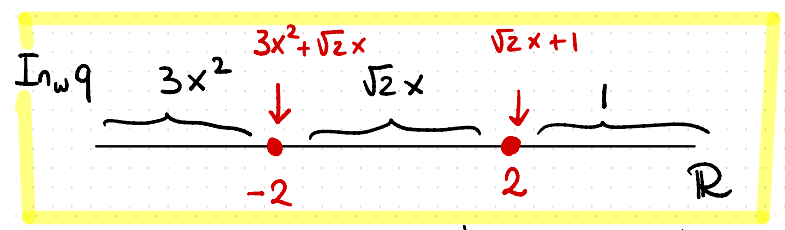
\includegraphics[width=0.5\textwidth]{figs/fig6-3-InitialFormExample.png}
        %\caption{Initial form determination and roots}
        %\label{fig:6.3-InitialFormExample}
    \end{figure}
\end{Ex}

\begin{Th}
Tropical plane curves are balanced, meaning that at every vertex
$$\sum_{v\in e}w_e\vec p_e=0.$$
Here $w_e$ is the weight of the edge $\vec p_e$ outgoing primitive vector in the direction of $e$.
\end{Th}

Continuing the line of the previous example, at the vertex we were looking at we have outgoing primitive vectors 
$$\twobyone{1}{2},\quad\twobyone{-1}{0}\word{and}\twobyone{1}{-2}.$$
Observe that when taking the weighted sum at the vertex we get 
$$2\twobyone{-1}{0}+\twobyone{1}{2}+\twobyone{1}{-2}=\twobyone{0}{0}.$$
We will prove the theorem next.

\begin{ptcbp}
Any vertex is dual to a face $F_v$ of N.P. subdivision.
For every edge bounding $F_v$, the vector $w_e\vec p_e$ is obtained by the vector tracing the dual edge via a $90^circ$ rotation. We claim to be done, the fact that the equation is satisfied is equivalent to the fact that the N.P. is a closed polygon.
\end{ptcbp}

So imagine a stick figure with weighted edges comes up to you, then we can check the compatibility condition. If it doesn't have weights, does there exist an assignment of weights in order to form a tropical curve? 

\subsection{What do the weights mean?}

\begin{Ex}
    Suppose we have a subdivision with edges 
    $$x^2y\to x^5y^2\to x^8y^3\to x^11y^4$$
    and the corresponding edge in the tropical curve. We want to see the initial form. This subdivision \emph{remembers} the monomials that appear in the initial form! It will be a linear combination of the monomials in the edge!
    $$\operatorname{In}_\omega(q)=Ax^2y+Bx^5y^2+Cx^8y^3+Dx^{11}y^4=x^2y(A+Bx^3y+Cx^6y^2+Dx^9y^3)=x^2yP(x^3y)$$
    This polynomial factors so nicely because they lie on the same line! If we are just looking for solutions in $(\bC^\ast)^2$ or asymptotically $|x|,|y|\gg 0$ what happens is that the monomial part is irrelevant. Also $\deg(P)$ is equal to the lattice length of the segment. A 1-parameter subgroup orbits $x^3y=r_i$ where the $r_i$ is a root of $P$ counted with multiplicity.    
\end{Ex}

\section{Day 17|20230929}

Last time we talked about edges weighted by lattice length determines the segments of the Newton Polygon it is dual to. Today we will draw topological types of tropical plane curves and cubics. The objective is to experiment with various tropical curves and seek a conjecture to compute their $b_1$. Study a pencil of tropical conics, in other words draw a conic and pick 4 points on it in general position. Then find all conics through those 4 points.

\section{Day 18|20231002}%% TG11

For any interior point of the Newton Polygon, we can make sure that we can find as many cycles can a tropical curve have. There is a correspondence theorem.\par 
The solution to the parameter space of conics is that we get a trivalent tree with $6$ edges. This corresponds to $\bP^5$ which has $6$ boundary divisors.

\subsection{Intersections of tropical curves}

\begin{Def}
    Two tropical curves have a \term{transversal intersection} if they intersect in finitely many points which are not vertices of either curve.
\end{Def}

\begin{Ex}
    Two tropical lines seen as tripods which touch just at a point intersect transversally. 
    \begin{figure}[h!]
        \centering
        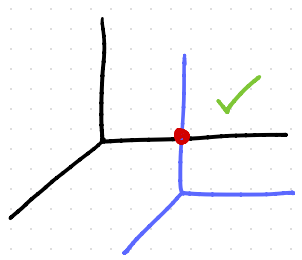
\includegraphics[width=0.5\textwidth]{figs/fig11-1-TransversalIntersectionExample.png}
        \caption{Example of a Transversal Intersection}
        \label{fig:11.1-TransversalIntersectionExample}
    \end{figure}
\end{Ex}

\begin{Ex}
    If the line is placed right on top of the other one, they could also intersect non-transversally on the whole edge.\par 
    If for example we had a conic, it could intersect the vertex of another tropical line non-transversally. Or two vertices could intersect!
    \begin{figure}[h!]
        \centering
        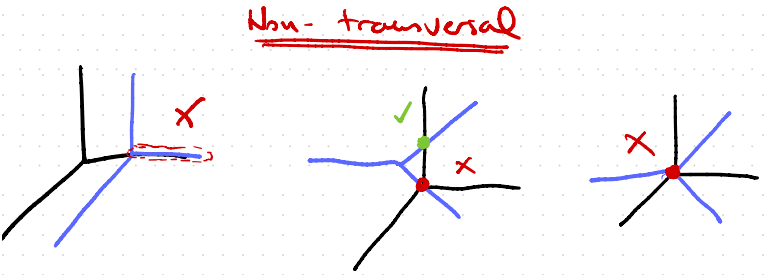
\includegraphics[width=0.5\textwidth]{figs/fig11-2-NonTransversalIntersectionExample.png}
        \caption{Example of Non-Transversal Intersections}
        \label{fig:11.2-NonTransversalIntersectionExample}
    \end{figure}
\end{Ex}

It looks like if the intersection is transversal then the set of intersection is just a point. Otherwise let's be very topological and talk about stable intersections.

\begin{Def}
    For a vector $\vec v\in\bR^2\less\set{0}$, call the \term{vector intersection} of $\Ga_1,\Ga_2$
    $$\Ga_1\cap_{\vec v}\Ga_2=\lim_{t\to 0}\left(\Ga_1\cap(\Ga_2+t\vec c)\right).$$
\end{Def}
\red{FIGURE DRAWING}%PAGE 2/13 TG11
Observe that this definition may be troublesome because of the choice of the vector $\vec v$. What happens if we get another intersection point with another $\vec v$?\par
\red{FIGURE DRAWING}
From this we deduce that intersection points should be weighted by multiplicity of the edges they belong to. We need to build theory in order to consider this idea.\par 
As an aside, let us ask how the curves 
$$C_1=\set{x^a=y^b},\word{and} C_2=\set{x^c=y^d}$$
intersect in $\bC^2$. Observe that we may parametrize $(x,y)=(t^b,t^a)$ and substitute into the other equation to get 
$$t^{bc}(t^{ad-bc}-1)=0$$
which means that at zero we have a point of high multiplicity and $(ad-bc)$ points away from the origin. The interesting question is how does this relate to our problem. And the connection is the valuation. 

\begin{Def}
    Let $p$ be a point of transversal intersection of two tropical curves $\Ga_1,\Ga_2$. Then the multiplicity of the intersection is determined by the primitive directions of the intersection as 
    $$m_p(\Ga_1,\Ga_2)=w_1w_2|\det(p_1,p_2)|=w_1w_2\bonj{\bZ^2\: p_1\bZ+p_2\bZ}.$$
    Where the last quantity is the subgroup index.
\end{Def}

\section{Day 19|20231004}

Our objective last time was to motivate the idea of intersections with certain multiplicity. With out new definition of multiplicity, does this resolve the issue we had? 

\begin{Ex}
\red{FIGURE} 
In the first case we have intersections at $Q_1,Q_2$, where the first intersection has multiplicity
$$m_{Q_1}=\left|\det\twobytwo{0}{1}{1}{-1}\right|$$
and the other point also has multiplicity $1$. But if we move to the non-transversal intersection we get multiplicity $2$. This goes according to the definition. 
\end{Ex}

\begin{Lem}
The amount of intersections of two tropical curves is invariant under generic translation.
\end{Lem}

The proof follows from the balancing conditions and it suffices to analyze cases locally.

\begin{ptcbp}
Consider an edge of a tropical curve and a local intersection. The edge partitions the plane into two half planes $H^+,H^-$. Then the contribution to a $\vec v$ deformed intersection is the same when $\vec v$ points in the direction of $H^+$ or $H^-$.\par 
Suppose $\vec v_1$ and $\vec v_2$ are two vectors pointing in different directions, if we raise the intersection, we get the lower edges intersecting. Their primitive vectors are all in the clockwise direction form $p_e$. So the weight of the $\vec v_1$-deformed intersection is 
           $$\sum_{e'\in E^-}w_ew_{e'}|\det(p_1,p_2)|$$
\end{ptcbp}

\subsection{Tropical Bézout}

From this lemma the result follows immediately!

\begin{Th}
Let $\Ga_1,\Ga_2$ be two tropical curves of degree $d_1,d_2$. Then $|\Ga_1\cap\Ga_2|=d_1d_2$.
\end{Th}

A curve has degree $d$ if its dual to a subdivision of $0,(d,0)$ and $(0,d)$. We know that if we have a tropical curve of degree $d_1$ then we can move one of degree $d_2$ in such a way that just so many edges intersect. Counting down we get the product of the multiplicities.

\section{Day 20|20231009}

Last time we started talking about the idea behind Bézout's theorem. Recall, that a curve with degree $d_i$ is dual to the polygon with vertices $0$, $(0,d_i)$ and $(d_i,0)$. Intersections, as in the ordinary case, are counted with multiplicities.\par 
The quantity $|\Ga_1\cap \Ga_2|$ is invariant under translation, so we can move two curves so that only unbounded ends intersect. Looking at this picture from far away and squinting our eyes what we see is two tripods with degree $d_i$. This means that all the information needed to compute the intersection is independent of the subdivisions of the Newton Polygon.
\begin{Def}
    In $\bP^1\x\bP^1$, coordinates are $([x_0:x_1],[y_0:y_1])$, a \term{bi-degree $(a,b)$ curve} is the zero locus of a bi-homogenous polynomial in the aforementioned variables which is 
    \begin{itemize}
        \item homogenous of degree $a$ is $x_i$,
        \item homogenous of degree $b$ is $y_i$.
    \end{itemize}    
    Tropically, this means that $\Ga$ is dual to a subdivision of a rectangle with sides $a$, $b$.
\end{Def}

\begin{Ex}
    The polynomial $x_0y_0+x_1x_0y_1=0$ is a bidegree $(2,1)$ curve. On the tropical side we have \red{FIGURE} which is a $(1,1)$ curve.
\end{Ex}

The tropical Bézout theorem for $\bP^1\x\bP^1$ says that if we have $\Ga_i$ with bidegree $(a_i,b_i)$, then 
$$|\Ga_1\cap\Ga_2|=a_1b_2+a_2b_1.$$

But what if we wanted to intersect a degree $d$ curve with a bidegree $(a,b)$ curve? We just draw the stick figure and notice that degree of the intersection is $d(a+b)$. We can ask how to generalize it and the answer is precisely Bernstien's theorem.

\begin{Th}
Let $\Ga_i$ be tropical curves of degree $\Dl_i$. Then 
$$|\Ga_1\cap\Ga_2|=\operatorname{MixedArea}(\Dl_1,\Dl_2).$$
\end{Th}

In this case the degree of a tropical curve is the Newton polygon of its equation. In other words a lattice polygon.

\subsection{Minkowski Sum of Polytopes}

Once a long time ago we were told that a degree is a number, but a degree is actually a polygon.
\begin{Def}
    Consider $\Dl_i\subseteq\bR^2$ lattice polygon, then the \term{Minkowski sum} is 
    $$\Dl_1+\Dl_2=\set{(x_1,y_1)+(x_2,y_2)\in\bR^2\:\ (x_i,y_i)\in\Dl_i}.$$
\end{Def}
This definition is \textbf{compatible} with translations! At this moment we can choose how to put two polygons in $\bR^2$ and sum them. 

\begin{Ex}
    The Minkowski sum of a square and a right triangle is a gem-shaped pentagon. The idea is that we decide one of the vertices to be the origin and then make the polygon travel through the perimeter of the other one.
\end{Ex}

\begin{Ej}
The Minkowski sum appears to be commutative, prove it! Which other properties does the Minkowski sum enjoy?
\end{Ej}

\begin{Ex}
\red{FIGURE ABOUT MIXED SUDVISIONS}
\end{Ex}

\begin{Def}
    The \term{mixed area} of $\Dl_1,\Dl_2$ is either of 
    \begin{enumerate}[i)]
        \item $A(\Dl_1+\Dl_2)-A(\Dl_1)-A(\Dl_2)$,
        \item the area of the mixed cells in any mixed subdivision of $\Dl_1+\Dl_2$,
        \item the $\la\mu$ coefficient in $A(\la P+\mu Q)$.
    \end{enumerate}
\end{Def}

\chapter{Toric Varieties}
\section{Day 21|20231011}

IT says that if we have two tropical curves of degree $\Dl_1,\Dl_2$ (polytopes), and we wish to compute the intersections, then this is counted via the mixed area. This correspondence is very tight, satisfying. When taking stuff, we get the mixed cells (parallelograms with sides parallel to our original polygons). Having the polygons in positions means that the curves have been moved and the mixed cells correspond to the intersections.\par 
The weight of the edges is the length of sides of the polygon, in particular the Minkowski sum of two lattice polytopes is itself a lattice polytope.

\subsection{Torus actions}

A space $X$ with a torus action $T\.X$ and an open set isomorphic to the torus on which $T$ acts by multiplication is a toric variety. The geometry of a torus is fairly simple or trivial, which means that \emph{most} of the geometry of $X$ can be recovered from the complement of this dense open set (the one isomorphic to $T$). The fact that we have a torus action allows for a \emph{combinatorialization} of the geometric information.\par 
If we don't know what a torus is, it's a group, and the space is just the space. The action moves the points in a certain way. Geometry is connected to the representation theory of the group.

\begin{Def}
    The \term{algebraic torus} of rank $k$ is $G_m^k$ (think of it as $(\bC^\ast)^k$) \aside[If we have a different field than $\bC$, actually $G$ is a multiplicative group \emph{scheme}]. This object is a group under pointwise multiplication and in general we can view it as the scheme 
    $$\Spec\left(\bC\bonj{x_1,\frac{1}{x_1},\dots,x_k,\frac{1}{x_k}}\right).$$
    If we are more familiar with differential geometry, local coordinates are similar but the coordinate is a generalization. We can imagine elements on the scheme as regular functions from the torus to $\bC$. We will usually denote the torus by $T$.
\end{Def}

Recall a group acts on itself via multiplication and in a similar faction the torus action on a space $X$ will be a map $T\x X\to X$. We can thus relate the characters of $T$ to invertible regular functions on $T$ and if we are choosing coordinates, then they are also related to monomial functions in $x_i$'s.\par 
The characters of $T$ are the group homomorphisms from $T$ to $\bC^\ast$. It is actually the trace of an irreducible representation of $T$, but they are one dimensional and\dots Monomial functions on the $x_i$'s are precisely regular functions vanish. Those places are on the coordinate axis so nowhere near the torus. As a $\bC$-vector space, monomials are a basis of our ring. That is gonna play an important role.\par 
All of these interpretations are groups under multiplication. Given a monomial we can read a vector of exponents: 
$$x^3y^{-5}\mapsto (3,-5)$$
so this is also related to the lattice of exponents of the monomial functions. This gives a multiplicative to additive isomorphism. This lattice is called $M$, it is also called the character lattice and is isomorphic to $\bZ^k\subseteq \bR^k$ which we will also called $M_\bR$. This is actually a \emph{tensor product}. In this sense we can match 
$$(3,-5)\mapsto \vf_{(3,-5)}\: T\to\bC^\ast,\ (t_1,t_2)\mapsto t_1^3t_2^{-5}.$$
We also have a relationship between co-characters (linear functions on characters), one parameter subgroups of $T$ (group homomorphisms $\bC^\ast\to T$, $t\mapsto(t^a,t^b))$. The co-character lattice $N$ is the dual of the character lattice is isomorphic to $\bZ^k\subseteq\bR^k=N_\bR$. There is a natural pairing $M\x N\to\bZ$ which turns out to be the usual dot product. Slightly more satisfying, the natural way to get a pairing is to imagine we have a character $\chi$ and a one parameter subgroup $\ga$ we get a map 
$$\bC^\ast\xrightarrow[]{\chi}T\xrightarrow[]{\ga}\bC^\ast,\ t\mapsto(t^a,t^b)\mapsto t^{aA+bB}$$
so the exponent is precisely $\braket{(a,b)}{(A,B)}$.\par
After talking about so many ingredients, let us talk about one more thing. If we have one parameter subgroups, we can think of them as acting on the torus so we have torus orbits. Let's see some torus orbits we get with different actions. 

\begin{Ex}
    Consider the one parameter subgroup $\ga_{(1,1)}(t)=(t,t)$. Acting on a point $(a,b)$ we get the point $(ta,tb)$. So the orbits are lines through the origin. And notice the in fact, $\ga_{(-1,-1)}(t)=(t^{-1},t^{-1})$, even if we get the same orbits, on the first case we get flow inwards while on the second one we get \emph{outwards} flow.\par 
    We could get $\ga_{(1,0)}(t)=(t,1)$, the orbits are horizontal lines. Finally $\ga_{(1,-1)}(t)=(t,t^{-1})$, then the orbits are hyperbolas. 
\end{Ex}

Now we are gonna say ok, we are gonna allow ourselves to grow the torus a little bit by saying that we want to add limit points of one parameter or allow/decide that some monomial functions are regular and some are not and then add the points. In the case of $\ga_{(1,1)}$ we are going to need to fill in the point of the origin. 
%%%%%%%%%%%% Contents end %%%%%%%%%%%%%%%%

\ifx\nextra\undefined
\printindex
\else\fi
\nocite{*}
\bibliographystyle{plain}
\bibliography{bibiTropiGeo.bib}
\end{document} 

